%%%%%%%%%%%%%%%%%%%%%%%%%%%%%%%%%%%%%%%%%%%%%%%%%%%
%
%  Author: Jacob Vaughn
%
%  Last Updated: 3/8/2024
%
%%%%%%%%%%%%%%%%%%%%%%%%%%%%%%%%%%%%%%%%%%%%%%%%%%%

\documentclass[12pt]{report}

\usepackage{tamuconfig}

%Comment this line if you do not wish to use Times New Roman. The font used will then be the LaTeX default of Computer Modern.
\usepackage{times}
%\usepackage{cmbright}
\usepackage[T1]{fontenc}

%This package allows for the use of graphics in the document.
\usepackage{graphicx}

\DeclareGraphicsExtensions{.png}

\graphicspath{ {../graphics/} }

% For quick document navigation.
\usepackage[hidelinks]{hyperref}

%%%%%%%%%%%%%%%%%%%%%%%%%%%%%%%%%%%%%%%%%%%%%%%%%%%%%%%%%
%Begin student defined packages.
%%%%%%%%%%%%%%%%%%%%%%%%%%%%%%%%%%%%%%%%%%%%%%%%%%%%%%%%%
\usepackage{cite}
\usepackage{gensymb}
\usepackage{caption}
\usepackage{subcaption}
%%%%%%%%%%%%%%%%%%%%%%%%%%%%%%%%%%%%%%%%%%%%%%%%%%%%%%%%%
%End student defined packages.
%%%%%%%%%%%%%%%%%%%%%%%%%%%%%%%%%%%%%%%%%%%%%%%%%%%%%%%%%

% End preamble. Document begins below.

\begin{document}

%The title of your document goes here.
%Spacing may need to be adjusted if your title is long and pushes the copyright off the page.
\renewcommand{\tamumanuscripttitle}{Design, Fabrication, and Characterization of a Low-Disturbance, Actively-Controlled, Mach 5 to 8 Wind Tunnel}

\renewcommand{\tamupapertype}{Dissertation Proposal}

\renewcommand{\tamufullname}{Jacob B. Vaughn}

%The degree title goes here.
\renewcommand{\tamudegree}{Doctor of Philosophy}
\renewcommand{\tamuchairone}{Edward White}

%Committee members
\renewcommand{\tamumemberone}{Rodney Bowersox}
\newcommand{\tamumembertwo}{Nathan Tichenor}
\newcommand{\tamumemberthree}{Je Han}
\renewcommand{\tamudepthead}{Ivett Leyva}

\renewcommand{\tamugradmonth}{March}
\renewcommand{\tamugradyear}{2024}
%Your department name goes here.
\renewcommand{\tamudepartment}{Aerospace Engineering}

%%%%%%%%%%%%%%%%%%%%%%%%%%%%%%%%%%%%%%%%%%%%%%%%%%%
%
%  Author: Jacob Vaughn 
%  
%  Last Updated: 1/10/2024
%
%%%%%%%%%%%%%%%%%%%%%%%%%%%%%%%%%%%%%%%%%%%%%%%%%%%

%%%%%%%%%%%%%%%%%%%%%%%%%%%%%% 
%% TITLE PAGE
%% The values get updated automatically.  Please do not make changes to this file other than adding/deleting committee members where necessary.
%%%%%%%%%%%%%%%%%%%%%%%%%%%%%%

\providecommand{\tabularnewline}{\\}



\begin{titlepage}
\begin{center}
\begin{doublespace}

\MakeUppercase{  \tamumanuscripttitle}
\end{doublespace}
\vspace{4em}

A \tamupapertype

by

\MakeUppercase{\tamufullname}

\vspace{4em}

\begin{singlespace}

Submitted to the Graduate and Professional School of \\
Texas A\&M University \\

in partial fulfillment of the requirements for the degree of \\
\end{singlespace}

\MakeUppercase{\tamudegree}
\par\end{center}
\vspace{2em}
\begin{doublespace}

\end{doublespace}
\begin{tabular}{ll}
 & \tabularnewline
& \cr
% If you have Co-Chairs comment out the 'Chair of Committee' line below and uncomment the 'Co-Chairs of Committee' line.
Chair of Committee, & \tamuchairone\tabularnewline
%Co-Chairs of Committee, & \tamuchairone\tabularnewline & \tamuchairtwo\tabularnewline
Committee Members, & \tamumemberone\tabularnewline
 & \tamumembertwo\tabularnewline
 & \tamumemberthree\tabularnewline
Head of Department, & \tamudepthead\tabularnewline

\end{tabular}

\vspace{3em}

\begin{center}
\tamugradmonth \hspace{2pt} \tamugradyear

\vspace{3em}

Major Subject: \tamudepartment \par
\vspace{3em}
Copyright \tamugradyear \hspace{.5em}\tamufullname 
\par\end{center}
\end{titlepage}
\pagebreak{}




 

% %%%%%%%%%%%%%%%%%%%%%%%%%%%%%%%%%%%%%%%%%%%%%%%%%%%
%
%  Author: Jacob Vaughn
%  
%  Last Updated: 1/10/2024
%
%%%%%%%%%%%%%%%%%%%%%%%%%%%%%%%%%%%%%%%%%%%%%%%%%%%
%%%%%%%%%%%%%%%%%%%%%%%%%%%%%%%%%%%%%%%%%%%%%%%%%%%%%%%%%%%%%%%%%%%%%
%%                           ABSTRACT 
%%%%%%%%%%%%%%%%%%%%%%%%%%%%%%%%%%%%%%%%%%%%%%%%%%%%%%%%%%%%%%%%%%%%%

\chapter*{ABSTRACT}
\addcontentsline{toc}{chapter}{ABSTRACT} % Needs to be set to part, so the TOC doesn't add 'CHAPTER ' prefix in the TOC.

\pagestyle{plain} % No headers, just page numbers
\pagenumbering{roman} % Roman numerals
\setcounter{page}{2}

\indent This is the first numbered page, lower case Roman numeral (ii). Page numbers are outside the prescribed margins, at the bottom of the page and centered; everything else is inside the margins.No bold on this page except the heading ABSTRACT if all major headings are bold. \emph{This \LaTeX ~ template applies to this exception}).

Text begins two double spaces below the major heading. The Abstract should be no more than 350 words. Vertical spacing is double spaced. (\emph{This \LaTeX ~ template applies double space for this ABSTRACT.}) The margin settings and text alignment should be consistent throughout the document. There should be no numbered references or formal citations in ABSTRACT.

The content of this ABSTRACT provides a complete, short snapshot of the research, addressing the purpose, methods, results, and conclusions of the document. As a result, it should stand alone without any formal citations or references to chapters/sections of the work. To accommodate with a variety of online database, images, complex equations, or Greek letters/symbols should also be avoided.This should be no longer than 350 words.

The next pages are Dedication, Acknowledgments, Contributors and Funding Sources, and Nomenclature. Contributors and Funding Sources is required, the rest are optional.


 

\pagebreak{}

% %%%%%%%%%%%%%%%%%%%%%%%%%%%%%%%%%%%%%%%%%%%%%%%%%%%
%
%  New template code for TAMU Theses and Dissertations starting Spring 2021.  
%
%
%  Author: Thesis Office
%  
%  Last Updated: 1/13/2021
%
%%%%%%%%%%%%%%%%%%%%%%%%%%%%%%%%%%%%%%%%%%%%%%%%%%%

%%%%%%%%%%%%%%%%%%%%%%%%%%%%%%%%%%%%%%%%%%%%%%%%%%%%%%%%%%%%%%%%%%%%%%
%%                           DEDICATION
%%%%%%%%%%%%%%%%%%%%%%%%%%%%%%%%%%%%%%%%%%%%%%%%%%%%%%%%%%%%%%%%%%%%%
\chapter*{DEDICATION}
\addcontentsline{toc}{chapter}{DEDICATION}  % Needs to be set to part, so the TOC doesnt add 'CHAPTER ' prefix in the TOC.



\begin{center}
\vspace*{\fill}
To my mother, father, grandfather, and grandmother. I'm filling in more space so that this extends to the next line. 
\vspace*{\fill}
\end{center}

\pagebreak{}

% %%%%%%%%%%%%%%%%%%%%%%%%%%%%%%%%%%%%%%%%%%%%%%%%%%%
%
%  New template code for TAMU Theses and Dissertations starting Fall 2016.  
%
%
%  Author: Thesis Office
%  
%  Last Updated: 1/13/2021
%
%%%%%%%%%%%%%%%%%%%%%%%%%%%%%%%%%%%%%%%%%%%%%%%%%%%


%%%%%%%%%%%%%%%%%%%%%%%%%%%%%%%%%%%%%%%%%%%%%%%%%%%%%%%%%%%%%%%%%%%%%%
%%                           ACKNOWLEDGMENTS
%%%%%%%%%%%%%%%%%%%%%%%%%%%%%%%%%%%%%%%%%%%%%%%%%%%%%%%%%%%%%%%%%%%%%
\chapter*{ACKNOWLEDGMENTS}
\addcontentsline{toc}{chapter}{ACKNOWLEDGMENTS}  % Needs to be set to part, so the TOC doesnt add 'CHAPTER ' prefix in the TOC.


\indent This section is also optional, and limited to four pages. It must follow the Dedication Page (or Abstract, if there's no Dedication). If listing preliminary pages in Table of Contents, include Acknowledgments. This heading (\MakeUppercase{Acknowledgments}) is bold if major headings are bold. It should be in same type size and style as text. As does the vertical spacing, paragraph style, and margins. 

I would like to thank the Texas A\&M University Graduate and Professional School to allow me to construct this \LaTeX\ thesis template.  % use A\&M instead of A$\&$M, not use $A\&M$ as well, the last one won't be bold.



\pagebreak{}
% %%%%%%%%%%%%%%%%%%%%%%%%%%%%%%%%%%%%%%%%%%%%%%%%%%%
%
%  Author: Jacob Vaughn
%  
%  Last Updated: 1/13/2024
%
%%%%%%%%%%%%%%%%%%%%%%%%%%%%%%%%%%%%%%%%%%%%%%%%%%%

%%%%%%%%%%%%%%%%%%%%%%%%%%%%%%%%%%%%%%%%%%%%%%%%%%%%%%%%%%%%%%%%%%%%%%
%%             CONTRIBUTORS AND FUNDING SOURCES
%%%%%%%%%%%%%%%%%%%%%%%%%%%%%%%%%%%%%%%%%%%%%%%%%%%%%%%%%%%%%%%%%%%%%
\chapter*{CONTRIBUTORS AND FUNDING SOURCES}
\addcontentsline{toc}{chapter}{CONTRIBUTORS AND FUNDING SOURCES}  % Needs to be set to part, so the TOC doesn't add 'CHAPTER ' prefix in the TOC.

\subsection*{Contributors}
This work was supported by a thesis (or) dissertation committee consisting of Professor John Doe [advisor --– also note if co-advisor] and John Doe of the Department of [Home Department] and Professor(s) XXXX of the Department of [Other Department].

The data analyzed for Chapter IV was provided by Professor Thompson. The analyses depicted in Chapter X were conducted in part by Daniel James of the Department of Statistics and were published in (2004) in an article listed in the Journal of Things.

All other work conducted for the thesis (or) dissertation was completed by the student independently.
\subsection*{Funding Sources}
Graduate study was supported by a fellowship from Texas A\&M University and a dissertation research fellowship from That Foundation. OR No other outside source of funding was provided. One or the other must be stated.


\pagebreak{}

%%%%%%%%%%%%%%%%%%%%%%%%%%%%%%%%%%%%%%%%%%%%%%%%%%%
%
%  New template code for TAMU Theses and Dissertations starting Spring 2021.  
%
%
%  Author: Thesis Office
% 
%  Last Updated: 1/13/2021
%
%%%%%%%%%%%%%%%%%%%%%%%%%%%%%%%%%%%%%%%%%%%%%%%%%%%

%%%%%%%%%%%%%%%%%%%%%%%%%%%%%%%%%%%%%%%%%%%%%%%%%%%%%%%%%%%%%%%%%%%%%%
%%                           NOMENCLATURE
%%%%%%%%%%%%%%%%%%%%%%%%%%%%%%%%%%%%%%%%%%%%%%%%%%%%%%%%%%%%%%%%%%%%%

\chapter*{NOMENCLATURE}
\addcontentsline{toc}{chapter}{NOMENCLATURE}  % Needs to be set to part, so the TOC doesnt add 'CHAPTER ' prefix in the TOC.

%A note about aligning: These entries will align
%themselves according to the ampersand (&).
%No extra spaces are needed, as seen in some of
%the entries below.

%Example of the longtable environment.
\hspace*{-1.25in}
\vspace{12pt}
\begin{spacing}{1.0}
	\begin{longtable}[htbp]{@{}p{0.35\textwidth} p{0.62\textwidth}@{}}
	   % \begin{tabular}{@{}p{0.33\textwidth} p{0.62\textwidth}@{}}
		OGAPS	&	Office of Graduate and Professional Studies at Texas A\&M University\\	[2ex]
		B/CS		&	Bryan and College Station\\	[2ex] %[2ex] provides double space between each row
		TAMU			&	Texas A\&M University\\	[2ex]
		SDCC & San Diego Comic-Con\\ [2ex]
		EVIL & Every Villain is Lemons\\ [2ex]
		EPCC & Educator Preparation and Certification Center at Texas A\&M University - San Antonio\\ [2ex]
		FFT & Fast Fourier Transform\\ [2ex]
		ARIMA & Autoregressive Integrated Moving Average\\ [2ex]
		SSD & Solid State Drive\\ [2ex]
		HDD & Hard Disk Drive\\ [2ex]
		O\&M & Eller Oceanography and Meteorology Building\\ [2ex]
		DOS & Disk Operating System\\ [2ex]
		HDMI & High Definition Multimedia Interface\\ [2ex]
		$L^1$ & Space of absolutely Lebesgue integrable functions; i.e., $\int |f| < \infty$\\ [2ex]
		$L^2$ & Space of square-Lebesgue-integrable functions, i.e., $\int |f|^2 < \infty$\\ [2ex]
		$PC(S)$ & Space of piecewise-continuous functions on $S$\\ [2ex]
		GNU & GNU is Not Unix\\ [2ex]
		GUI & Graphical User Interface\\ [2ex]
		PID & Principal Integral Domain\\ [2ex]
		MIP & Mixed Integer Program\\ [2ex]
		LP & Linear Program\\ [2ex]
		%XXXXXXXX		&	This is an optional page. Random word to test how long the sentence can be? This is just for test purpose. The current setting aims to align left/right margin same as all other pages.\\	[2ex]
	   % \end{tabular}%
	\end{longtable}
\end{spacing}

\pagebreak{}

%%%%%%%%%%%%%%%%%%%%%%%%%%%%%%%%%%%%%%%%%%%%%%%%%%%
%
%  Author: Jacob Vaughn
% 
%  Last Updated: 1/13/2024
%
%%%%%%%%%%%%%%%%%%%%%%%%%%%%%%%%%%%%%%%%%%%%%%%%%%%
%%%%%%%%%%%%%%%%%%%%%%%%%%%%%%%%%%%%%%%%%%%%%%%%%%%%%%%%%%%%%%%%%%%%%%
%%       TABLE OF CONTENTS
%%%%%%%%%%%%%%%%%%%%%%%%%%%%%%%%%%%%%%%%%%%%%%%%%%%%%%%%%%%%%%%%%%%%%

\phantomsection
\addcontentsline{toc}{chapter}{TABLE OF CONTENTS}  

\begin{singlespace}
\renewcommand\contentsname{\normalfont} {\centerline{TABLE OF CONTENTS}}

\setcounter{tocdepth}{4} % This puts \subsubsection[]{×} in your List of Tables.  The default is 3.


%%%%%%%%%%%%%  Adds Page above the page number in TOC
\setlength{\cftaftertoctitleskip}{1em}
\renewcommand{\cftaftertoctitle}{%
\hfill{\normalfont {Page}\par}}


\tableofcontents

%\addtocontents{toc}{\protect\afterpage{~\hfill\normalfont{Page}\par\medskip}}
\end{singlespace}

\pagebreak{}

%%%%%%%%%%%%%%%%%%%%%%%%%%%%%%%%%%%%%%%%%%%%%%%%%%%%%%%%%%%%%%%%%%%%%%
%%                           LIST OF FIGURES
%%%%%%%%%%%%%%%%%%%%%%%%%%%%%%%%%%%%%%%%%%%%%%%%%%%%%%%%%%%%%%%%%%%%%

\phantomsection
\addcontentsline{toc}{chapter}{LIST OF FIGURES}  

\renewcommand{\cftloftitlefont}{\center\normalfont\MakeUppercase}

\setlength{\cftbeforeloftitleskip}{-12pt} %% Positions the LOF title vertically to match the chapter titles
\renewcommand{\cftafterloftitleskip}{12pt}


\renewcommand{\cftafterloftitle}{%
\\[4em]\mbox{}\hspace{2pt}FIGURE\hfill{\normalfont Page}\vskip\baselineskip}

\begingroup


\begin{center}
\begin{singlespace}
%% These values make the lof table entries appear double spaced between.
\setlength{\cftbeforechapskip}{0.4cm}
\setlength{\cftbeforesecskip}{0.30cm}
\setlength{\cftbeforesubsecskip}{0.30cm}
\setlength{\cftbeforefigskip}{0.4cm}
\setlength{\cftbeforetabskip}{0.4cm}

% Provided by Andy Philips.
% needed to make chapter gaps look no different than sections:
% \addtocontents{lof}{\protect\renewcommand*\protect\addvspace[1]{}}

% Philips' document had 30 figures. Is there a maximum number of figures
% that changes the spacing to non-uniform, i.e., not double-spaced
% between all entries?

\listoffigures

\end{singlespace}
\end{center}

\pagebreak{}


%%%%%%%%%%%%%%%%%%%%%%%%%%%%%%%%%%%%%%%%%%%%%%%%%%%%%%%%%%%%%%%%%%%%%%
%%                           LIST OF TABLES
%%%%%%%%%%%%%%%%%%%%%%%%%%%%%%%%%%%%%%%%%%%%%%%%%%%%%%%%%%%%%%%%%%%%%%
%
\phantomsection
\addcontentsline{toc}{chapter}{LIST OF TABLES}  

\renewcommand{\cftlottitlefont}{\center\normalfont\MakeUppercase}

\setlength{\cftbeforelottitleskip}{-12pt} %% Positions the LOT title vertically to match the chapter titles

%Note that the similar parameter in the LOF is 12pt; this
%is intentional to make the spacing between the headers
%and the first entry look consistent.
\renewcommand{\cftafterlottitleskip}{1pt}


\renewcommand{\cftafterlottitle}{%
\\[4em]\mbox{}\hspace{2pt}TABLE\hfill{\normalfont Page}\vskip\baselineskip}

\begin{center}
\begin{singlespace}

%% These values make the lot table entries appear double spaced between.
\setlength{\cftbeforechapskip}{0.4cm}
\setlength{\cftbeforesecskip}{0.30cm}
\setlength{\cftbeforesubsecskip}{0.30cm}
\setlength{\cftbeforefigskip}{0.4cm}
\setlength{\cftbeforetabskip}{0.4cm}

\listoftables 

\end{singlespace}
\end{center}
\endgroup
\pagebreak{}  % Need this for the page numbering to be correct. 
  

%%%%%%%%%%%%%%%%%%%%%%%%%%%%%%%%%%%%%%%%%%%%%%%%%%%
%
%  Author: Jacob Vaughn
%  
%  Last Updated: 3/8/2024
%
%%%%%%%%%%%%%%%%%%%%%%%%%%%%%%%%%%%%%%%%%%%%%%%%%%%

%%%%%%%%%%%%%%%%%%%%%%%%%%%%%%%%%%%%%%%%%%%%%%%%%%%%%%%%%%%%%%%%%%%%%%
%%                         INTRODUCTION
%%%%%%%%%%%%%%%%%%%%%%%%%%%%%%%%%%%%%%%%%%%%%%%%%%%%%%%%%%%%%%%%%%%%%


\pagestyle{plain} % No headers, just page numbers
\pagenumbering{arabic} % Arabic numerals
\setcounter{page}{1}


\chapter{INTRODUCTION \& LITERATURE REVIEW}

\section{Introduction}

In recent decades, the continual improvement in hypersonic aerodynamics has emphasized the need for advancements in wind tunnel ground testing capabilities \cite{leyva}. Conventional hypersonic wind tunnels rely on distinct fixed nozzle contours to accelerate the flow to the desired Mach number. This approach fixes the Mach number so it only provides a particular flow regime for experiments. Recognizing this, there is a clear need for a continuously variable Mach-number nozzle designed to overcome the limitations of conventional wind tunnels and enable more advanced dynamic hypersonic research.

The objective of this work is to introduce a continuously variable and actively controllable Mach-number nozzle. By dynamically adjusting the throat height and thereby the Mach number throughout the wind tunnel runs, the variable conditions experienced by hypersonic vehicles during different flight trajectories can be effectively modeled. This capability would enable the advancement of ground testing for a more comprehensive understanding of dynamic hypersonic flight and associated phenomena. Furthermore, the active control capability will increase experimental efficiency by allowing measurements at different Mach numbers within a single run and introduce the ability to fine tune the Mach number for improved data quality. However, this variable Mach number capability does introduce the challenge of maintaining desired Reynolds numbers, so feedback control will also be explored for the Reynolds number to counteract this and improve the overall experimental control.

The Actively Controlled Expansion (ACE) wind tunnel at Texas A\&M University has served as a workhorse in hypersonic research since 2010 \cite{ace09,ace10-calibrate,tichenor-dis,aceturb,mai-dis,neel-dis,leidy-dis}, and is due for improvements to meet the growing demand of hypersonics research. Although the facility was initially designed to facilitate the continuous variation of Mach number, the mechanical implementation ultimately proved to be cumbersome to adjust. Consequently, the nozzle has remained fixed at Mach 6 for the majority of the tunnel's operation, \textcolor{red}{falling short of fully realizing its designated variable Mach capability}. Additionally, despite the geometry being fixed, the Mach number actually varies throughout a run by up to 5\%. \textcolor{red}{Considering this, it is apparent that an update to the ACE nozzle is necessary to remedy these shortcomings.}

\section{Research Objectives}

The objectives of this research aim to lay the foundation for continuously variable and actively controlled Mach number capabilities at the National Aerothermochemistry and Hypersonics Laboratory (NAHL). Doing so will expand the current capabilities within the lab for more advanced hypersonic aerodynamics experiments. This will help maintain the NAHL as a cutting-edge national research facility. The existing ACE facility will be upgraded to achieve true active control and to potentially produce low-disturbance flow for higher Reynolds numbers. Its successor, ACE2.0, that is the subject of this work, will employ a feedback-control system with servo motors, linear actuators, and various instrumentation to enable the accurate and continuous variation of Mach number by changing the throat height. Additionally, active feedback-control of the Reynolds number will be developed and potentially implemented. 

Once fabricated and calibrated, the ACE2.0 facility will provide:

\begin{enumerate}[listparindent=\parindent]
    \item Improved experimental control and efficiency
            
        An active throat height control system will be implemented to enable active feedback-controlled Mach number variation and selection for Mach trajectories and accurate set points. The feedback aspect will attempt to control the Mach number to within 0.5\% of the set value. An active control scheme will also be developed to enable feedback-controlled Reynolds number variation and selection that responds to changes in Mach number and stagnation temperature for accurate sweeps and set points. This will allow both constant or varying Reynolds number during a Mach trajectory. The Reynolds number controller will be fully designed but may not be implemented due to constraints.

        The control of both of these parameters will yield improved experimental efficiency with a new capability to explore multiple flow configurations within a single run. Besides enhancing efficiency, the Mach number and Reynolds number control will enable more robust uncertainty quantification and more dynamic experiments that were not possible before. Both of these capabilities are demonstrated in the next objectives.

    \item Characterization of freestream flow uniformity and disturbance levels throughout the nozzle and uncertainty quantification of flow parameters

        A flow survey of the nozzle exit plane and centerline will be conducted to measure the freestream flow uniformity and disturbance levels throughout the nozzle and characterize its performance. This will validate the design and manufacturing of the nozzle and settling chamber and provide a basis for the quality of data gathered in future experiments. A rigorous uncertainty analysis will be performed to quantify the systematic and random uncertainty of the measured flow parameters $P$, $P_0$, and $T_0$ and the resulting values of Mach number, $M$, and unit Reynolds number, $Re'$. This will establish the baseline uncertainty for the freestream flow parameters and enable improved data quality for future experiments. In order to fully characterize the tunnel behavior while actively controlled, an investigation of the potential existence of hysteresis phenomena will be performed. If discovered, any hysteresis will be characterized to fully understand the dynamics of the freestream flow as each parameter is varied.

    \item Demonstration of Mach trajectory operation and potential hysteresis in a proof of concept experiment

        The capabilities of ACE2.0 will be demonstrated in an experiment that will showcase shock wave interactions between two wedges during a Mach trajectory. This experiment will explore a well-known hysteresis in the transition from a regular reflection to a mach reflection and the ability to produce the phenomenon in this facility. 

\end{enumerate}

These objectives will effectively validate and demonstrate the capabilities and merit of the new ACE2.0 facility. In addition, the standard operating procedures for ACE2.0 will be updated to reflect the best practices deduced throughout the completion of these objectives. The resulting control procedures and interface will be straightforward and well documented so that future users can easily learn to effectively operate the facility. The documentation will not only enhance the accessibility of ACE2.0 for subsequent research endeavors but also contribute to the broader scientific community by providing a robust framework for effective wind tunnel control and dynamic hypersonic vehicle aerodynamics exploration.

\section{Literature Review}

The literature review for this dissertation includes four parts related to hypersonic variable Mach-number wind tunnels and according to the above objectives: (1) variable mach number nozzle design, (2) parameter control, (3) flow quality characterization and uncertainty quantification, and (4) hysteresis in hypersonic flows. This review will discuss articles that establish the most current knowledge base and techniques in the relevant areas of hypersonic wind tunnel research.

\subsection{Variable Mach-Number Wind Tunnels}
Variable Mach number nozzles have been explored in many configurations since the 1950s such as interchangeable fixed-block, plug-type, asymmetric sliding blocks, tilting plate, fully flexible, and hinged/flexure \cite{agard-ag-3}. Each of these designs have varying degrees of flow quality, cost effectiveness, and experimental efficiency that must be considered. Only the fully flexible and flexure designs maximize experimental efficiency without sacrificing flow quality. Of these two, the flexure design minimizes costs by reducing mechanical complexity and supporting structure. Therefore, the flexure design is the optimal choice considering these criteria.

The flexure type nozzle was first proposed in 1955 by Rosen \cite{rosen} and improved upon separately by Erdmann in 1971\cite{erdmann} and Rom and Etsion in 1972 \cite{erdmann,rom} in order to minimize the mechanical complexity. This simple nozzle design operated by a single jack greatly reduces manufacturing and controls costs and allows for greater flexibility in active control to quickly and continuously vary the Mach number to model dynamic supersonic vehicle flight.

In the last decade, many variable mach number supersonic wind tunnels have been manufactured due to increased demand of hypersonic flight research. The majority of these are fully flexible or flexure nozzle designs with varying implementations of actuation and control \cite{ilic-1,shahrbabaki-1,durand,laguarda,chen,guo,lv,qi,steeves}. All of these facilities were developed to study vehicle flight trajectory and the hysteresis phenomenon therein.

\textcolor{red}{Duplicate at start of chapter 2?} The ACE tunnel, the facility of interest for this work, has been in operation since 2010 \cite{ace09,ace10-calibrate,tichenor-dis}. The nozzle is a flexure type that produces Mach 5 to 8 flow in a 9 inch by 14 inch test section. The flexure design is effective in achieving the change in throat height, but it cannot be done continuously and actively during a run. This is the primary issue to be addressed in this work.

\begin{figure}[ht!]
    \centering
    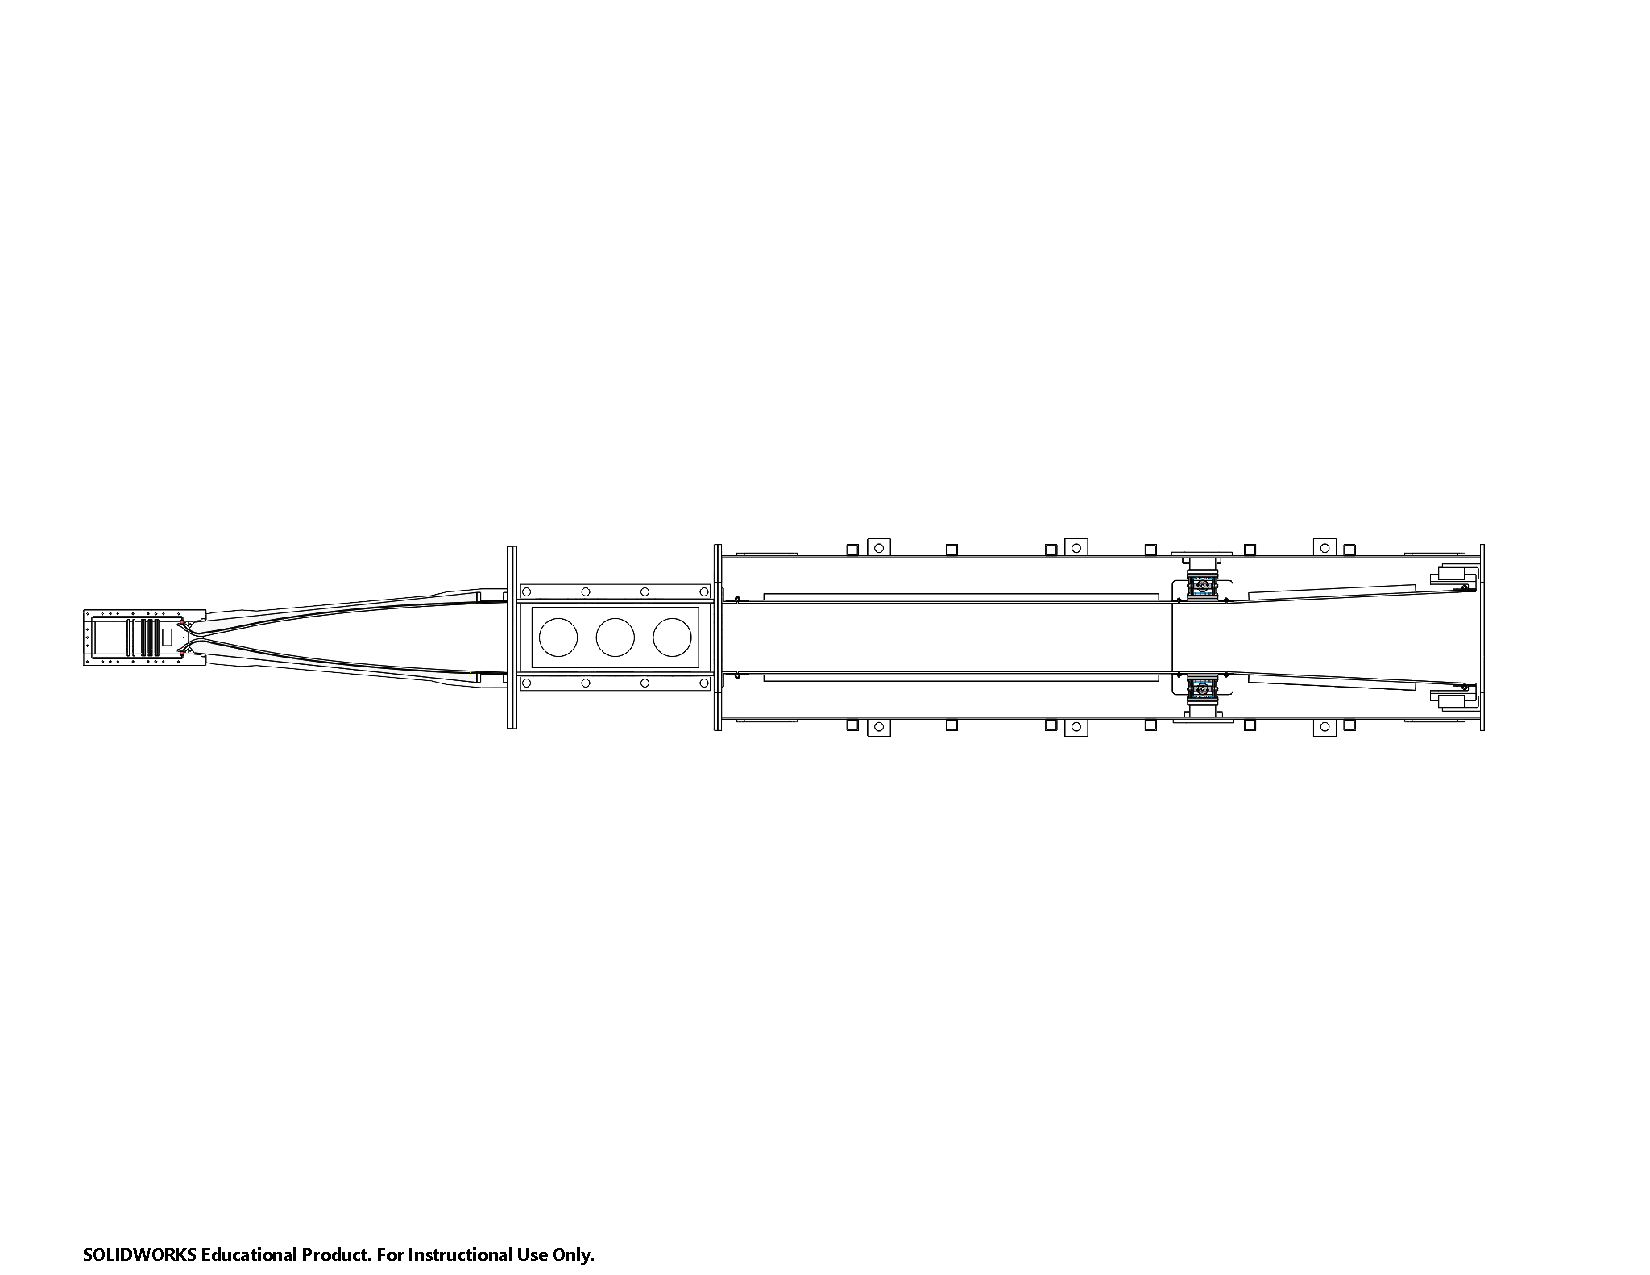
\includegraphics[trim={40 250 60 250},clip,width=6in]{ace-full-tunnel.pdf}
    \caption{ACE tunnel schematic}
    \label{fig:ace-full-tunnel}
\end{figure}

\subsection{Parameter Control}
A variable Mach number facility requires effective control schemes for the controllable parameters $A^*$, $P_0$, $T_0$, and the resulting Mach number, $M$, and unit Reynolds number, $Re'$, in order to vary each parameter independently and accurately. This control problem, acknowledged as early as the 1980s, prompted the development of diverse solutions implementing the various areas of control theory such as optimal control \cite{kraft,hwang}, state feedback control, mathematical model prediction control, preprogrammed controllers \cite{matsumoto}, and PID control \cite{fung,ilic-2,silva}.

In recent years, researchers at numerous variable Mach number facilities have embraced advanced intelligent control methods. Techniques such as fuzzy logic, genetic algorithms, neural networks, adaptive control or gain scheduling, and their combinations have been applied \cite{nott,shahrbabaki-1}. The methods that will be explored in this research are those of Hwang et al. \cite{hwang}, Matsumoto et al. \cite{matsumoto}, Ili\'c et al. \cite{ilic-2}, and Shahrbabaki et al. \cite{shahrbabaki-1} as they each introduce the different advantages and challenges of each control technique. 

Hwang et al. \cite{hwang} developed a robust LQG/LTR (Linear Quadratic Gaussian with Loop Transfer Recovery) controller enhanced by an anti-integrator windup and a modified Smith predictor to overcome unavoidable modeling errors, uncertainties, and time-delay effects. This controller demonstrated a faster stabilization and exhibited fewer oscillations in comparison to its PID counterpart. Given its superior performance, it presents an appealing prospect for implementation in ACE2.0, and a detailed exploration of this controller will be undertaken in a subsequent chapter.

Matsumoto et al. \cite{matsumoto} took a simplified approach by replacing an existing real-time PID controller with a preprogrammed controller to avoid input time delays. This was advantageous for the facility used in that work because the run time was not much longer than the time delay for the PID controller to stabilize. This is the most straightforward approach to obtain specific constant or dynamic trajectories of multiple input parameters but it has limitations. The controller must have a new program for each individual desired parameter set condition or path, and each program must be iterated to minimize errors. Considering these limitations, a preprogrammed controller will be a backup option that will only be explored if necessary. Considering the longer run times of ACE2.0, a PID controller can be implemented with ample time to stabilize.

Ili\'c et al. \cite{ilic-2} implemented a cascade nonlinear feedforward-feedback PID controller as a combined system to enhance a standard single-loop PID. The system's set point reference tracking is improved by the feedforward-feedback architecture, and the disturbance rejection is improved by the cascade architecture. With these two architectures combined in one multi-loop controller, large transient overshoots are eliminated, set point settling times are decreased, and the overall accuracy of the controlled parameters is maximized. Once again, the improved performance of this controller makes it another appealing prospect for ACE2.0, which will be discussed later.

Shahrbabaki et al. \cite{shahrbabaki-1} utilized an artificial neural network and fuzzy logic to enhance a conventional PD controller to handle the complex nonlinearity of the variable mach number wind tunnel flow parameters. The advantages of fuzzy logic include its simplicity and adaptability of introducing new control rules to handle imprecise data, uncertainty, and unmodeled dynamics. The combined advantage that Shahrbabaki et al. explores pertains to the utilization of the neural network to develop the membership functions for the fuzzy logic controller. They designed and trained a feed-forward multilayer perceptron neural network according to the database from the mathematical model of the wind tunnel behavior in order to develop the optimal membership functions. This method will only be explored further for ACE2.0 if the methods of Hwang et al. or Ili\'c et al. do not yield sufficient performance.

\subsection{Flow Quality Characterization and Uncertainty Quantification}
The primary references regarding flow quality characterization will be the recent AIAA articles by Chou et al. \cite{chou} and Duan et al. \cite{duan} on hypersonic wind tunnel freestream disturbance measurements. These provide the latest measurement processes and procedures and reference over 50 publications on relevant topics from recent decades. In addition to these two references, a decade of NAHL experience and best practices will guide the characterization of ACE2.0 upon its fabrication and initial shakedown. Key NAHL ACE references on the freestream characterization of ACE are the AIAA paper by Semper et al. \cite{aceturb} and multiple dissertations by Mai \cite{mai-dis}, Neel \cite{neel-dis}, and Leidy \cite{leidy-dis}. Additionally, Leidy performed an uncertainty analysis in the existing ACE tunnel that will provide a rough baseline reference for the uncertainty quantification for ACE2.0.

The primary references for the uncertainty quantification in this research will be the NASA report by Stephens et al. \cite{stephens-hubbard}, the forthcoming AIAA Guide on Uncertainty Quantification \cite{uq-aiaa}, and the dissertation by Curriston \cite{curriston-dis}. The methodology in this NASA report combines the techniques of the prevalent literature on the subject from the last few decades to quantify the uncertainty of the flow parameters in a supersonic wind tunnel. Curriston's work provides a secondary reference as he thoroughly demonstrates this methodology and that of the forthcoming AIAA guide as a case study in a low speed wind tunnel. The approach described in these references includes a sophisticated treatment of systematic uncertainty using a Mont Carlo method combined with direct comparison of replicate data to characterize random error. Curriston \cite{curriston-dis} also extensively treats pre-test and real-time uncertainly quantification to enhance test campaign quality control and decision support.

\subsection{Hysteresis in Hypersonic Flows}
A review of the literature on hypersonic flow hysteresis yielded many publications discussing shock interactions and inlet start/unstart processes. The inlet start/unstart literature will not be referenced directly in this work but will be valuable for future research in ACE2.0. Focusing on the shock interactions, Hornung et al. \cite{hornung-1} first predicted hysteresis in the transition from regular reflection to Mach reflection, but they were unable to experimentally produce the hysteresis effect \cite{hornung-2}. Recent literature reveals numerical investigations easily reproduce shock interaction hysteresis \cite{chpoun-1,ivanov-3}, while experimental investigations prove more difficult due to the freestream noise in conventional facilities \cite{ben-dor-1,laguarda}. The two processes that produce hysteresis in the shock interactions are wedge-angle variation and Mach-number variation \cite{ben-dor-2}. Since it is significantly more complex to vary the Mach number, most experimental results are found by the wedge-angle-variation-induced hysteresis in open-jet, low-noise wind tunnels \cite{chpoun-2,li,ivanov-4,mouton,setoguchi,chanetz}. Some research groups with variable Mach number tunnels have attempted to reproduce shock interaction hysteresis experimentally by varying the Mach number, but they have all been unsuccessful due to the presence of high freestream disturbance levels \cite{durand,tao}. Methodologies from the numerical and experimental literature on Mach-number-variation-induced hysteresis will be studied in order to attempt to reproduce shock interaction hysteresis in ACE2.0.


%%%%%%%%%%%%%%%%%%%%%%%%%%%%%%%%%%%%%%%%%%%%%%%%%%%
%
%  Author: Jacob Vaughn
%  
%  Last Updated: 3/8/2024
%
%%%%%%%%%%%%%%%%%%%%%%%%%%%%%%%%%%%%%%%%%%%%%%%%%%%

%%%%%%%%%%%%%%%%%%%%%%%%%%%%%%%%%%%%%%%%%%%%%%%%%%%%%%%%%%%%%%%%%%%%%%%
%%%               DESIGN AND FABRICATION OF ACE2.0
%%%%%%%%%%%%%%%%%%%%%%%%%%%%%%%%%%%%%%%%%%%%%%%%%%%%%%%%%%%%%%%%%%%%%%


\chapter{DESIGN AND FABRICATION OF ACE2.0}

\section{Background and Motivation}

\textcolor{red}{Should this paragraph be here or in lit review or both?} The existing ACE tunnel was designed and manufactured between 2009 and 2010 and began operating in 2010 \cite{ace09,ace10-calibrate,tichenor-dis}. The nozzle is 40 inches long from the throat to the test section entrance. The test section is 14 inches wide and 9 inches tall. The last 4 inches of the nozzle is a thin flexure portion that allows the throat height to be varied from approximately 0.04 to 0.36 inches, which enables the test-section Mach number to be varied from Mach 5 to 8.

\begin{figure}[ht!]
    \centering
    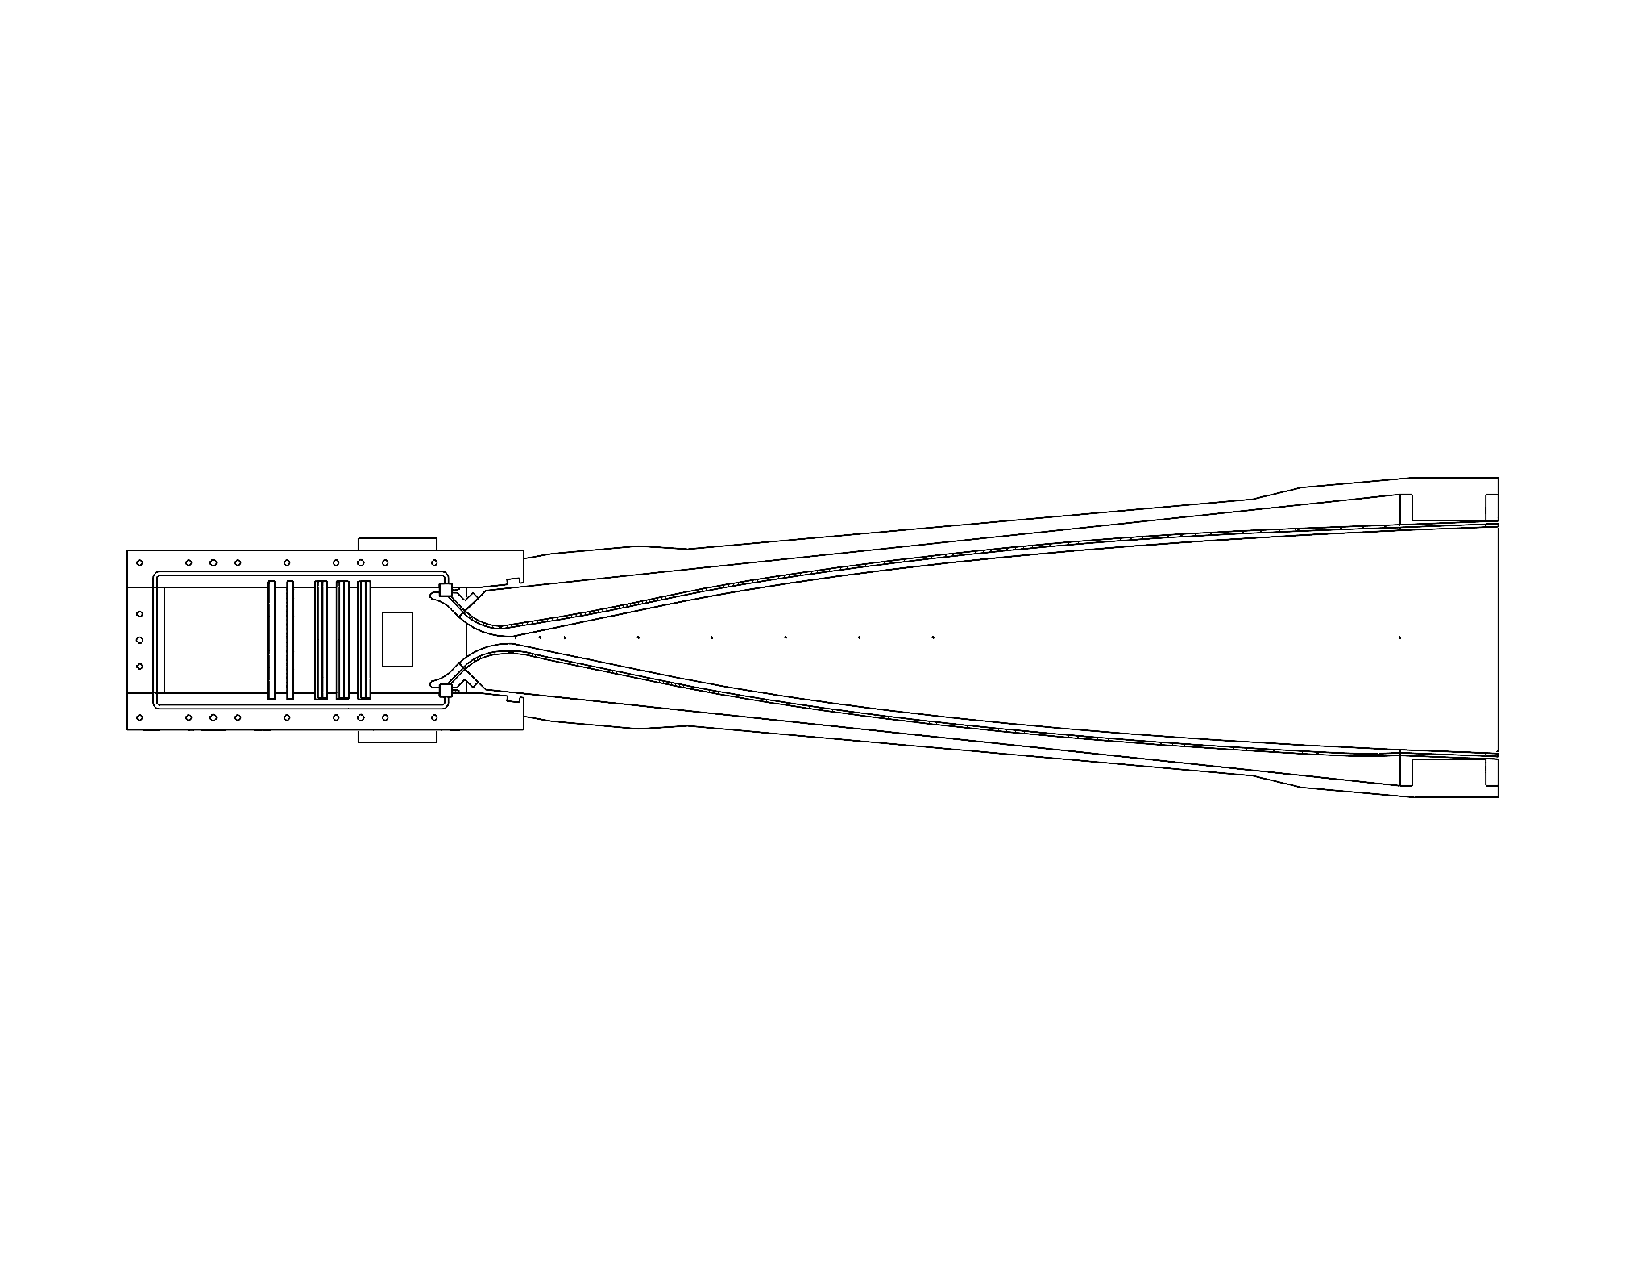
\includegraphics[trim={40 220 40 220},clip,width=6in]{ace-nozzle.pdf}
    \caption{ACE nozzle and settling chamber}
    \label{fig:ace-nozzle}
\end{figure}

The original motivation for the redesign was to remanufacture the nozzle to remedy the premature laminar-to-turbulent transition, which is discussed in the next section. However, as the redesign progressed, it became apparent that this was the best opportunity to completely redesign the nozzle and settling chamber to enable active control. This progression and the redesign process is detailed throughout this chapter.

\subsection{ACE Turbulent Transition}

ACE performance data \cite{aceturb,mai-dis,neel-dis,leidy-dis} shows that below a unit Reynolds number of $Re'$ = $\frac{\rho U}{\mu} \approx 3 \times 10^6/\mathrm{m}$ the RMS pressure fluctuations in the test section are less than 1\%, and that above this unit Reynolds number the pressure fluctuation levels significantly increase. It was desired to increase the unit Reynolds number at which laminar flow can be maintained, so the mechanism causing laminar-to-turbulent transition of the nozzle boundary layers had to be determined. The hypothesis and supporting data regarding the pressure fluctuation levels increase and how it might be delayed to higher unit Reynolds numbers is summarized below.

Five primary suspects for transition were identified:

\begin{enumerate}
    \item A known manufacturing surface discontinuity at the nozzle throat
    \item Sidewall mushroom vortices
    \item Görtler vortices
    \item Freestream turbulence in the incoming flow and/or upstream boundary layer
    \item Wall roughness or waviness
\end{enumerate}

The throat discontinuity (1) is the result of a decimal truncation error when connecting the subsonic curve to the supersonic MOC contour in Solidworks. The resulting discontinuity can be seen in Figure \ref{fig:ace-throat}, and it has a height of around 0.0003 inches. The artifact carried forward through the CNC machining and is present on the physical nozzle throat. \textcolor{red}{Is this a sufficient description?}

\begin{figure}[ht!]
    \centering
    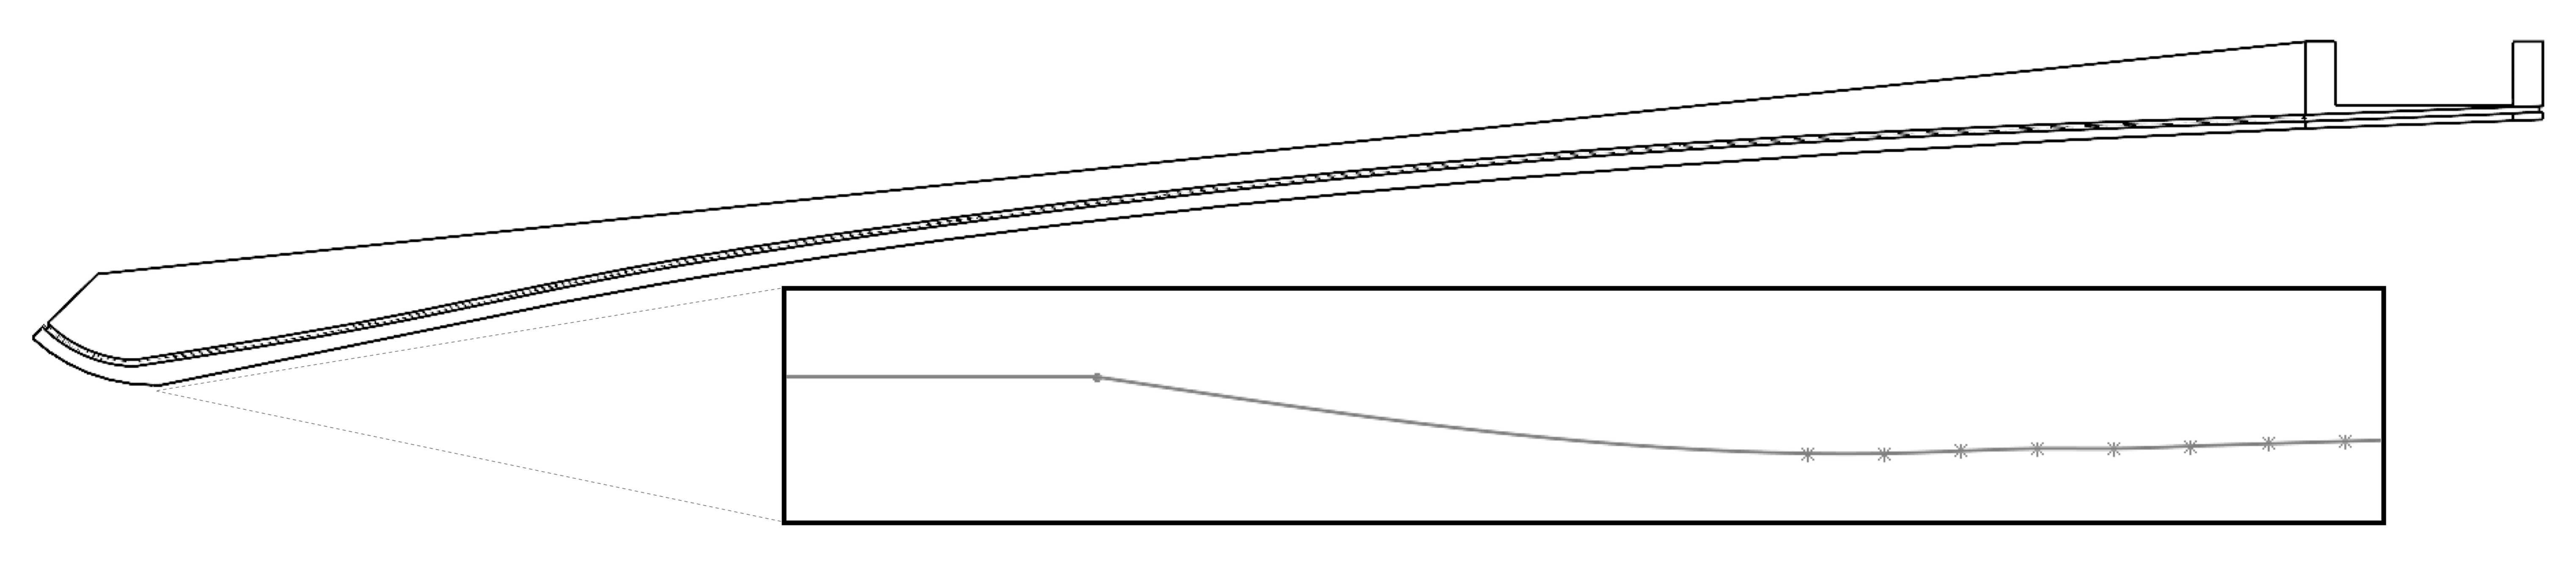
\includegraphics[width=6in]{ace-throat}
    \caption{ACE throat discontinuity}
    \label{fig:ace-throat}
\end{figure}


The sections below evaluate each of these possibilities and support the conclusion that the throat discontinuity is the most likely reason for the increased pressure fluctuations above $Re' \approx 3 \times 10^6/\mathrm{m}$. This conclusion is supported by pitot surveys, method-of-characteristics line tracing, and CFD simulations. Sidewall mushroom vortices (2) and Görtler vortices (3) would lead to transition too far downstream from the throat to be responsible for the pressure fluctuation levels increase. Incoming freestream turbulence (4) and wall surface quality (5) are potential causes of poor flow quality in all supersonic tunnels and are included for completeness. The specific mechanism by which these would cause transition is not known. While item 4 and 5 are not the primary suspects for the pressure fluctuation levels increase, improving these conditions will be addressed in the redesign intended to extend laminar flow to higher unit Reynolds numbers.

\subsubsection*{ACE Nozzle Noise Surveys}

Three recent pitot surveys have been conducted in the ACE tunnel. The first by Mai in 2014 \cite{mai-dis} revealed transition occurring around $Re' \approx 3 \times 10^6/\mathrm{m}$, as shown in Figure \ref{fig:mai-survey}. The same result was found by Neel in 2019 \cite{neel-dis} shown in Figure \ref{fig:neel-survey} that transition occurs at this $Re'$ value at a location 6 inches upstream of the nozzle exit. A final pitot survey in ACE by Wirth in 2022 (unpublished) was conducted to determine whether the pressure fluctuation levels increase occurred at different $Re'$ values at positions farther upstream in the nozzle. He found pressure fluctuation levels increase at $Re' \approx 3 \times 10^6/\mathrm{m}$ at a measurement location 17 inches upstream of the nozzle exit. His results in Figure \ref{fig:wirth-survey} align perfectly with Mai's and Neel's data and clearly establish that the Reynolds number at which pressure fluctuation levels increase is the same at all locations in the nozzle. This suggests that transition is not moving upstream through the nozzle as Reynolds number is increased.

\begin{figure}[ht!]
    \centering
    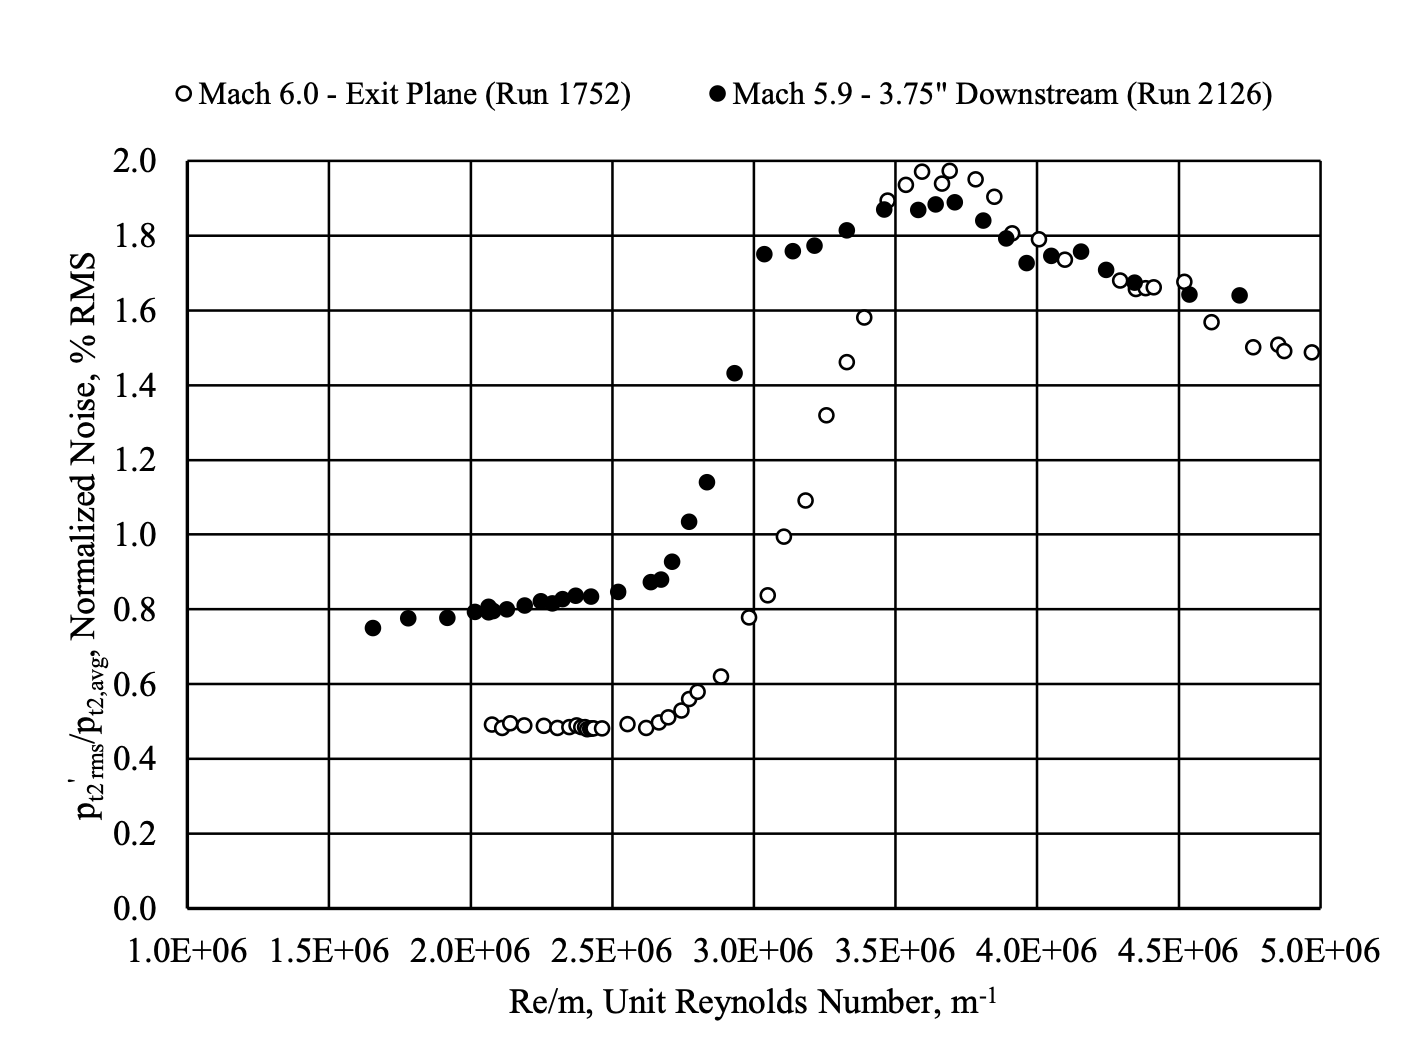
\includegraphics[width=5.5in]{mai-survey}
    \caption[ACE freestream pressure fluctuations in the nozzle exit plane as measured in 2014]{ACE freestream pressure fluctuations in the nozzle exit plane as measured in 2014 \cite{mai-dis}}
    \label{fig:mai-survey}
\end{figure}

\begin{figure}[ht!]
    \centering
    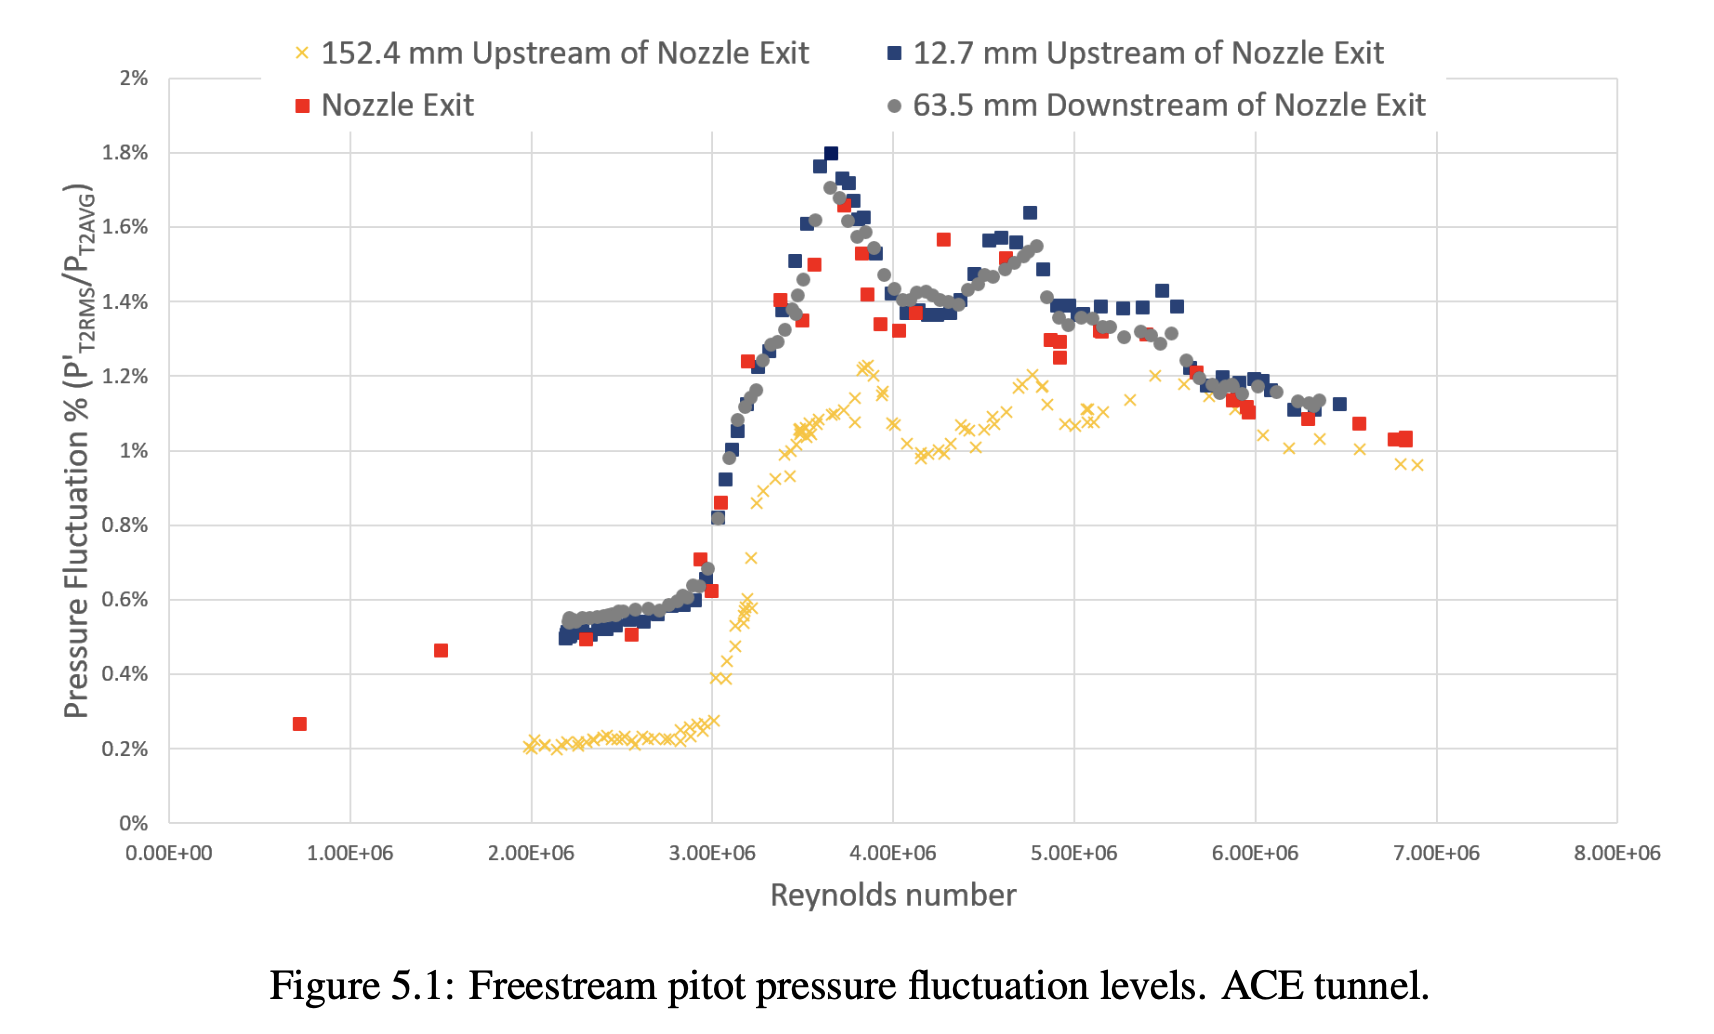
\includegraphics[width=6in]{neel-survey}
    \caption[ACE freestream pressure fluctuations at various locations as measured ii 2019]{ACE freestream pressure fluctuations at various locations as measured in 2019 \cite{neel-dis}}
    \label{fig:neel-survey}
\end{figure}

\begin{figure}[ht!]
    \centering
    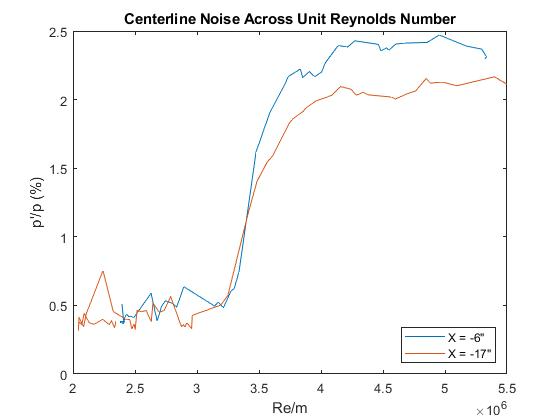
\includegraphics[width=5.5in]{wirth-survey}
    \caption{ACE freestream pressure fluctuations at 6 inches and 17 inches upstream of nozzle exit as measured in 2022}
    \label{fig:wirth-survey}
\end{figure}

\subsubsection*{Suspect Mechanism Conclusions}

The pressure fluctuation levels revealed the $Re'$ value at which transition occurs but not the transition mechanism. The two mechanisms that were extensively investigated at the start of this work were sidewall mushroom vortices and Görtler vortices. Sidewall mushroom vortices arise from the pressure distribution in the low momentum flow in the sidewall boundary layers. The flow at the centerline expands to the test section pressure ahead of the top and bottom curved walls. The flow at the top and bottom lags behind the centerline flow with a higher pressure to create a vertical pressure gradient that introduces a secondary vertical flow in the sidewall boundary layers that flows from the corners to the centerline \cite{sabnis}. CFD simulations by Kocian (unpublished) show the sidewall mushroom vortices beginning to form approximately 24 inches upstream of the nozzle exit shown in Figure \ref{fig:mushrooms}. 
\begin{figure}[ht!]
    \centering
    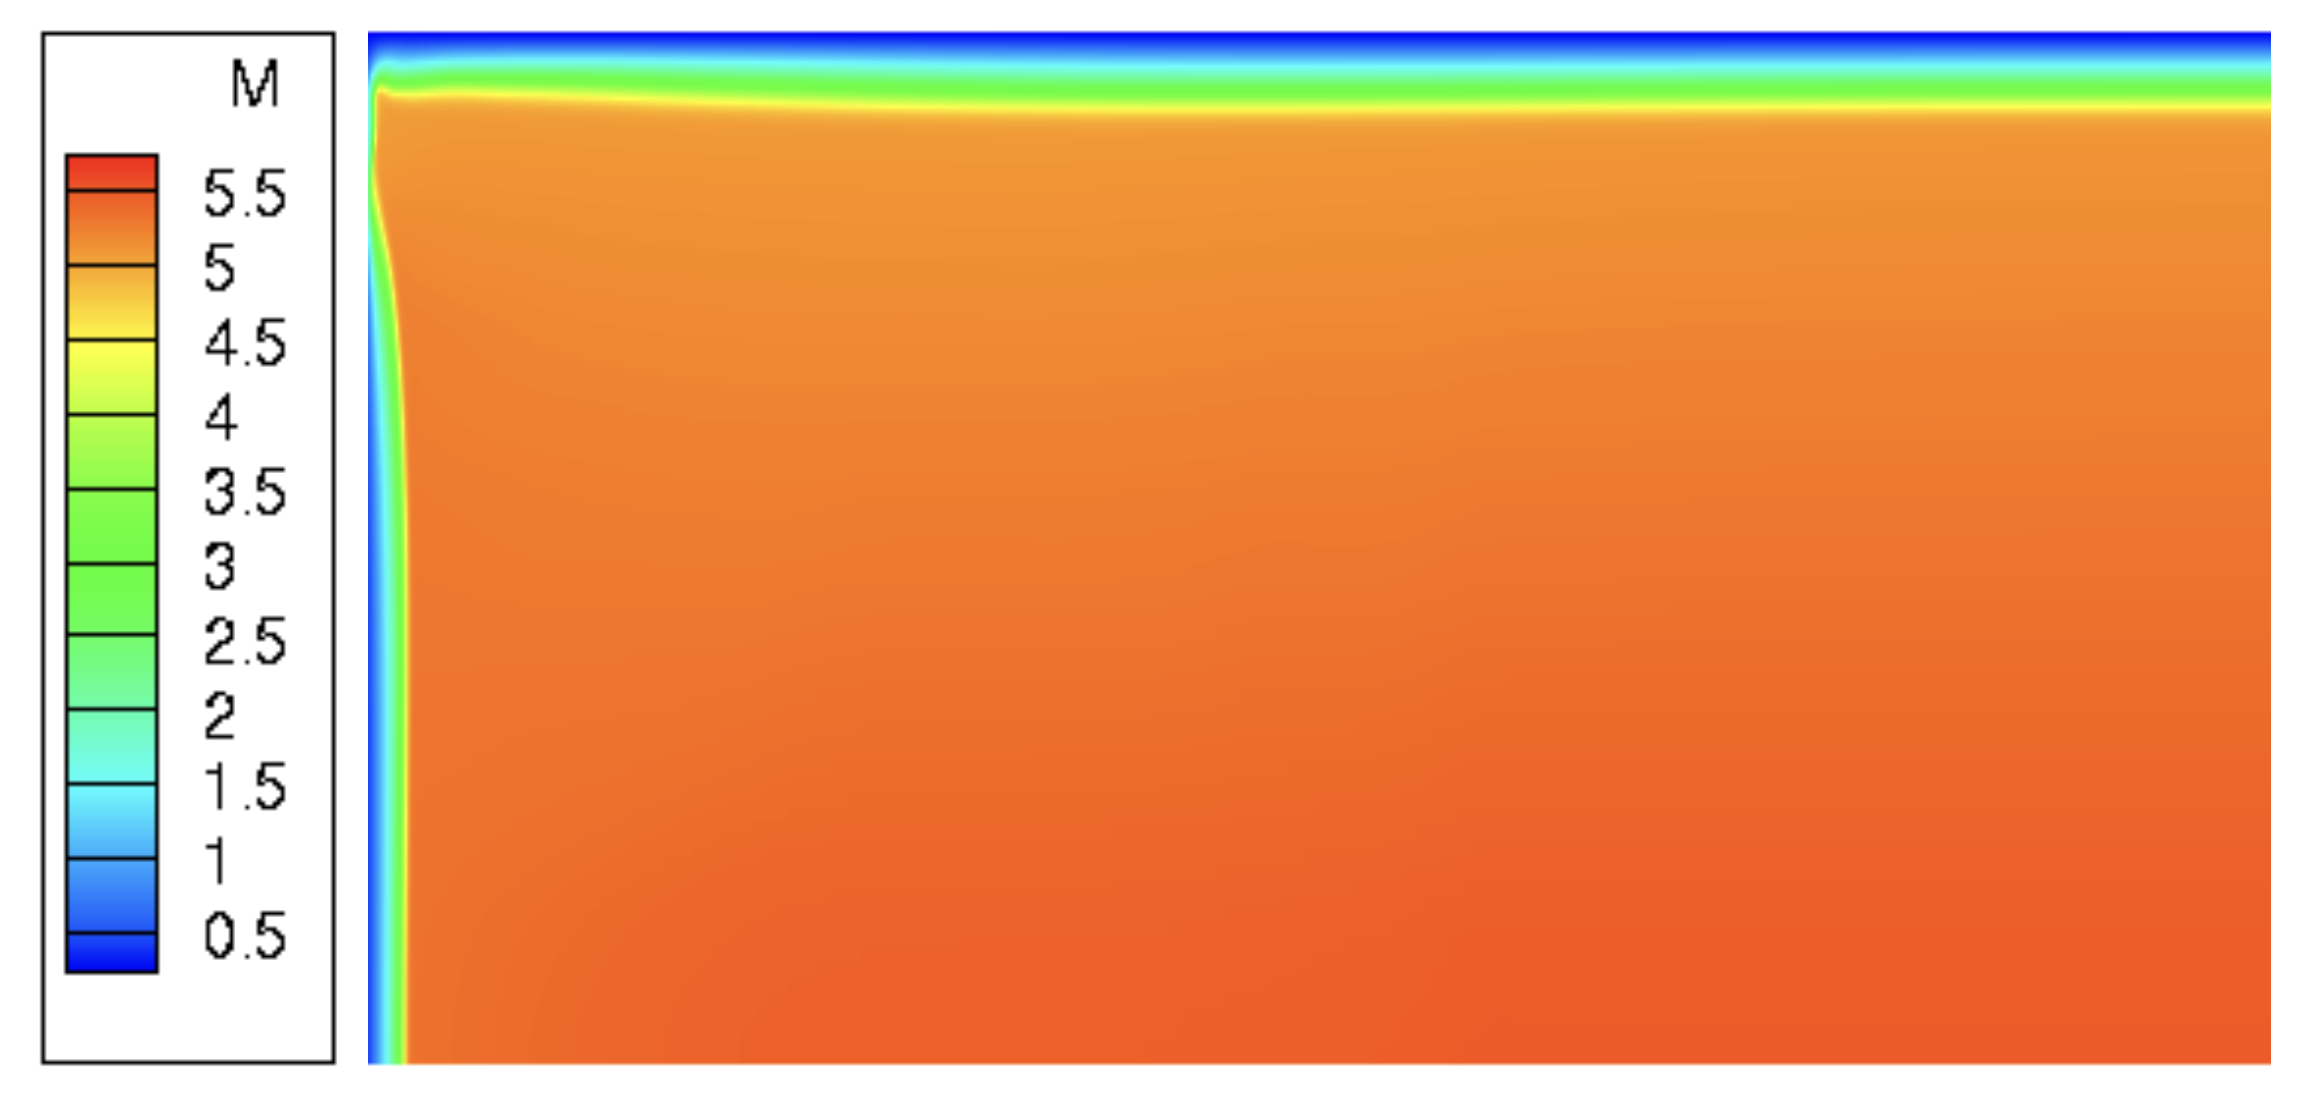
\includegraphics[width=5in]{mush24}
    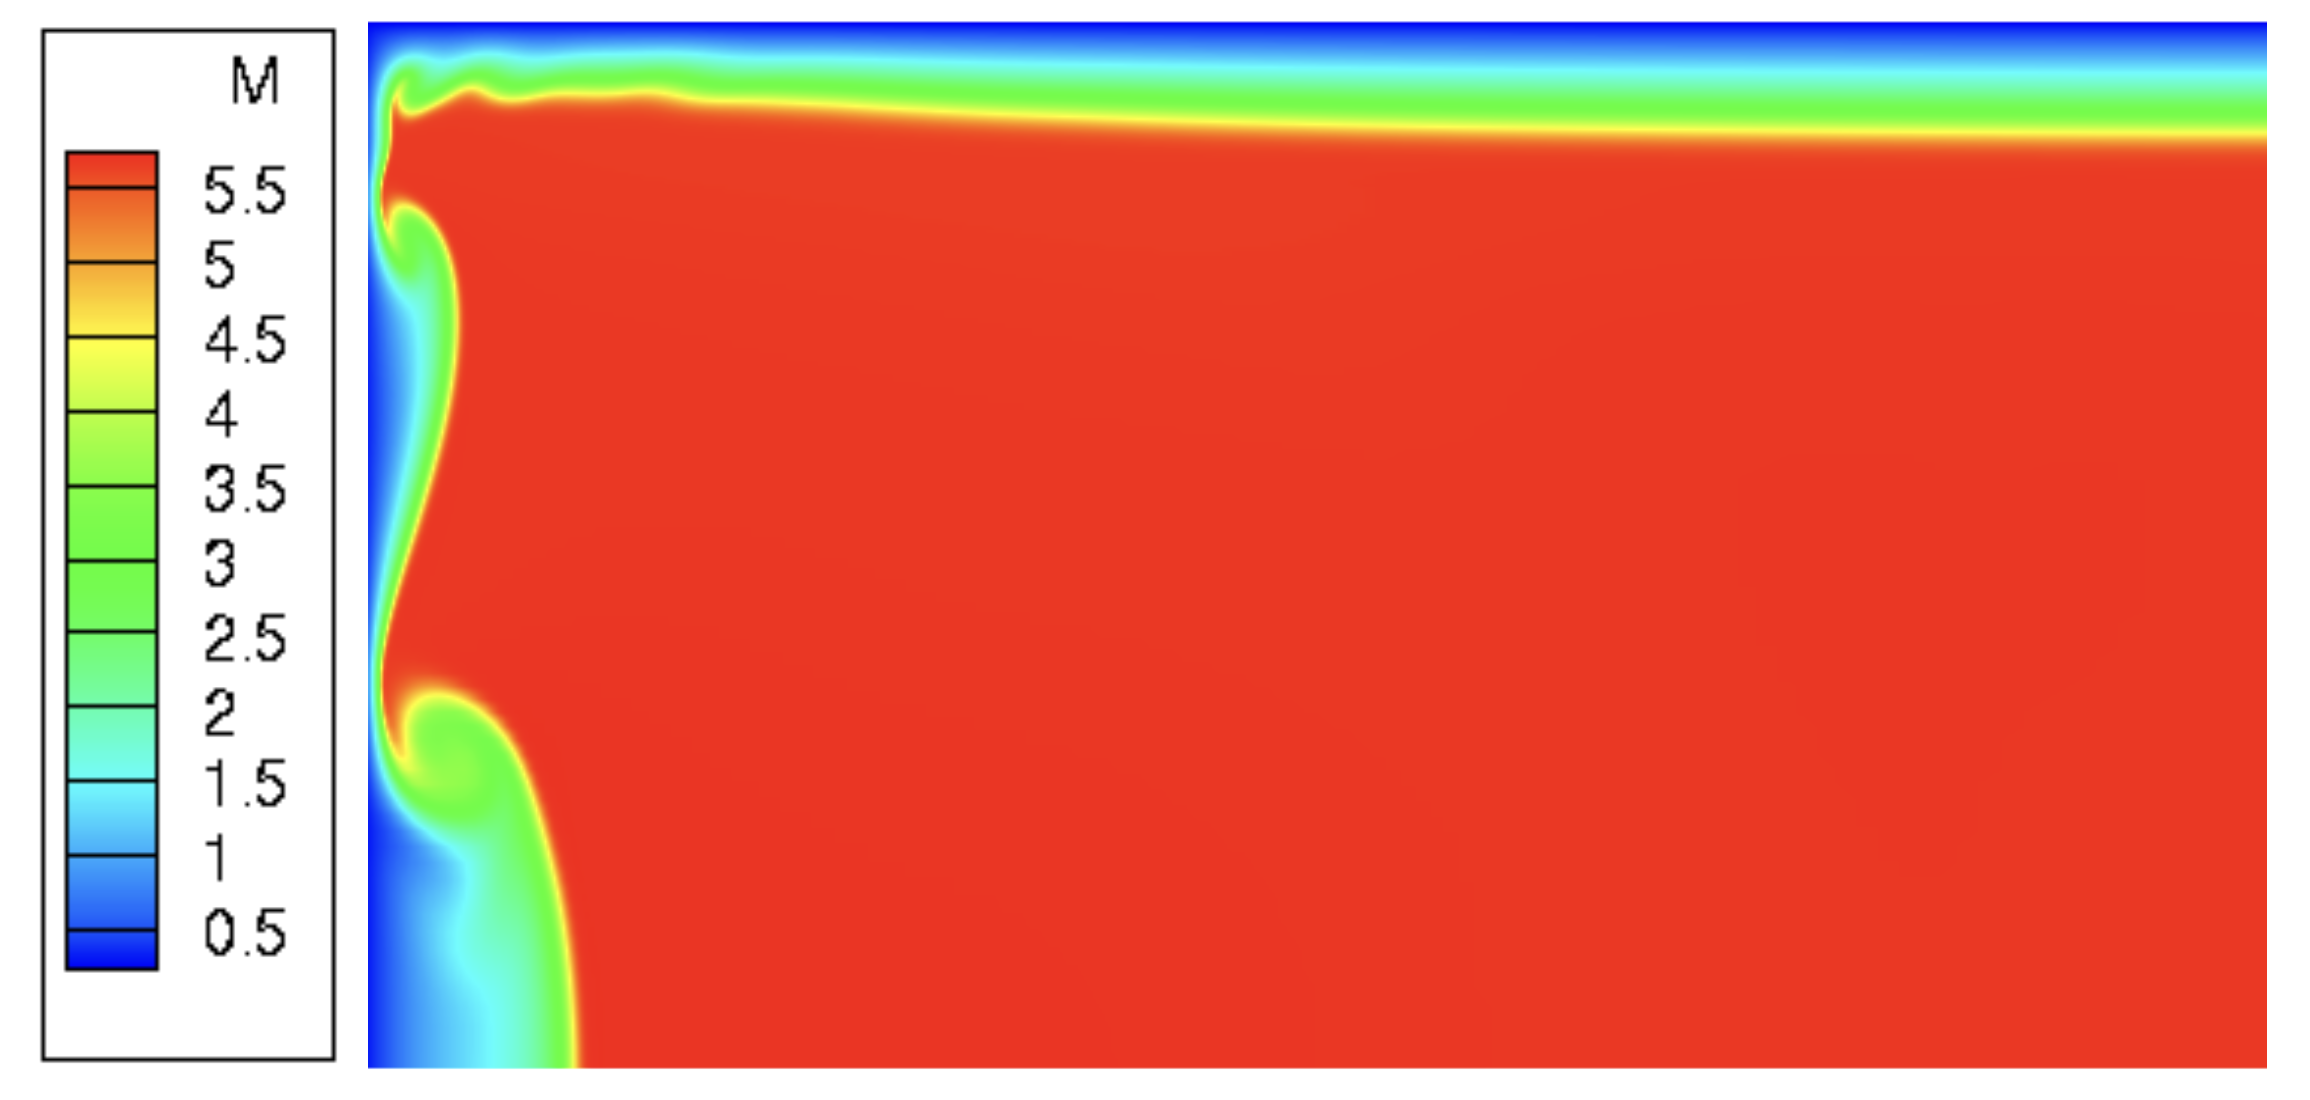
\includegraphics[width=5in]{mush0}
    \caption{Sidewall mushroom vortex formation (upper \textcolor{red}{quadrant/quarter}) at 24 inches upstream of nozzle exit (top) and at nozzle exit (bottom) }
    \label{fig:mushrooms}
\end{figure}

Görtler vortices are counter-rotating streamwise vortices that occur in boundary layers on concave surfaces \cite{saric}. To estimate where these may lead to transition, a CFD basic state simulation and N-factor analysis was performed by Kocian in 2022 (unpublished). The results, shown in Figures \ref{fig:gortler} and \ref{fig:n-factor}, indicate that Görtler vortices could induce transition around 8 inches from the nozzle throat. 

\begin{figure}[ht!]
    \centering
    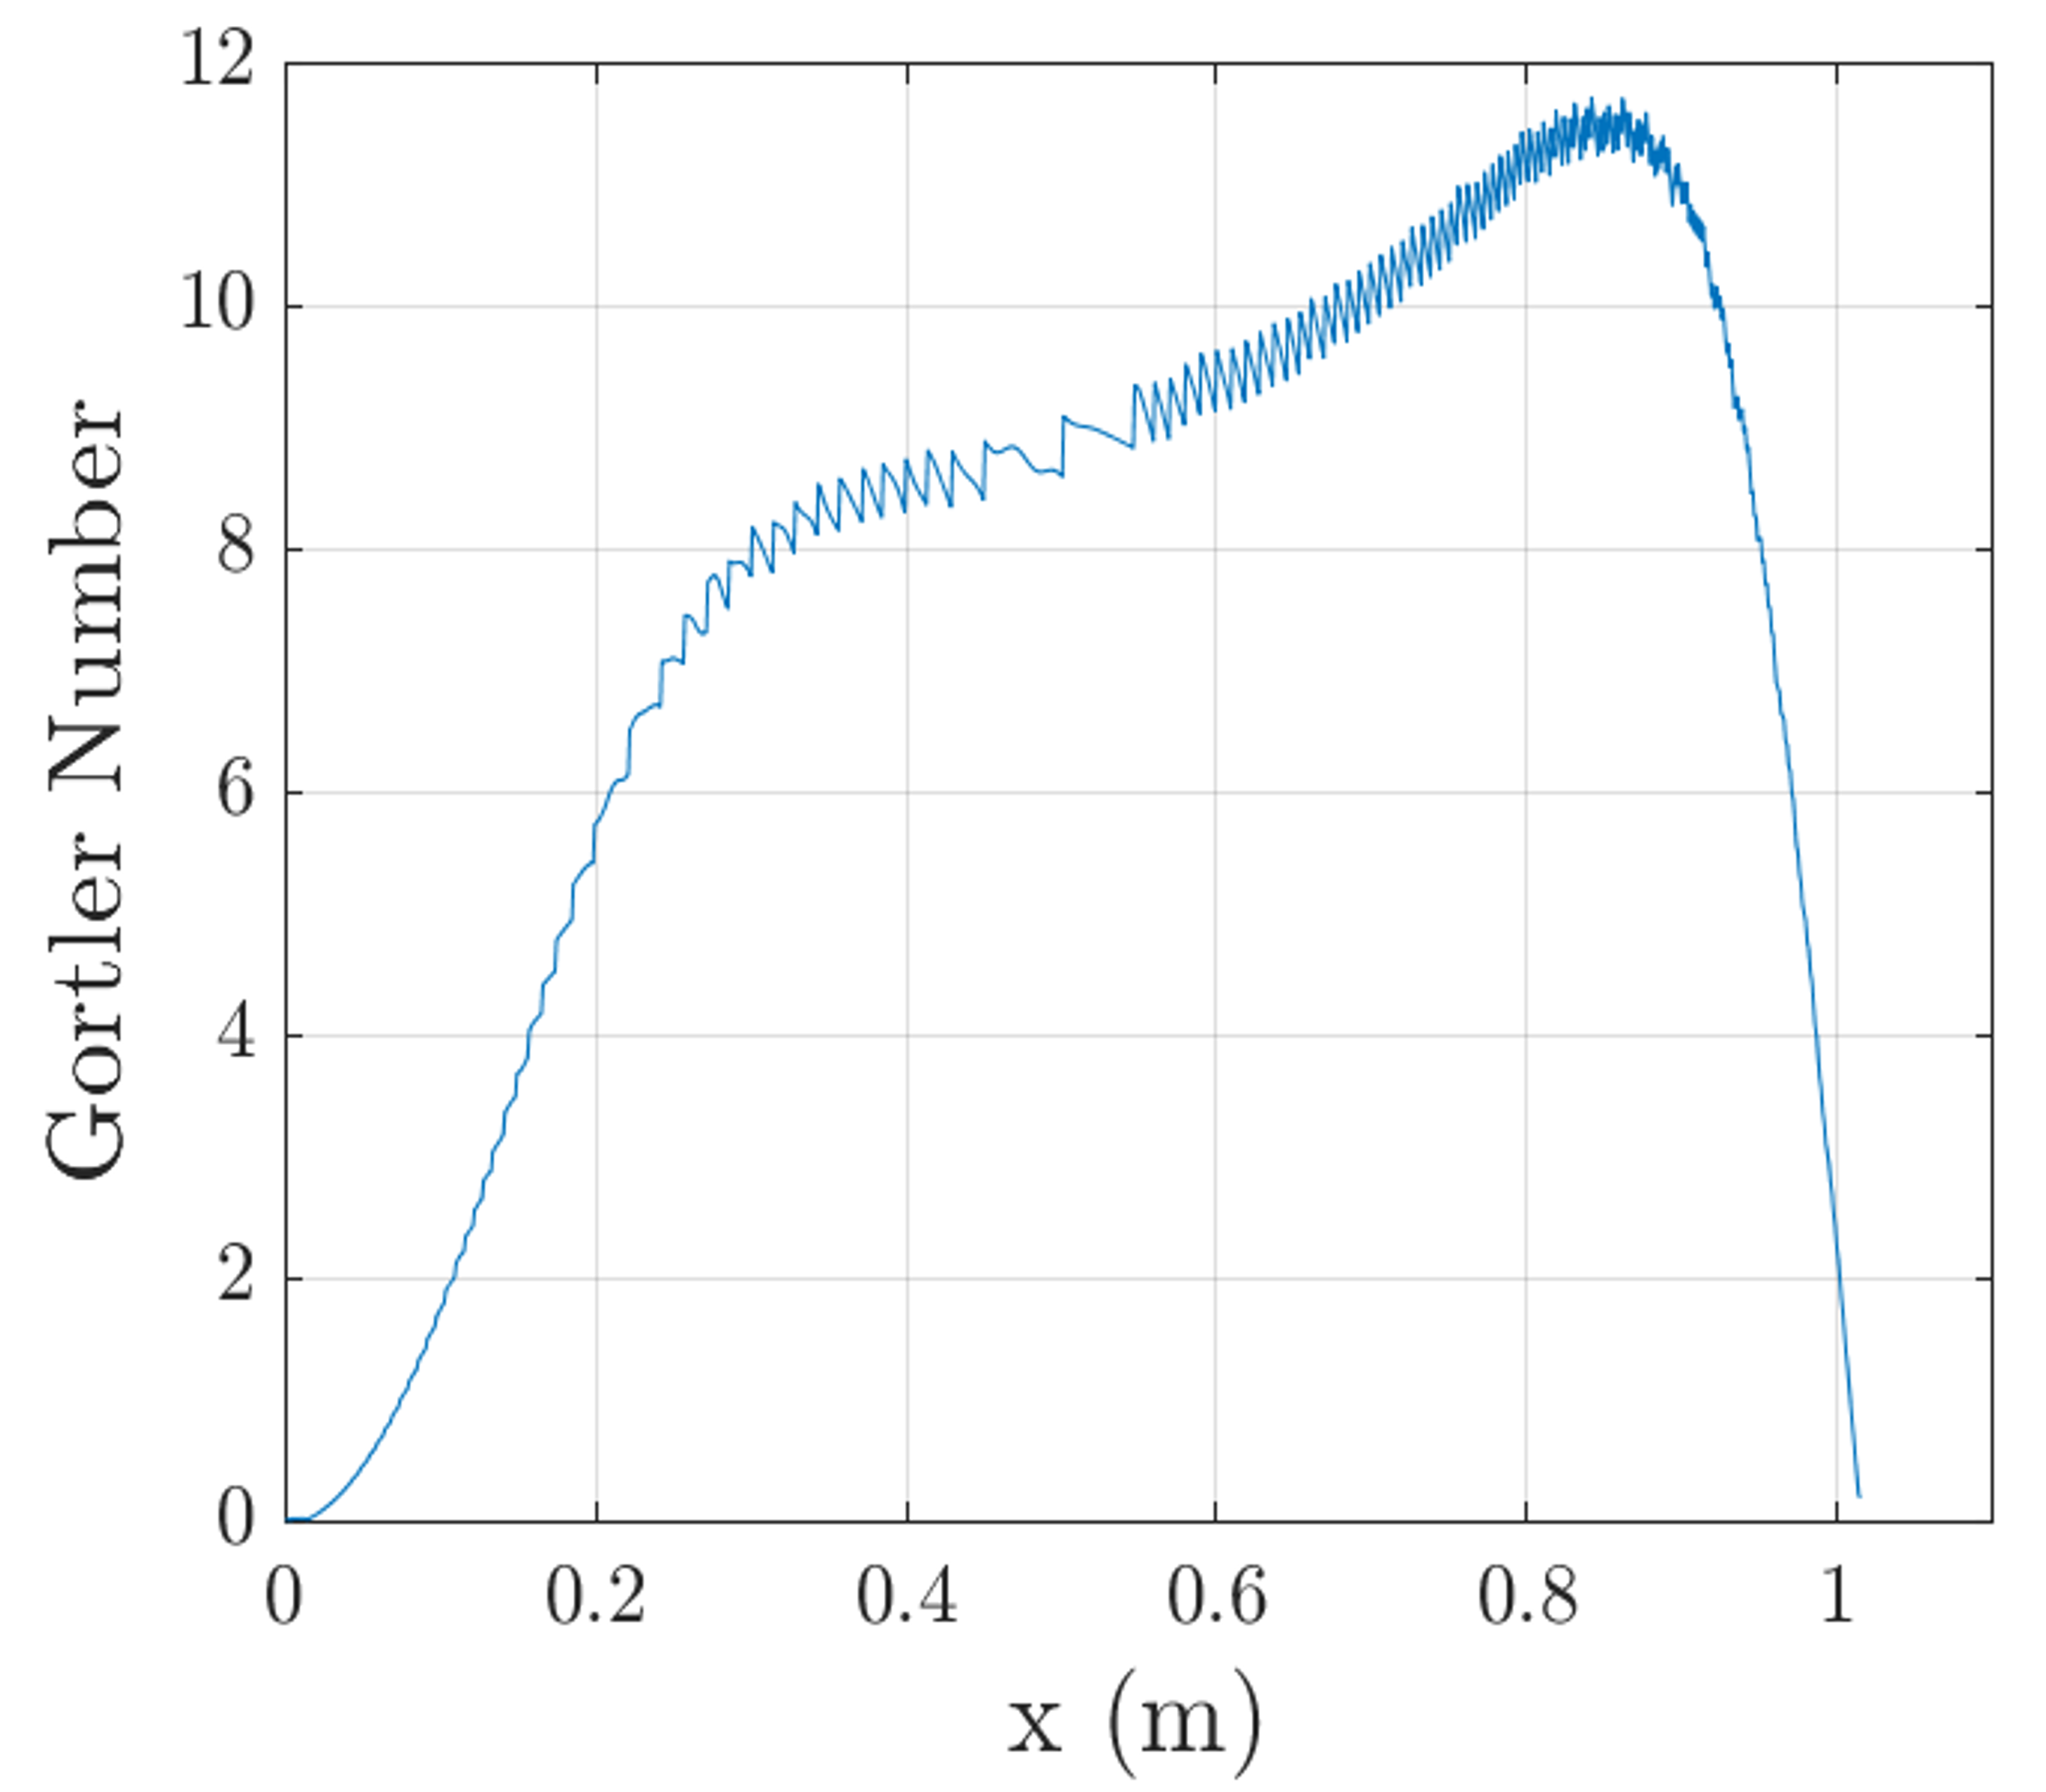
\includegraphics[width=5in]{gortler}
    \caption{Görtler number from ACE nozzle CFD}
    \label{fig:gortler}
\end{figure}

\begin{figure}[ht!]
    \centering
    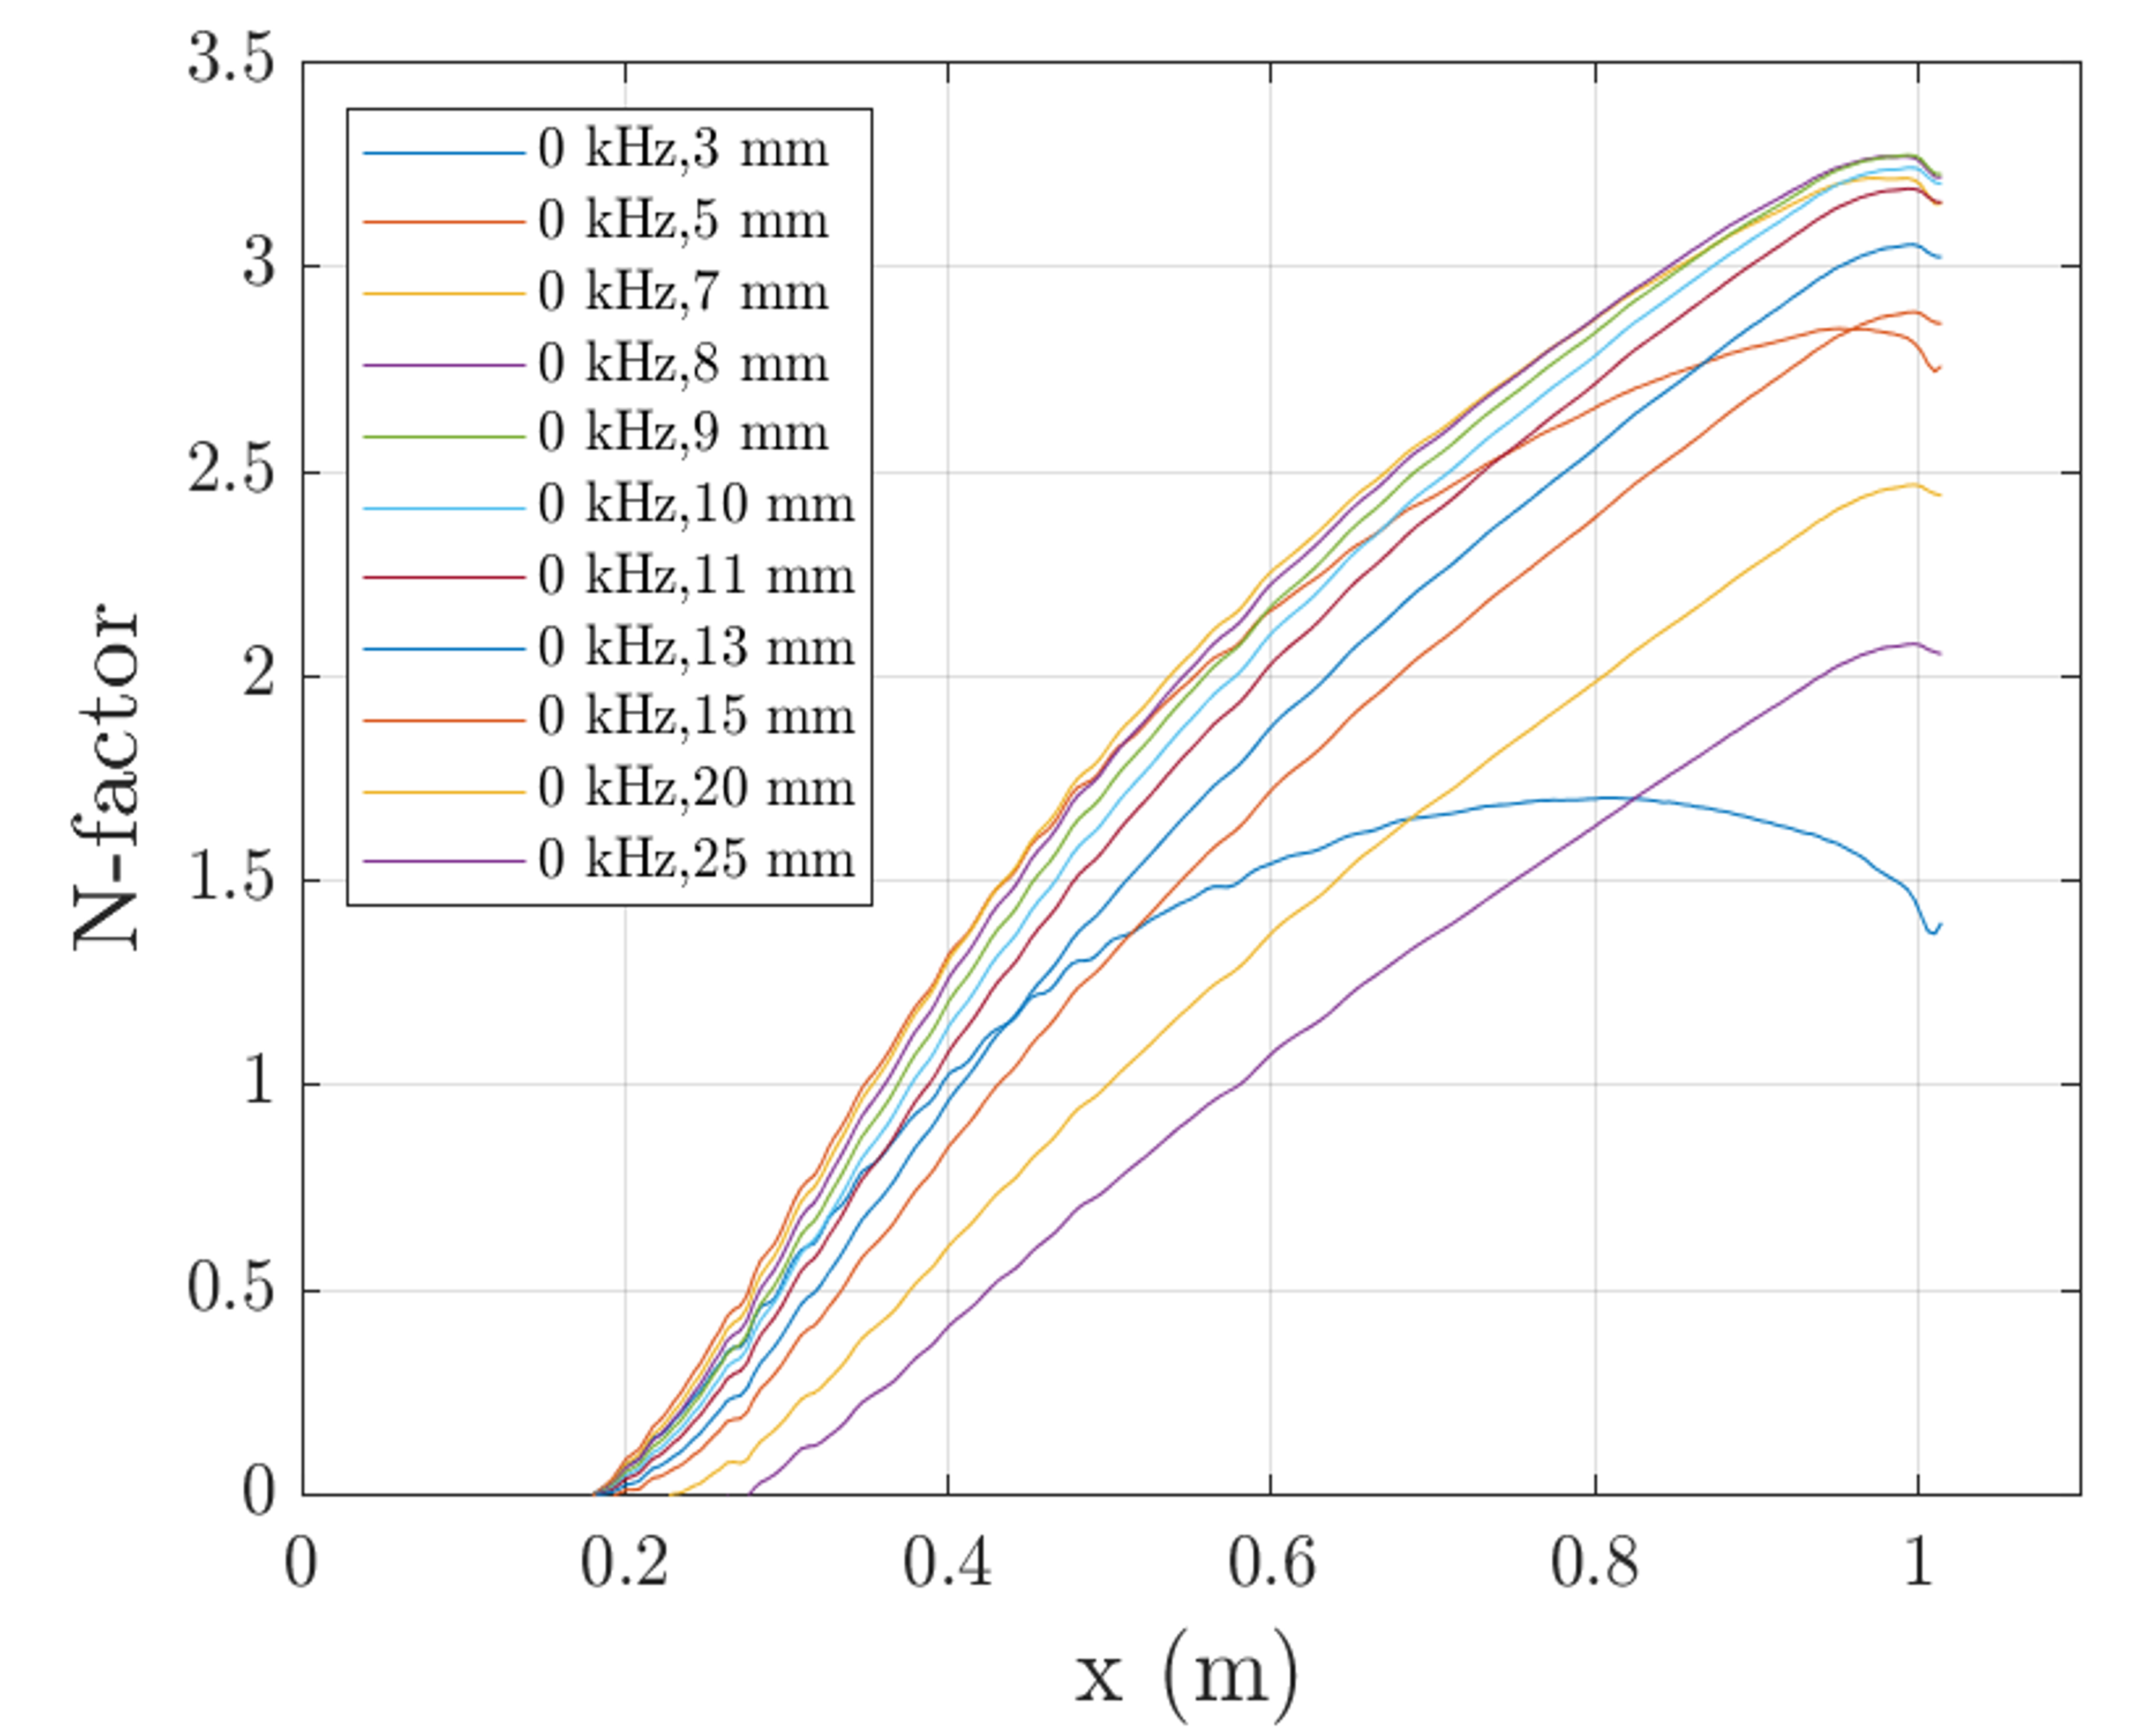
\includegraphics[width=5in]{n-factor}
    \caption{N-factors for Görtler number in ACE nozzle}
    \label{fig:n-factor}
\end{figure}

The origin of the noise measured farthest upstream of the nozzle exit was determined by tracing characteristic lines from the measurement location at the centerline upstream to the wall. Both the side view and top view of this can be seen in Figure \ref{fig:machlines}. This was accomplished by choosing the characteristic output by the MOC code that intersects the centerline closest to the measurement point of 17 inches and tracing it back to its origin at the wall. The measured noise origin from the top view is upstream of the throat where sidewall mushroom vortices are not relevant, and the origin is near the end of the straight section of the nozzle where Görtler has not had sufficient time to induce transition. While both sidewall vortices and Görtler vortices can play some role in transition in planar nozzles, they are no longer considered suspects for the pressure fluctuation levels increase at unit Reynolds numbers above $3 \times 10^6/\mathrm{m}$.

\begin{figure}[ht!]
    \centering
    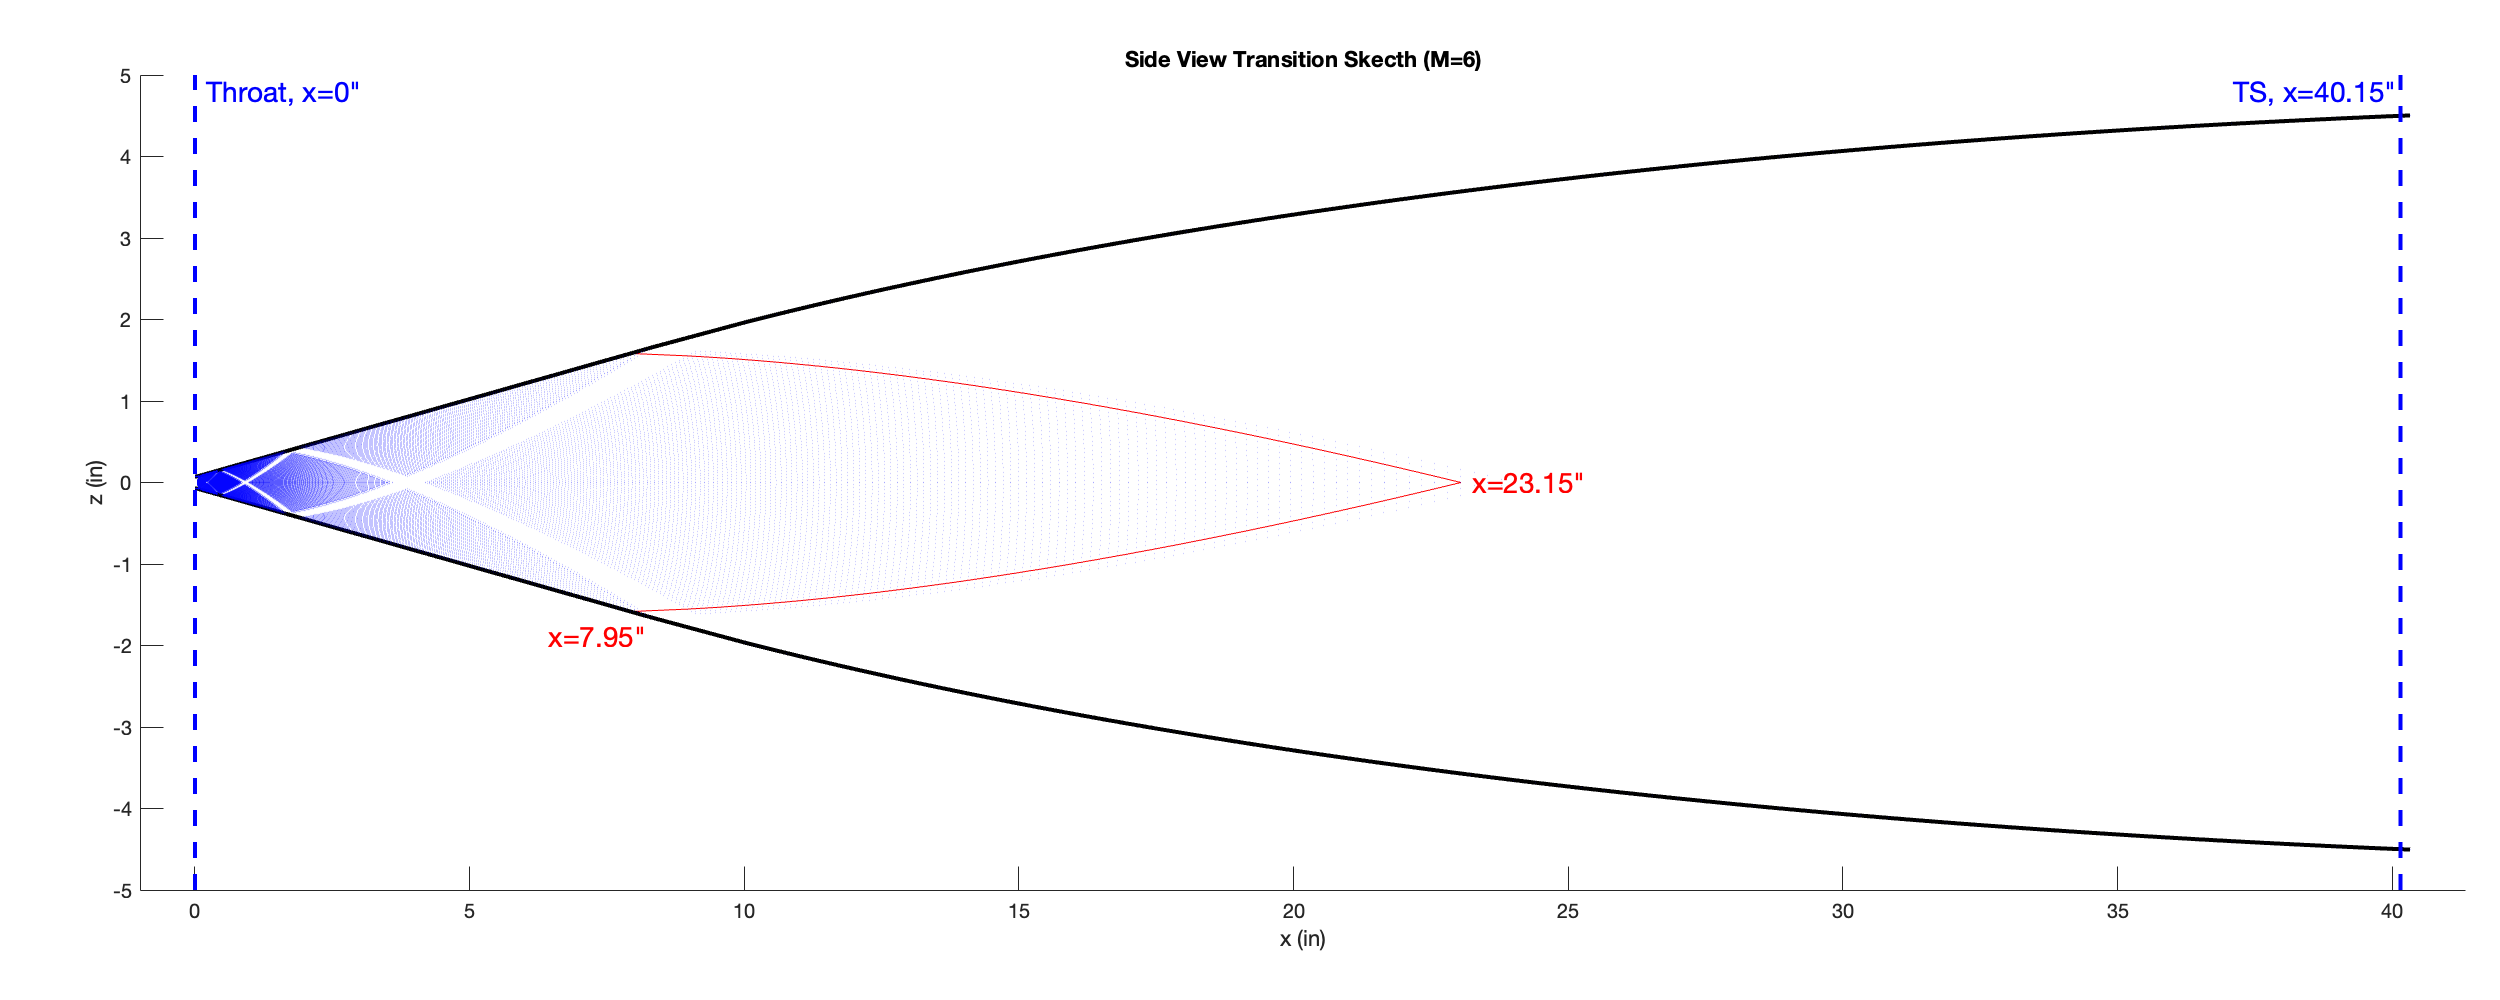
\includegraphics[width=6.5in]{side17}
    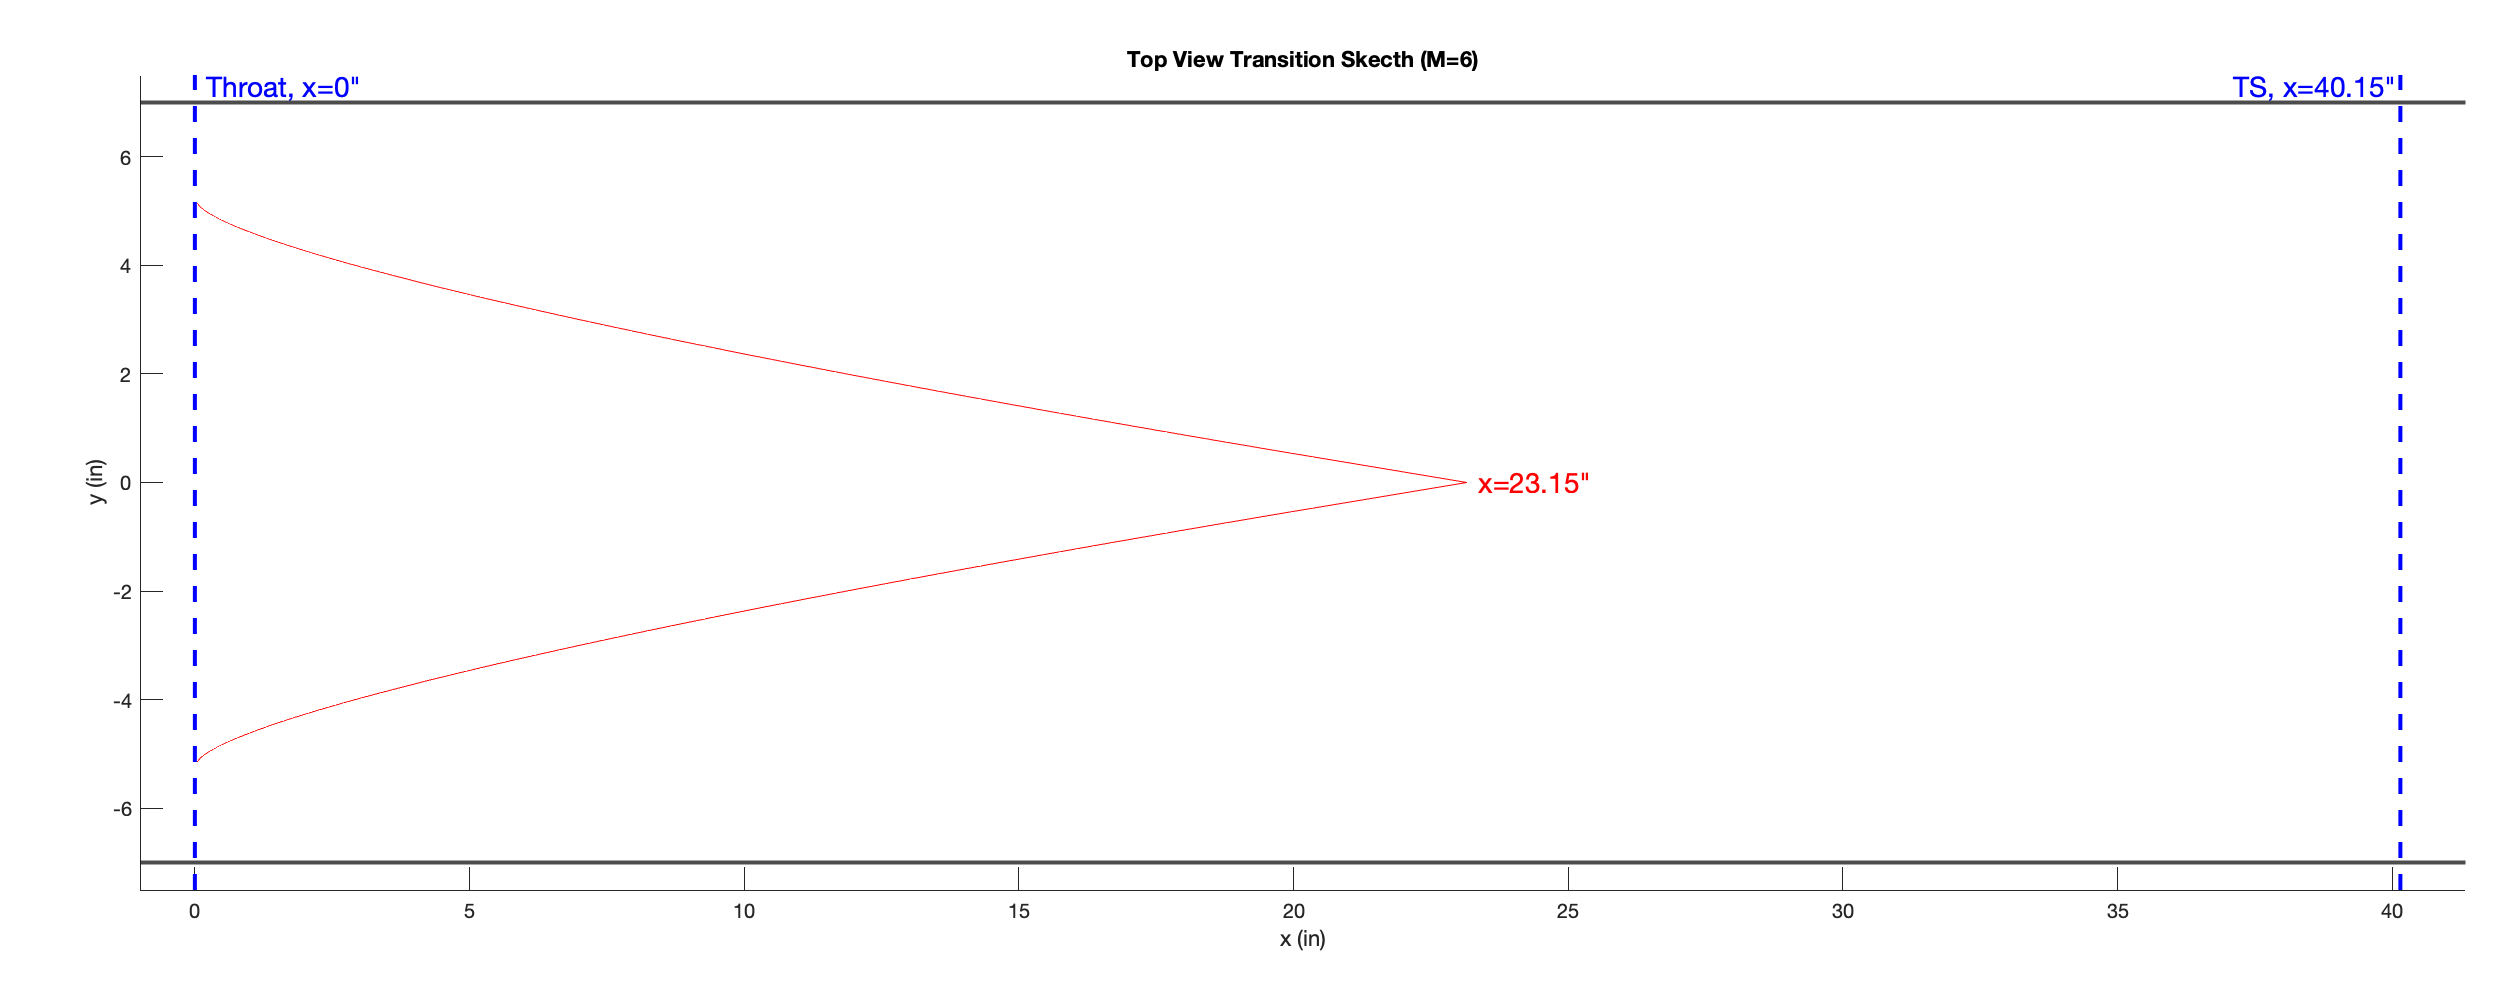
\includegraphics[width=6.5in]{top17}
    \caption{Mach lines for noise measured at 17" upstream on nozzle exit.}
    \label{fig:machlines}
\end{figure}

Following the above conclusions and recommendations, the most likely reason the pressure fluctuations increase is laminar-to-turbulent transition due to a surface discontinuity at the throat. This conclusion is supported by pitot surveys, CFD, and method of characteristics line tracing described above. The remaining suspect mechanisms are still important to note and address in the redesign of the ACE tunnel. 

\subsubsection*{Design Recommendations}

The following improvements are recommended to maintain laminar flow above $Re'$ $\approx 3 \times 10^6/\mathrm{m}$:
\begin{enumerate}
    \item Second-derivative-smooth subsonic-to-supersonic throat transition to eliminate nozzle throat discontinuity
    \item Continuous curvature with analytical functions to eliminate waviness and surface discontinuities
    \item Enhanced surface polishing to minimize surface roughness
    \item Improved settling chamber design to maximize flow uniformity and minimize freestream turbulence upstream of the nozzle throat
\end{enumerate}

One recommendation that is outside the scope of this work is to incorporate subsonic boundary layer suction to greatly reduce the incoming noise and potentially make ACE2.0 a "quiet" facility. Boundary layer suction is quite complex to effectively implement, but it will be accommodated for in the design in case it is explored in the future. 

\section{ACE2.0 Design}

Following these recommendations, the nozzle will be redesigned and remanufactured to meet specific requirements that will ensure the best performance and potentially expand the laminar Reynolds number range. The decision to remanufacture the nozzle presents an opportunity to revise the nozzle and settling chamber design to achieve true active controllability, properly embodying the "ACE" name.

The rest of the chapter details the planned improvements to the ACE tunnel and specific design requirements that will achieve those improvements. In addition to a new nozzle, the settling chamber will also be redesigned to ensure the uniformity and reduce the turbulence of the flow into the nozzle. These improvements are to achieve the goal of increasing the unit Reynolds number at which laminar nozzle flow is maintained.

\subsection{Design Requirements}

ACE2.0 will maintain many characteristics while improving some, so many requirements are the same as the original ACE design. The new tunnel will still produce uniform Mach 5 to 8 flow in the 9 inches by 14 inches test section, withstand a total temperature of 530 K, and maintain a minimum engineering factor of safety (FOS) of 1.5 when operating at a total pressure of 200 psia.

\subsubsection*{Nozzle Requirements}

The current ACE nozzle successfully produces uniform Mach 5 to 8 flow in its core. In order to maintain this good performance and not introduce unknown parameters, the new nozzle will retain a very similar contour with slight improvements. The requirements that remain the same are that the nozzle must produce uniform flow for the entire Mach range, achieve maximum height deflection without exceeding a FOS of 1.5, and prevent leaks up to 200 psia.

The improvements to the nozzle and associated requirements will be a contour with continuous 1st and 2nd derivatives that is specified by analytical functions that will eliminate discontinuities and truncation error and a maximum allowable stress less than or equal to that found in the current ACE flexure at maximum deflection.

\subsubsection*{Settling Chamber Requirements}

The current ACE settling chamber design provides multiple opportunities to improve flow conditioning and ease of maintenance. The new settling chamber design will increase the length and height and allow for variable aerogrid/screen configurations. The requirements that remain the same are low freestream turbulence, thin stable wall boundary layers, maximum uniformity, and preventing leaks at a pressure of 200 psia. The implementation of these requirements will be improved in the new design to achieve improved incoming flow into the nozzle.

Following Reshotko et al. \cite{reshotko}, the length of the settling chamber shall accommodate a separation of 250 characteristic mesh sizes between screens allowing for adequate turbulence decay. The aerogrids will have a hexagonal perforation pattern to increase porosity and decrease pressure loss. The number of aerogrids and screens shall be variable to allow for future flow conditioning experiments. The inlet shall include a baffle system that will provide an acceptable initial distribution and mixing of the air received from the high-pressure inlet piping. The overall design will accommodate the option for future boundary layer suction slots.

A settling chamber height of 6 inches was chosen to keep the velocity as slow as possible without going below 10 ft/s for the majority of the Mach number range, according to Pope and Goin \cite{pope}. The reason for this minimum is to prevent thermal convection vortices from dominating the flow at the walls. The interior of ACE2.0 will also be heated prior to the start of the run to help avoid thermal gradients. 

% With this in mind, the height of 6 inches was chosen as a good compromise as seen in Table \ref{tab:sc_vel}.

% \begin{table}[ht!]
%     \centering
%     \begin{tabular}{|c|c|c|c|c|}
%         \cline{2-5}
%         \multicolumn{1}{c}{} & \multicolumn{4}{|c|}{\textbf{Mach Number}} \\ \hline
%         \textbf{Height} & 5 & 6 & 7 & 8 \\ \hline
%         4" & 73.57 & 34.55 & 17.64 & 9.66 \\ \hline
%         5" & 58.83 & 27.64 & 14.11 & 7.73 \\ \hline \hline
%         6" & 49.01 & 23.03 & 11.76 & 6.44 \\ \hline \hline
%         7" & 42.00 & 19.74 & 10.08 & 5.52 \\ \hline
%         8" & 36.75 & 17.27 & 8.82 & 4.83 \\ \hline
%         9" & 32.66 & 15.35 & 7.84 & 4.29 \\ \hline
%     \end{tabular}
%     \caption{Settling chamber velocities (ft/s) for combinations of settling chamber heights and Mach numbers.}
%     \label{tab:sc_vel}
% \end{table}
    
\subsection{Nozzle Contour Codes}

The multiple reflections method-of-characteristics (MOC) Fortran script written by Bowersox that produced the ACE nozzle contour was used for the new nozzle contour. In order to achieve continuous first and second derivative continuity, a section of the code was modified to produce a fourth-order expansion section instead of the original second-order curve. This allowed the expansion section to match the curvature of both the subsonic section and the straight section. The code modification is included in Appendix \ref{appendix:contour}, and a comparison of the original quadratic and the new quartic expansion sections is shown in Figure \ref{fig:throats}. In this figure, the ACE contour is directly from the MOC points and the ACE2.0 contour is specified by an analytic fourth-order polynomial. The waviness of the MOC points can be seen here, emphasizing the need to define the entire nozzle with analytic functions.

\begin{figure}[ht!]
    \centering
    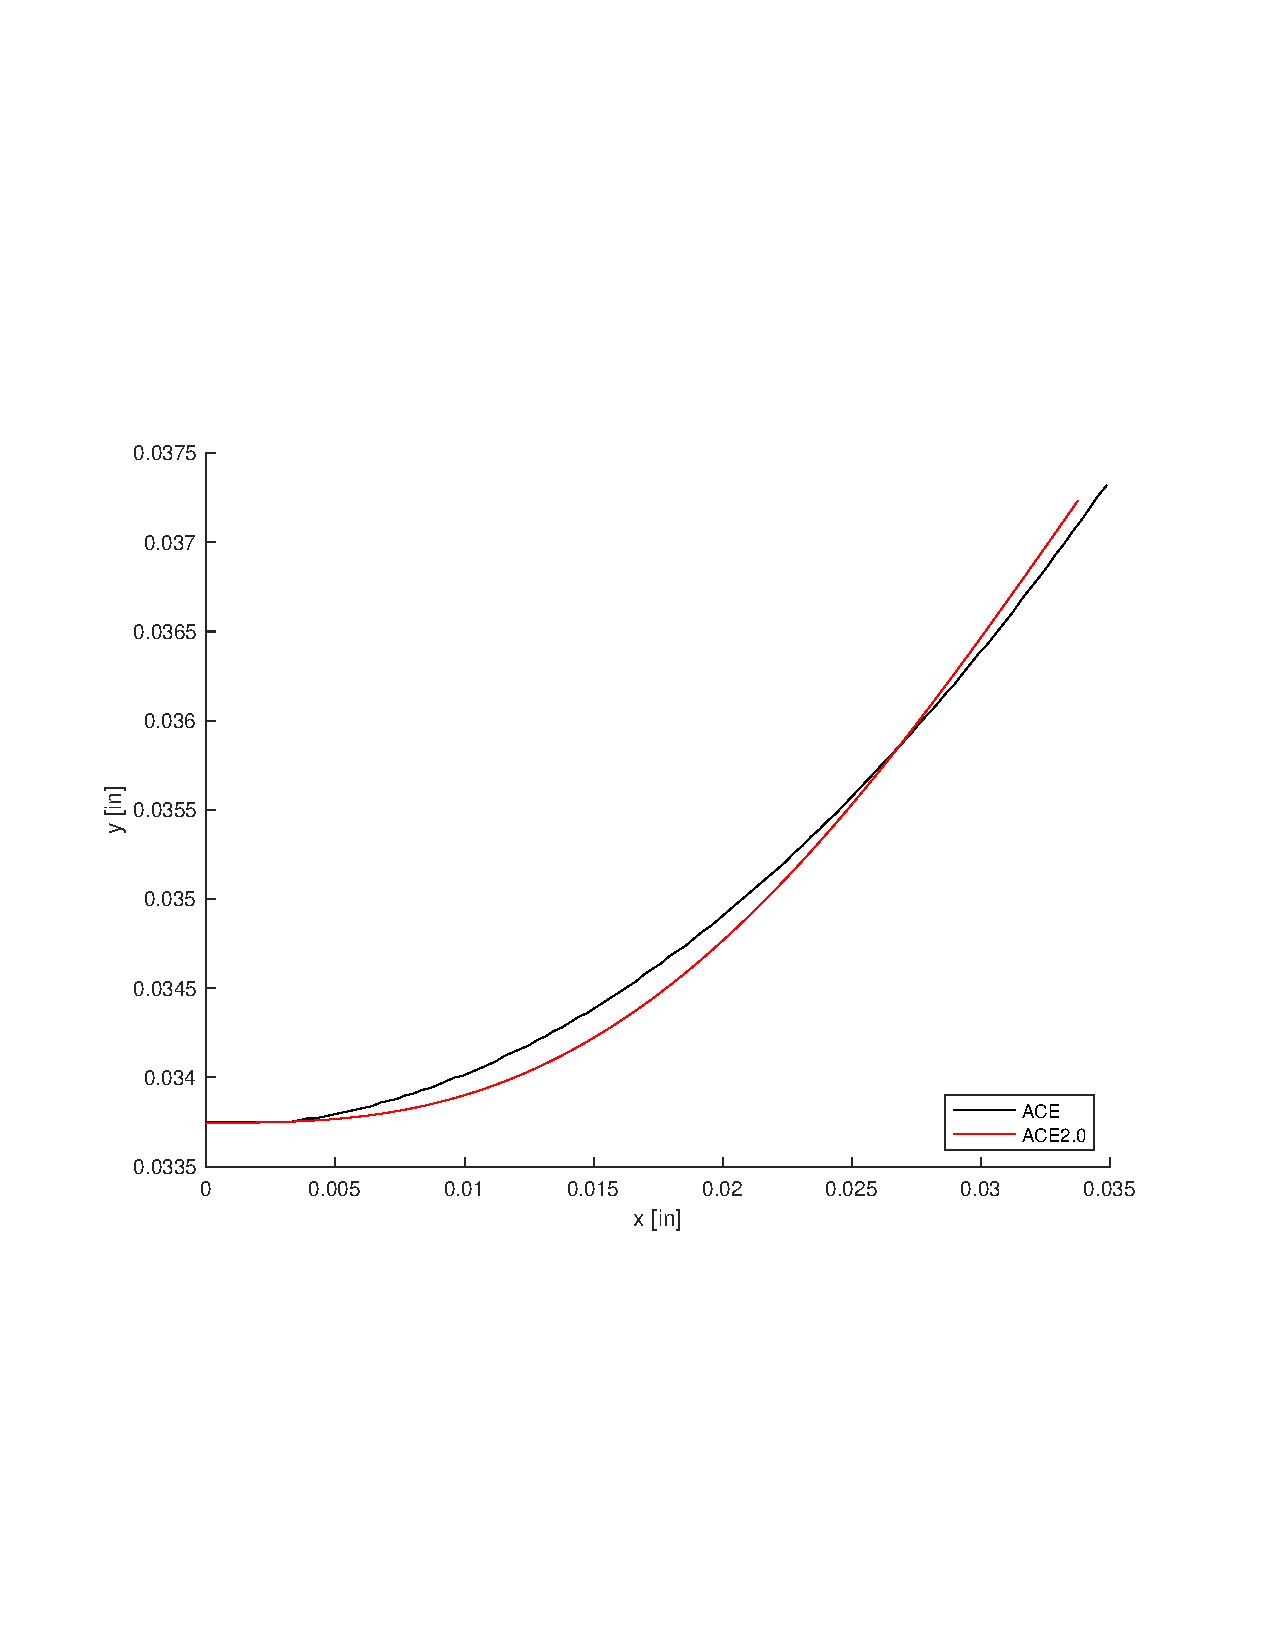
\includegraphics[trim={50 200 50 200},clip,width=6in]{throats.pdf}
    \caption{Comparison of ACE (quadratic) and ACE2.0 (quartic) expansion at throat}
    \label{fig:throats}
\end{figure}

After the MOC points were produced by the Fortran script, they were imported into a MATLAB script to fit with analytic functions. The subsonic curve is given by a fifth-order polynomial with six boundary conditions of the settling chamber and throat heights and zero slope and curvature at both the start and throat. The straightening section is given by a function found using the \texttt{lsqcurvefit} function with a combination of power and logarithmic functions in MATLAB. The equations for each section are given in Appendix \ref{appendix:contour}.

\subsection{CFD}

In order to verify the above nozzle contour performance compared to the original ACE contour, both contours were simulated in 2D CFD. First, a mesh was created in Pointwise for each contour with 400 equally spaced columns of cells in the x-direction. Each column had the spacing scaled to accurately capture the boundary layer with the smallest cell height around $4 \times 10^{-6}$ inches at the curved wall and the largest around 0.2 inches at the centerline as seen in Figure \ref{fig:mesh}. The CFD analysis was performed at a time when the settling chamber design was still at a height of 9 inches, so the analysis will be performed again to validate the 6 inch.

\begin{figure}[ht!]
    \centering
    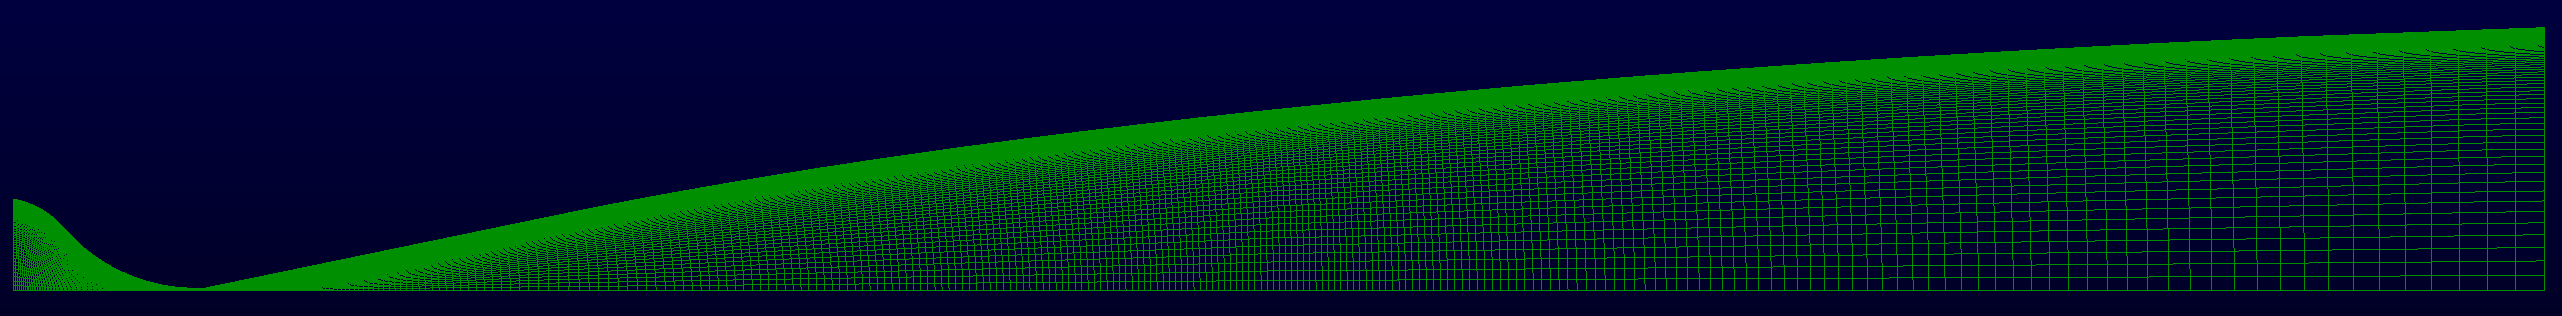
\includegraphics[width=6in]{ace-mesh}
    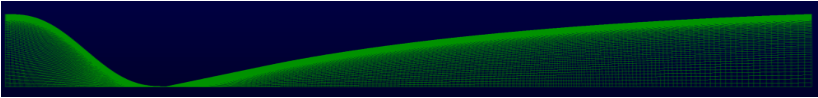
\includegraphics[width=6in]{qace-mesh}
    \caption{Mesh in Pointwise for ACE (top) and ACE2.0 (bottom) nozzle contours}
    \label{fig:mesh}
\end{figure}

After creating a mesh for each, they were simulated using US3D on the Texas A\&M supercomputer, Grace. \textcolor{red}{Stuff about inputs and convergence conditions...} A sample of the results is shown in Figure \ref{fig:ace2-cfd}. The full ACE2.0 CFD input conditions and results compared to ACE is given in Appendix \ref{appendix:cfd}.

\begin{figure}[ht!]
    \centering
    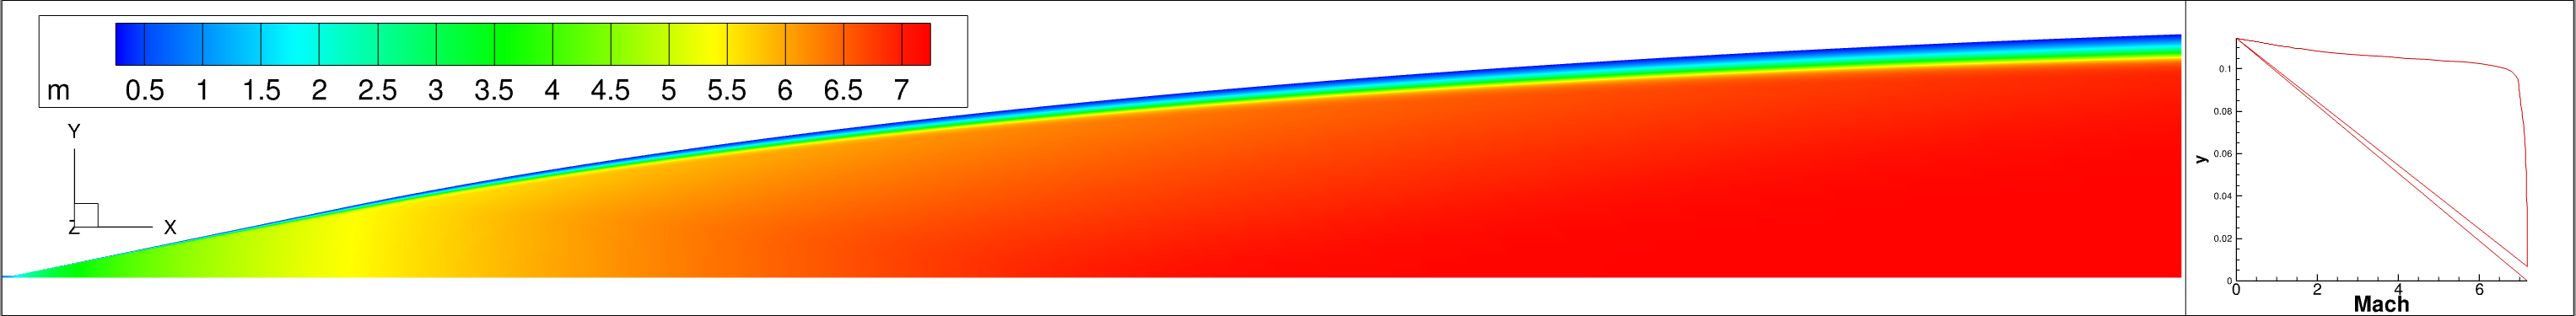
\includegraphics[width=6in]{ace2-cfd}
    \caption{ACE2.0 CFD Mach number plot}
    \label{fig:ace2-cfd}
\end{figure}

\subsection{General Nozzle and Settling Chamber Design}

The resulting contour from above was imported into Solidworks using the analytic equations given in Appendix \ref{appendix:contour}, and the new ACE2.0 nozzle and settling chamber were designed following the above requirements. In order to accommodate the active control, the nozzle and settling chamber were combined into single rigid upper and lower pieces. Similar to ACE, the last 4 inches of the nozzle is a separate flexure piece to enable the variable Mach number capability. The overall length of the nozzle and settling chamber was increased by 19 inches with most of the added length contributed to the settling chamber. 

The settling chamber is 1.7 inches taller and has a few considerable improvements. The flow conditioners are enclosed in a standalone box that allows for easy maintenance and future modifications of screen configurations. The initial configuration provides 3 inches between each aerogrid and screen for adequate turbulence decay. Inlet flow spreaders are added as well to allow uniform mixing of the incoming air before flowing through the aerogrids. 

The ACE design had the relative motion interface between nozzle and settling chamber with a large rubber seal that struggled to properly seal at higher Mach numbers. For ACE2.0, the end of the settling chamber is split into two pieces to allow the rotation of the nozzle blocks. This moves the potential sealing issue upstream of the flow conditioners where minor leaks are much less of a concern. The final ACE2.0 nozzle and settling chamber design compared to ACE is shown in Figure \ref{fig:nozzles}. 

\begin{figure}[ht!]
    \centering
    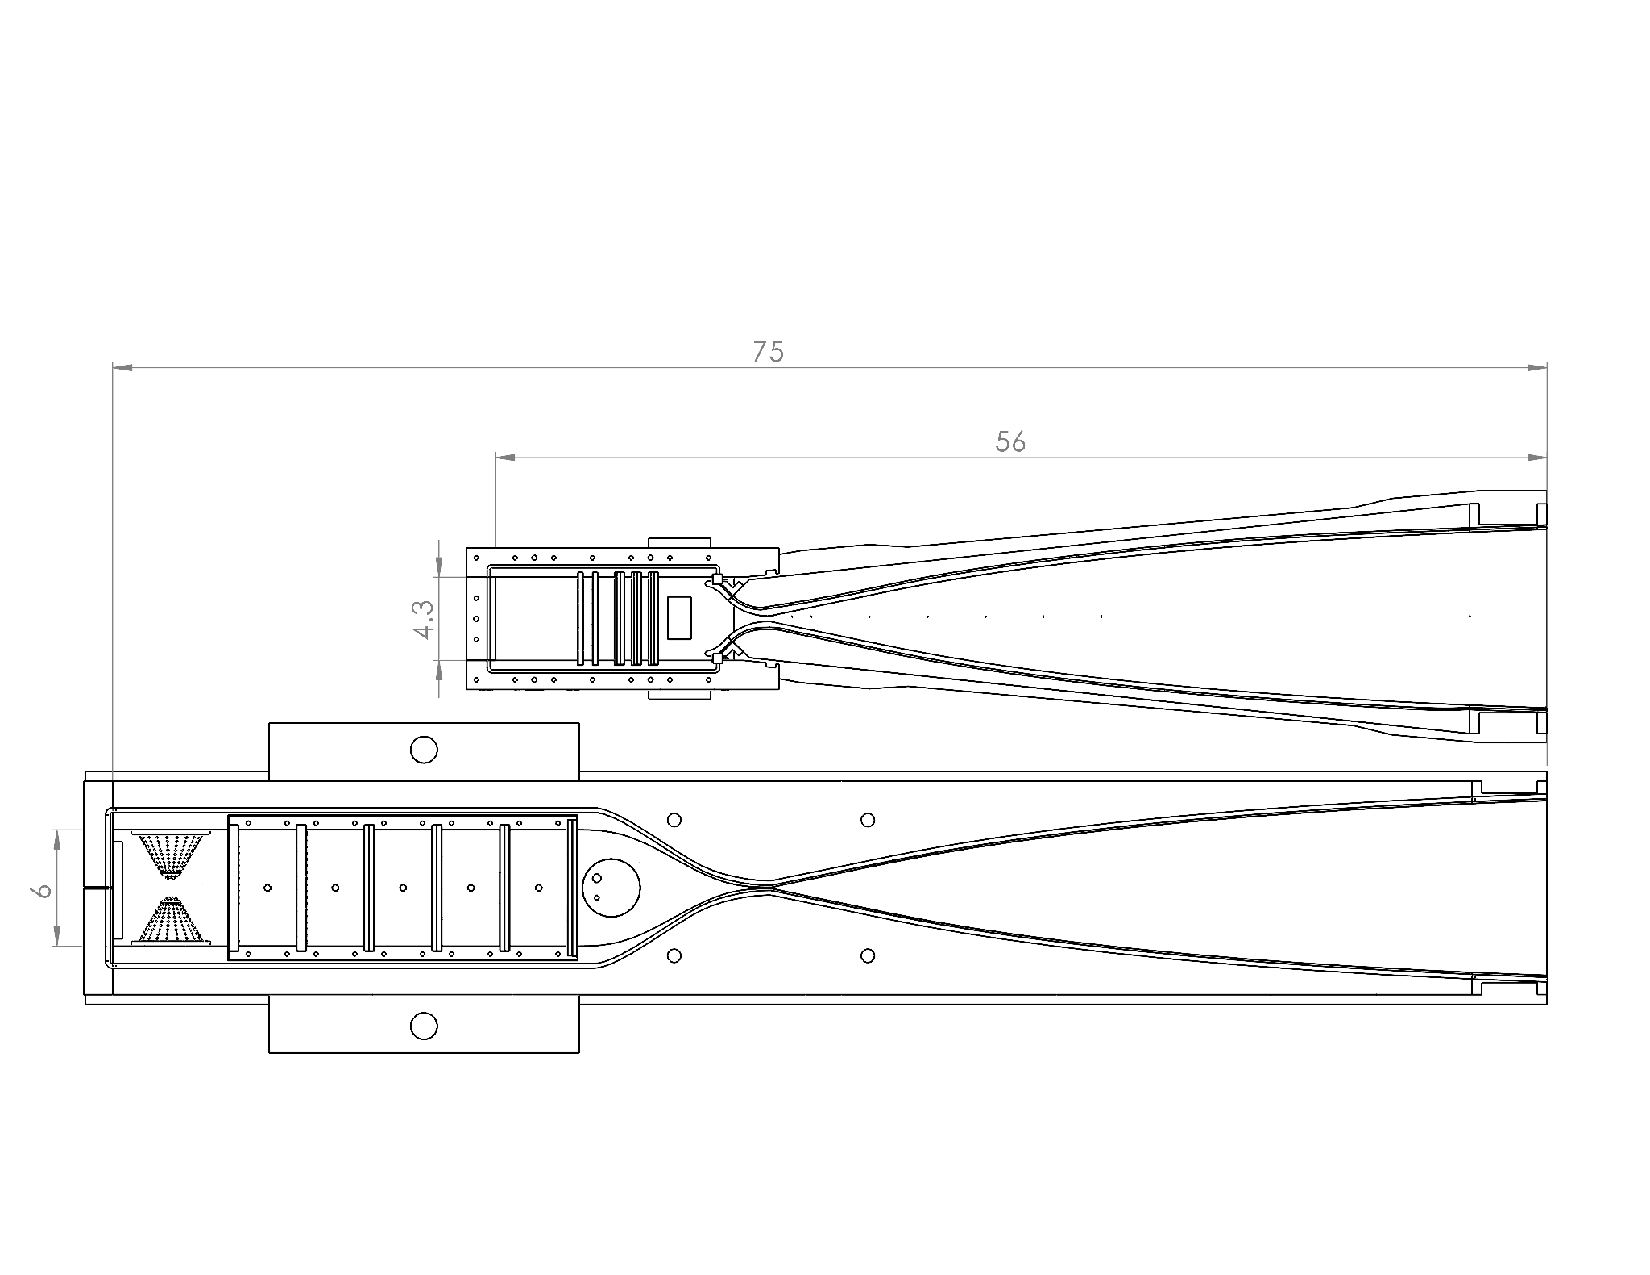
\includegraphics[trim={12 100 40 162},clip,width=6in]{nozzles.pdf}
    \caption{Comparison of ACE (top) and ACE2.0 (bottom) nozzle and settling chamber designs}
    \label{fig:nozzles}
\end{figure}

All of the nozzle and settling chamber parts will be made from 304 stainless steel except for the flexures, which will be made from Condition A 17-4 PH stainless steel for maximum strength while maintaining flexibility.

\subsection{Mechanical Design Iterations}

There were a few distinct iterations throughout the design process of ACE2.0 that are worth mentioning briefly. As mentioned, enabling active control was not the original intent of the ACE redesign, so the initial mechanical design was limited. One major difference to note between all of the past iterations and the final iteration is that the nozzle and settling chamber upper and lower pieces are not single rigid parts in the past iterations. The plan was to have either a bolted or welded interface between the nozzle blocks and the settling chamber piece to save cost in stock material, but it was decided to accept the higher cost of material for maximum strength and rigidity with a single piece.

A preface to the mechanical designs is that the actual load on the settling chamber and nozzle at a maximum pressure of 200 psia is around 90,000 pounds per top and bottom. This is the result of the increased surface area of the settling chamber and subsonic portion of the nozzle, which together is 14 inches wide by 36 inches long.

The first iteration, shown in Figure \ref{fig:i1}, had a system of worm gears and lead screws to simultaneously adjust both nozzle blocks, and it required a jam nut on each lead screw and large wedges on the settling chamber to lock the position during a run. This design was not intended to be active, so it could not dynamically support the loads during a run. This design revealed that active control was not far from reach, so the next iteration began with the intention to enable it.

\begin{figure}[ht!]
    \centering
    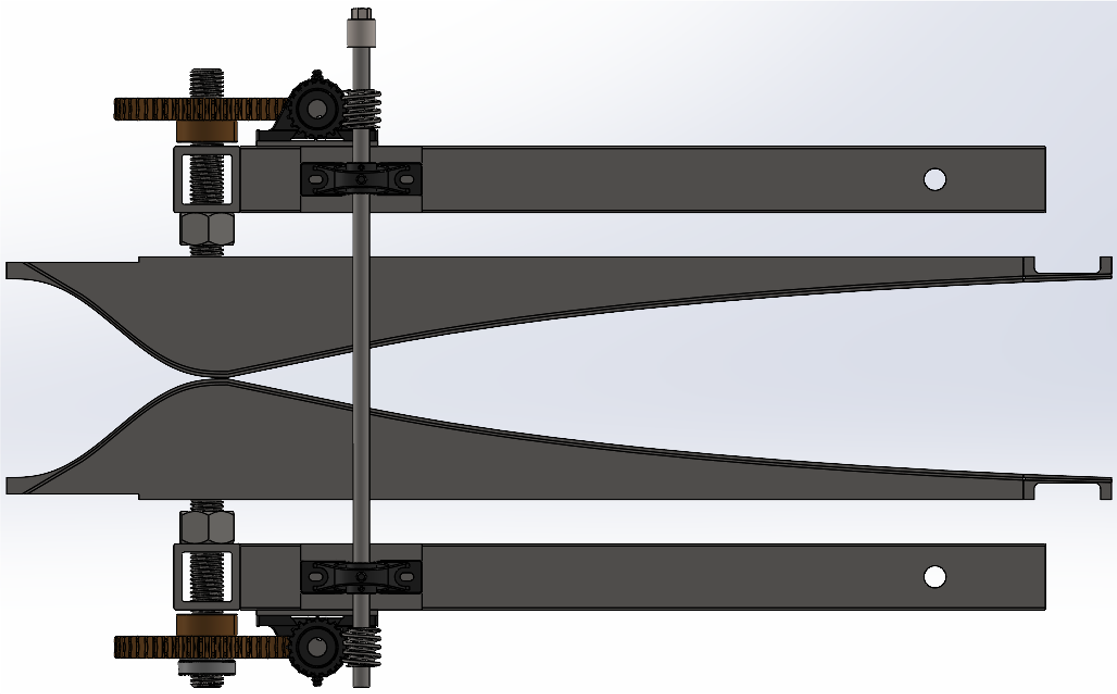
\includegraphics[width=5in]{i1a}
    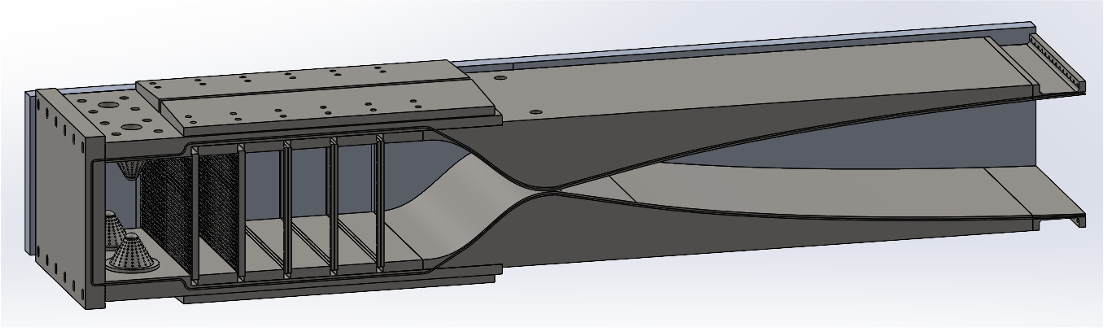
\includegraphics[width=5in]{i1b}
    \caption{Iteration 1 of ACE2.0: Non-active}
    \label{fig:i1}
\end{figure}

The second iteration, shown in Figure \ref{fig:i2}, built off from the idea of the wedges on the settling chamber to fully support against the loads during a run. This design relied on specially contoured oi-impregnated bronze sliding plates that were actuated by a similar system of worm gears and lead screws. The purpose of the contours instead of a simple flat wedge was to (1) provide a constant rate of change for the Mach number given a constant lead screw translation rate input and (2) maintain all points of contact as the nozzle rotated. The primary concern with this design was the expected wear and required actuation force due to friction, which would be around 20,000 pounds assuming a friction coefficient of 0.2 between the stainless steel and oil-impregnated bronze. This design also had the introduction of the disc spring stacks at the settling chamber end to hold the nozzles apart at the set position while not under load. 

\begin{figure}[ht!]
    \centering
    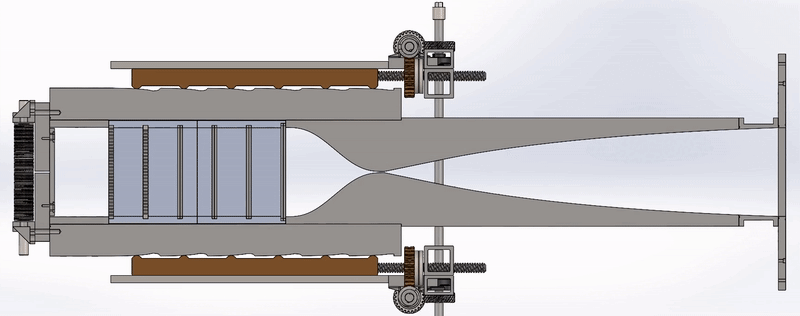
\includegraphics[width=6in]{i2}
    \caption{Iteration 2 of ACE2.0: Sliding Wedge}
    \label{fig:i2}
\end{figure}

The third iteration, shown in Figure \ref{fig:i3}, improved upon the previous approach by introducing rollers and bearings to eliminate the friction and linear actuators for simpler and more robust control. This design was abandoned for two primary reasons: (1) a realization that the reverse load while under full vacuum was unsupported and (2) feedback from machinists about concerns of wear in bearings and difficulty in machining the roller plate. The load under full vacuum across the entire nozzle and settling chamber is around 16,000 pounds, which requires substantial support to maintain the set Mach number when initiating a run and to minimize excess loads on the flexure.

\begin{figure}[ht!]
    \centering
    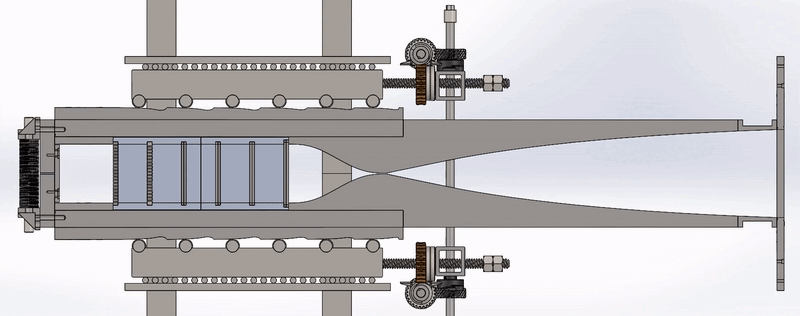
\includegraphics[width=6in]{i3}
    \caption{Iteration 3 of ACE2.0: Rollers and Actuators}
    \label{fig:i3}
\end{figure}

The fourth and final iteration turned to a complete different approach of using 20-ton ball screw linear actuators to fully support both the maximum pressure and full vacuum loads. This final iteration is the most simple mechanically while also providing the most versatility in controlling the Mach number.

\subsection{20-Ton Linear Actuators Design}

The final design of ACE2.0 utilizes two 20-ton ball screw linear actuators on both the upper and lower nozzle blocks to actively control the Mach number by varying the throat height. The final design of the nozzle and settling chamber with the actuators can be seen in Figure \ref{fig:cad-nozzle-actuators}. 

\begin{figure}[ht!]
    \centering
    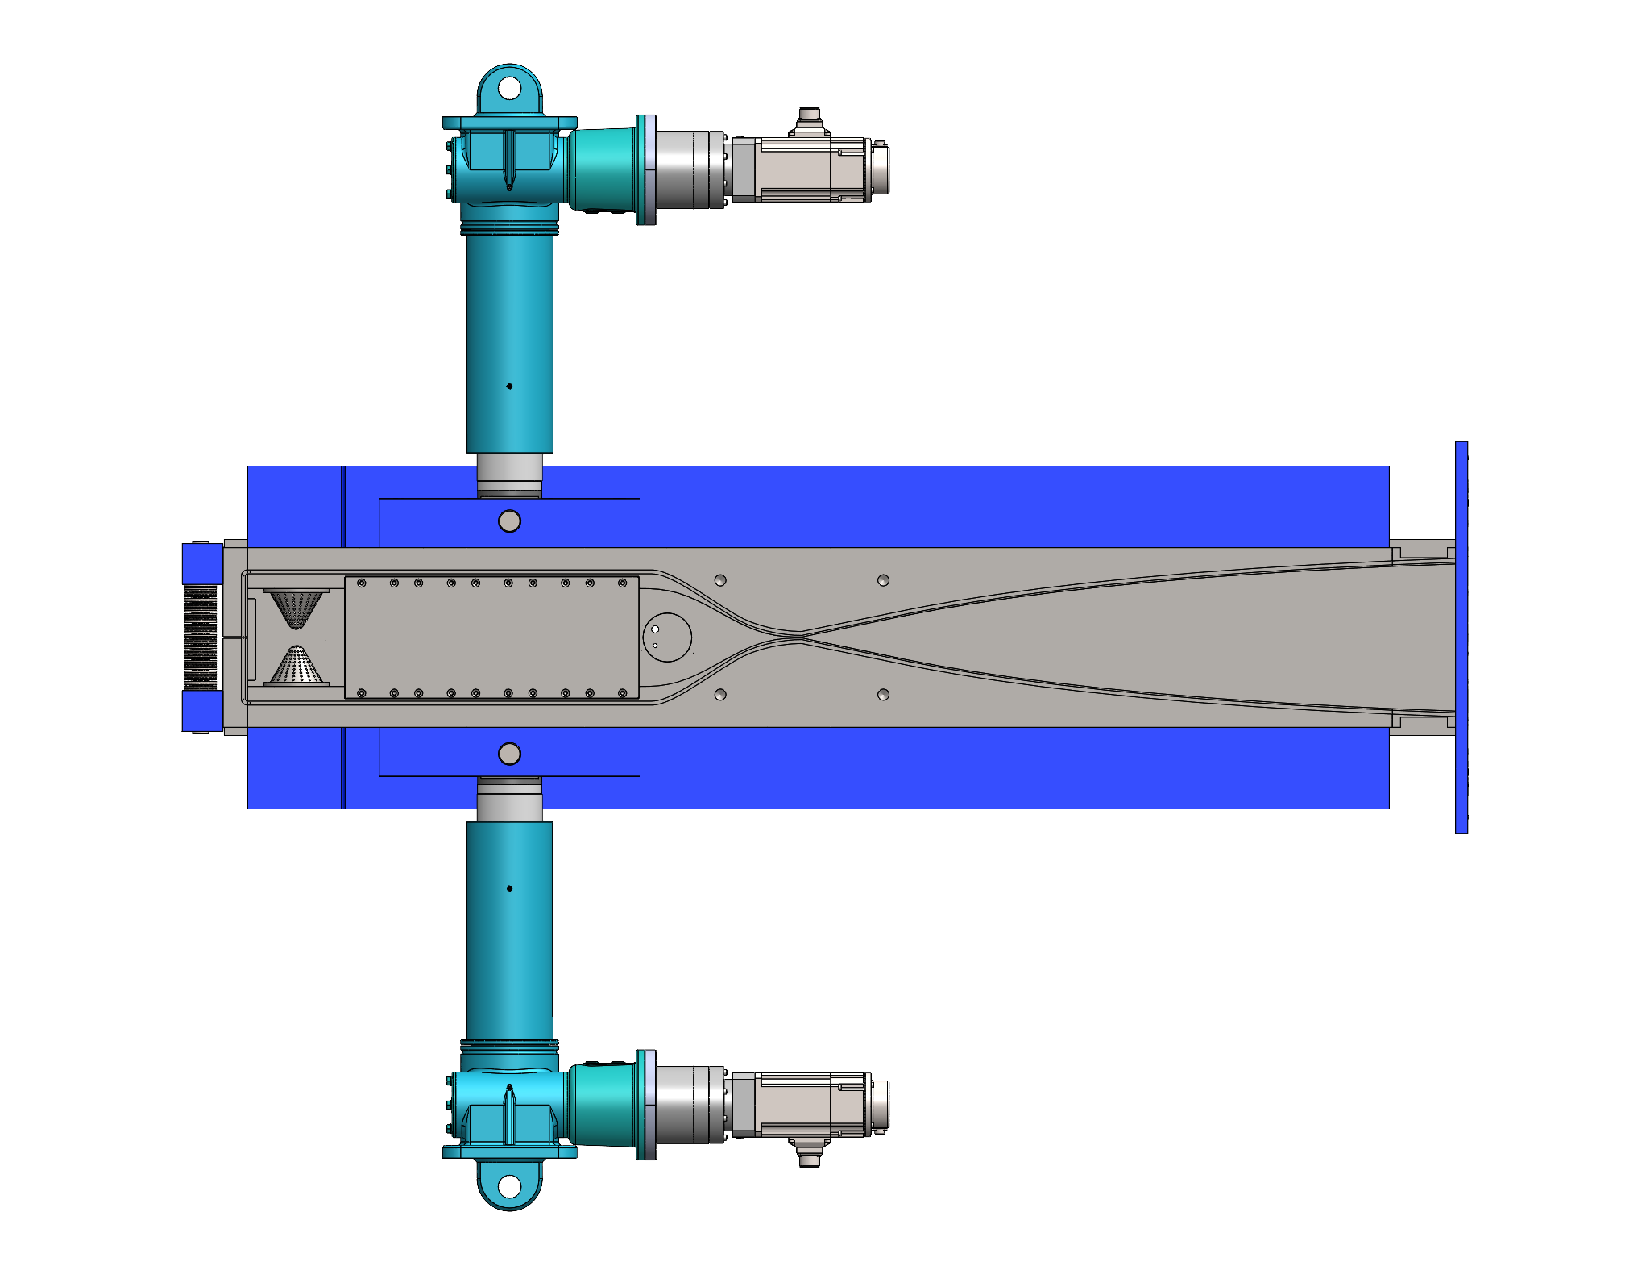
\includegraphics[trim={80 30 80 30},clip,width=5in]{cad-nozzle-actuators.pdf}
    \caption{ACE2.0 final nozzle and settling chamber with actuators.}
    \label{fig:cad-nozzle-actuators}
\end{figure}

\subsubsection{Nozzle and Settling Chamber Design}

Using linear actuators does present the challenges of introducing stress concentrations at the attachment location and not providing support along the length of the nozzle and settling chamber. These were overcome by making the mating clevis on the settling chamber a 16 inch bar to distribute the load and adding a 5 inch by 2.5 inch beam along the length of the nozzle and settling chamber to provide rigidity, as seen in Figure \ref{fig:cad-nozzle-actuators}.

The sidewalls are 1.5 inches thick and made from 304 stainless steel. They are handled and suspended from the frame by two brackets each, and a series of custom bar clamps will provide the support against the load under pressure. One sidewall has all of the ports and sensors, which allows the other to be the main access for maintenance. \textcolor{red}{Go into details of ports with figures?}

The flow conditioner box is made from four 0.75 inch thick 304 stainless steel plates. This assembly floats between the nozzles and is secured by the sidewalls in a slot. The overall height doubles as a safety limit so the nozzles will hit each side of the box before hitting each other. Housed inside the box is two aerogrids and four screens in the current configuration, but any configuration can easily be designed and swapped in the future. \textcolor{red}{Figure? And go into further detail on aerogrids and screens?}

\subsubsection{Frame Design}

The frame was designed around the linear actuators to best support the extreme loads. In order to maximize strength, a single piece brace was designed to symmetrically bear the loads from the actuators. The rest of the frame was designed between the brace and the nozzle-test-section flange to support the sidewalls. The entire frame will be made from 3 inch thick 4140 alloy steel plates and bars, and it all bolts together instead of welding. All exposed faces will be powder coated in order avoid rust and wear over time. 

The frame will have four 5000-pound capacity steel swivel casters for easy maneuvering when aligning for installation. Once in position, the weight of the assembly will be transferred to rigid feet on threaded rods. All of these details can be seen in Figure \ref{fig:cad-frame}.

\begin{figure}[ht!]
    \centering
    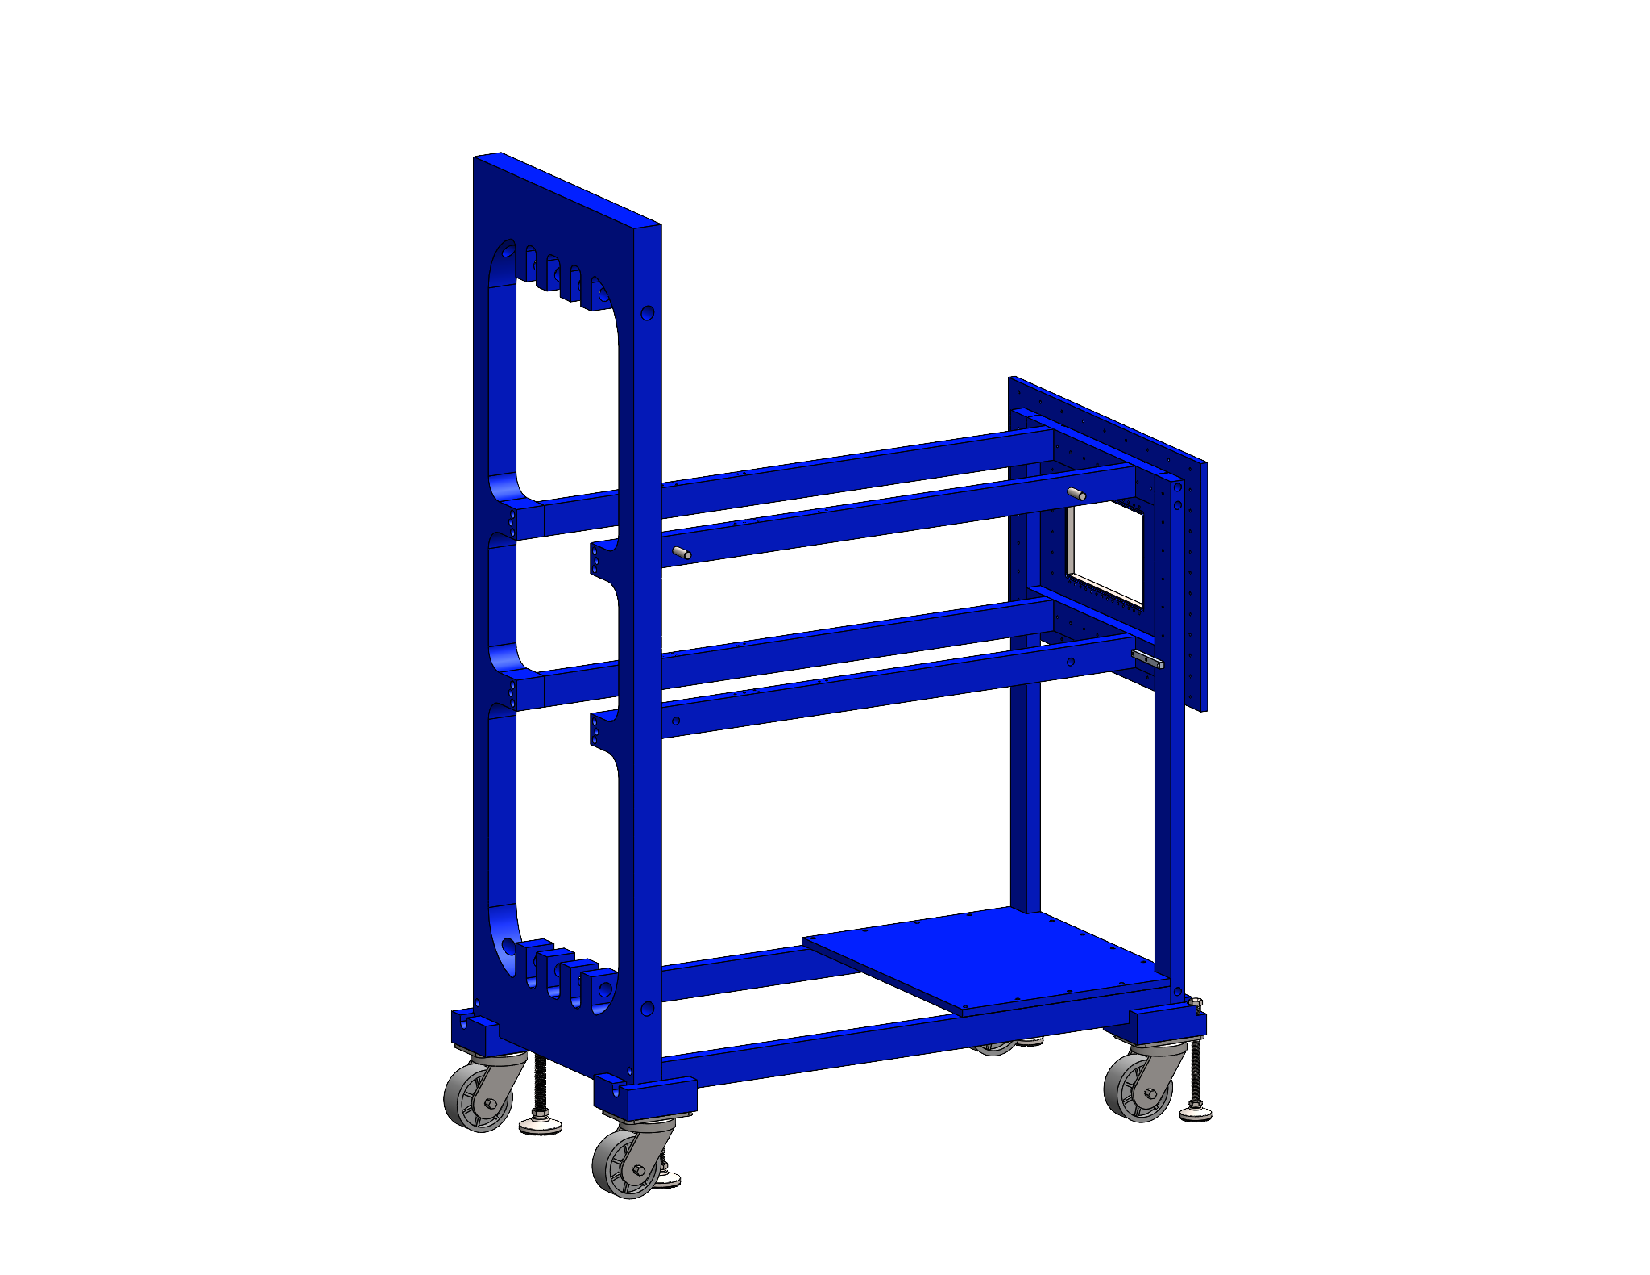
\includegraphics[trim={160 30 160 70},clip,width=6in]{cad-frame.pdf}
    \caption{CAD of frame}
    \label{fig:cad-frame}
\end{figure}

\subsubsection{Actuation System Design}

The actuation system for ACE2.0 is comprised of many components that enable the active  feedback-back control of the Mach number. Only a high level overview will be provided here for sake of brevity, but a full detailed description of the entire system will be provided in Appendix \ref{appendix:actuation}. 

The linear actuators are each rated for 40,000 pounds with a minimum FOS of 7. They have a double clevis design to rotate freely and have a custom motor mount for the selected gear box and servo motor, as shown in Figure \ref{fig:actuators}. The actuators are comprised of a 24:1 worm gear reducer that turns a ball nut to drive a 0.5 inch lead ball screw. The ball nut has a long service life that will allow over 400,000 full throat deflections before maintenance is required. Another 20:1 gear box will be mounted to each actuator for an overall travel of approximately 0.001 inch per servo motor turn.

\begin{figure}[ht]
    \centering
    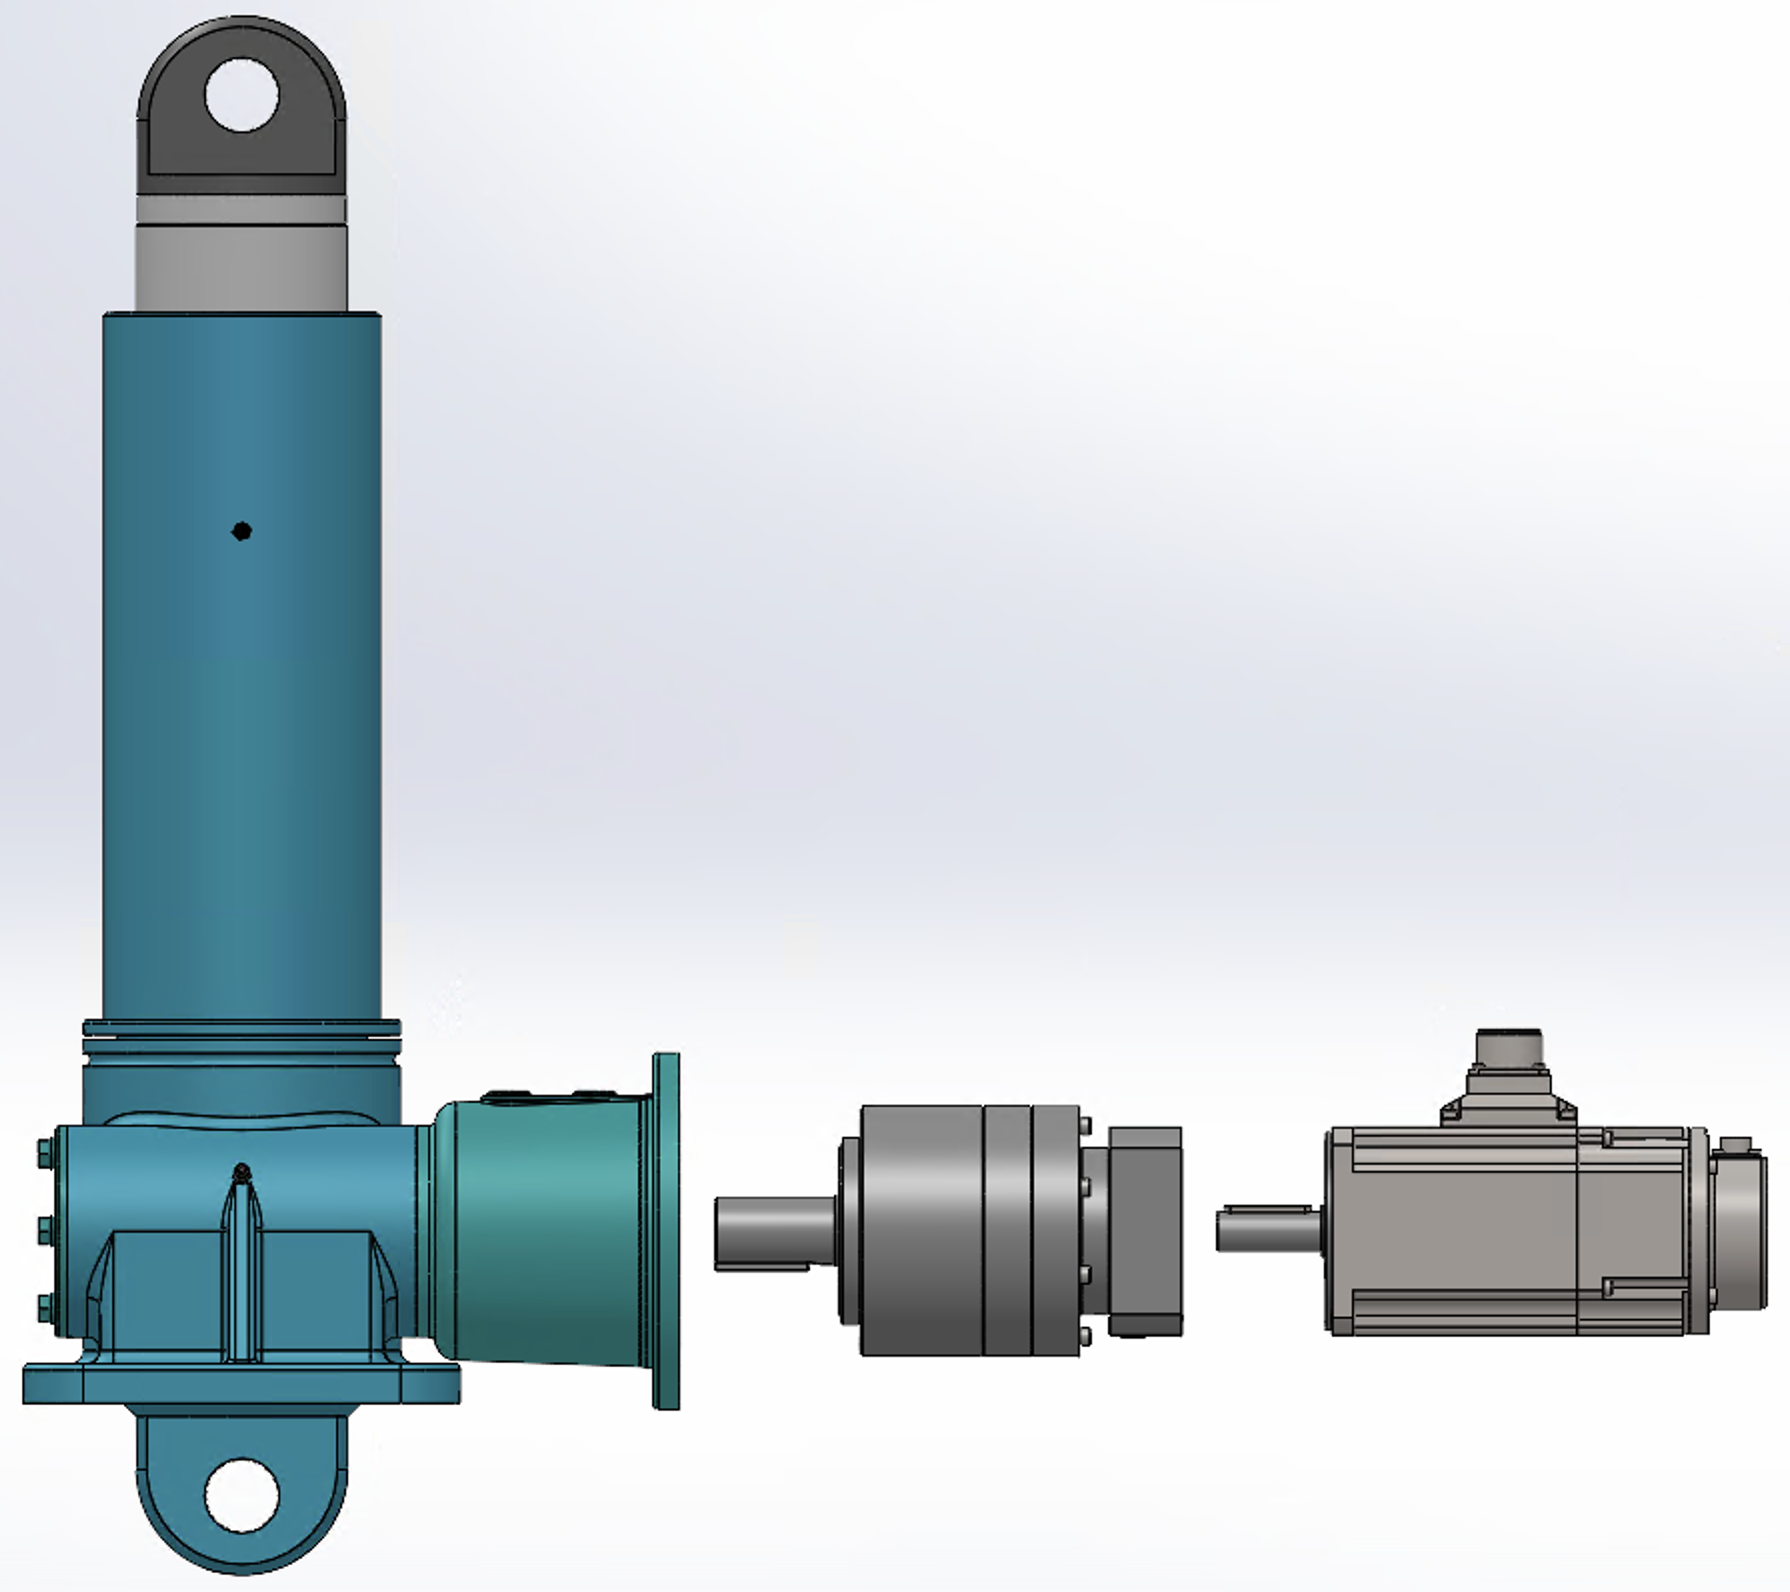
\includegraphics[width=5in]{actuators}
    \caption{CAD model of 20-ton linear actuator, 20:1 gear box, and servo motor.}
    \label{fig:actuators}
\end{figure}

The required input torque for the actuators at maximum load with the additional gearbox is 28 inch-pounds. The rated continuous torque and the momentary peak torque of the selected servo motor are 28 and 84 inch-pounds, respectively, and the rated continuous speed and the momentary peak speed are 3000 and 5000 revolutions per minute, respectively. The change in throat height from Mach 5 to 8 for each half of the nozzle is around 0.157 inches, so a full Mach sweep at maximum pressure can be achieved in around 3 seconds within the continuous operation range of the servo motor. The servo motors have a power-off brake hold a set Mach number and to prevent motion and any potential damage in a power outage.

In order to minimize the backlash in the actuators, two inverted stacks of Belleville disc springs were added to the end of the settling chamber as shown in Figure \ref{fig:springs}. With a nominally linear relationship between force and compression, a stack height of 8 inches and minimum compression of 0.875 inches was chosen to produce a combined minimum force of 3000 pounds to always lift the upper nozzle block and keep the actuators in compression.

\begin{figure}[ht!]
    \centering
    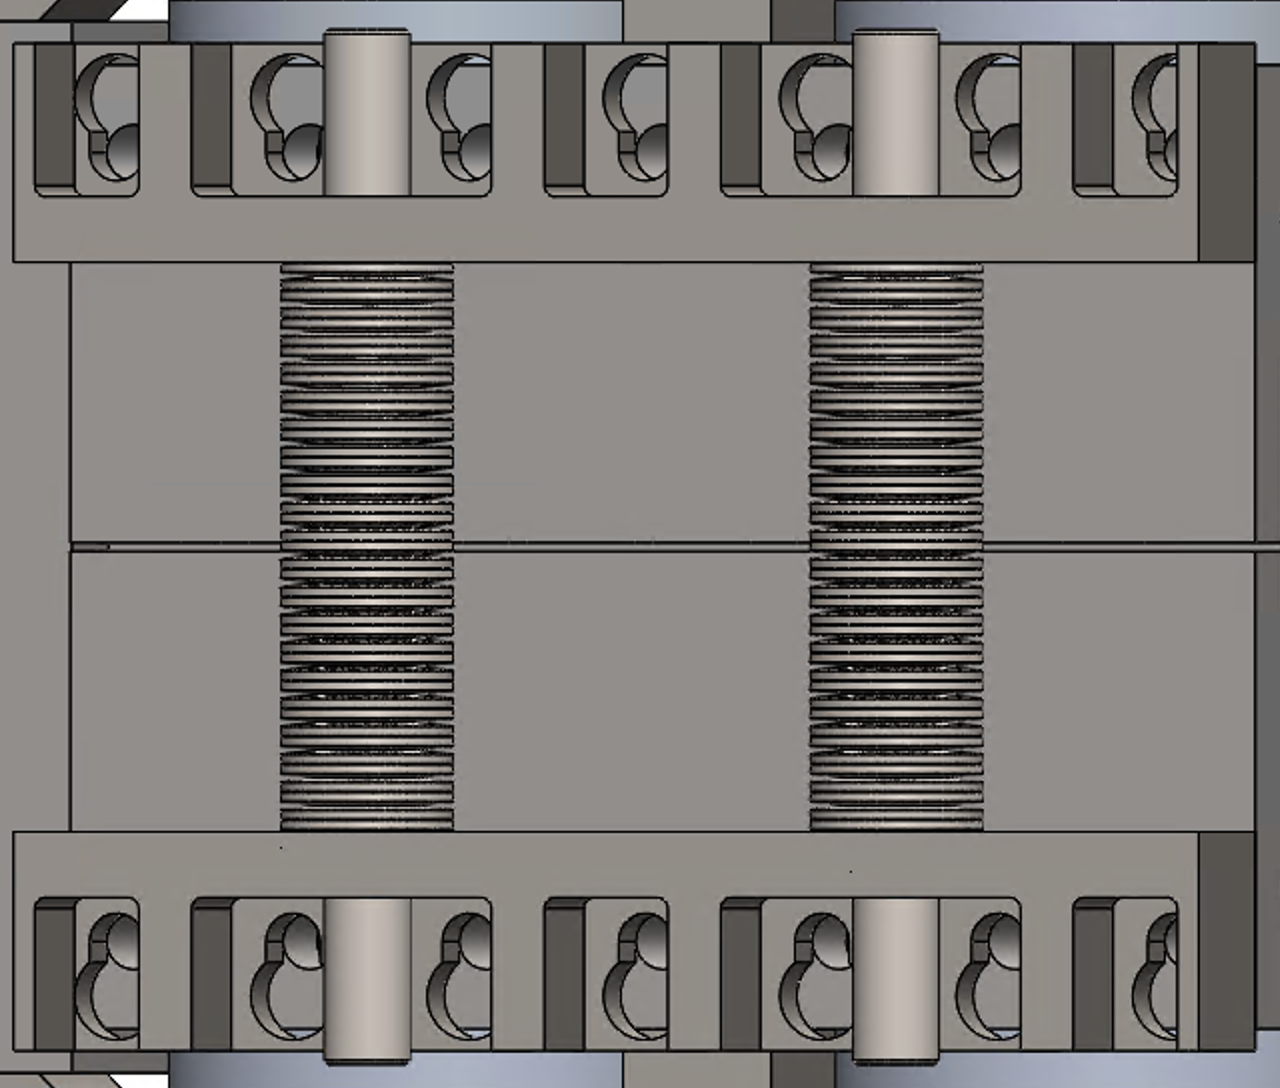
\includegraphics[width=5in]{springs}
    \caption{Inverted disc springs stacks at the end of the settling chamber.}
    \label{fig:springs}
\end{figure}

The four servo motors are each driven by individual servo drives powered by 240 VAC 3-phase. These four drives and servo motors are controlled synchronously by a programmable logic controller (PLC) through EtherCAT, the fastest industrial Ethernet communication protocol. The PLC logic programs are written its associated software, Sysmac Studio. This software is a graphical ladder logic environment designed to integrate many automation devices across EtherCAT.

The specific program to control the Mach number will be created in future work. This program will initially be designed with four control objectives: (1) precise set Mach number, (2) Mach number sweep with specified start, stop, and time, (3) Mach number schedule, and (4) feedback-control for Mach number. The completed Mach number control program will be provided in Appendix \ref{appendix:actuation}. Additionally, three analog modules were added to the PLC to input the static pressure, stagnation pressure, and temperature measured by the corresponding sensors to enable feedback-control. 

Additional components of the system include two safety limit switches for each actuator, an external encoder for each actuator for additional physical feedback, various power supplies and relays, an emergency stop button, and a 7" human machine interface (HMI) for a simple control interface that can be updated and expanded for any desired controls.

\subsubsection{Final Overall Design}

The final design with all modeled components is shown in Figure \ref{fig:cad-full}. The entire design will integrate with the existing ACE test section and other infrastructure. The overall length from the nozzle-test-section flange to the inlet of the 4-way manifold is 94 inches, shown in Figure \ref{fig:cad-side}, which is only around 12 inches longer than ACE.

\begin{figure}[ht!]
    \centering
    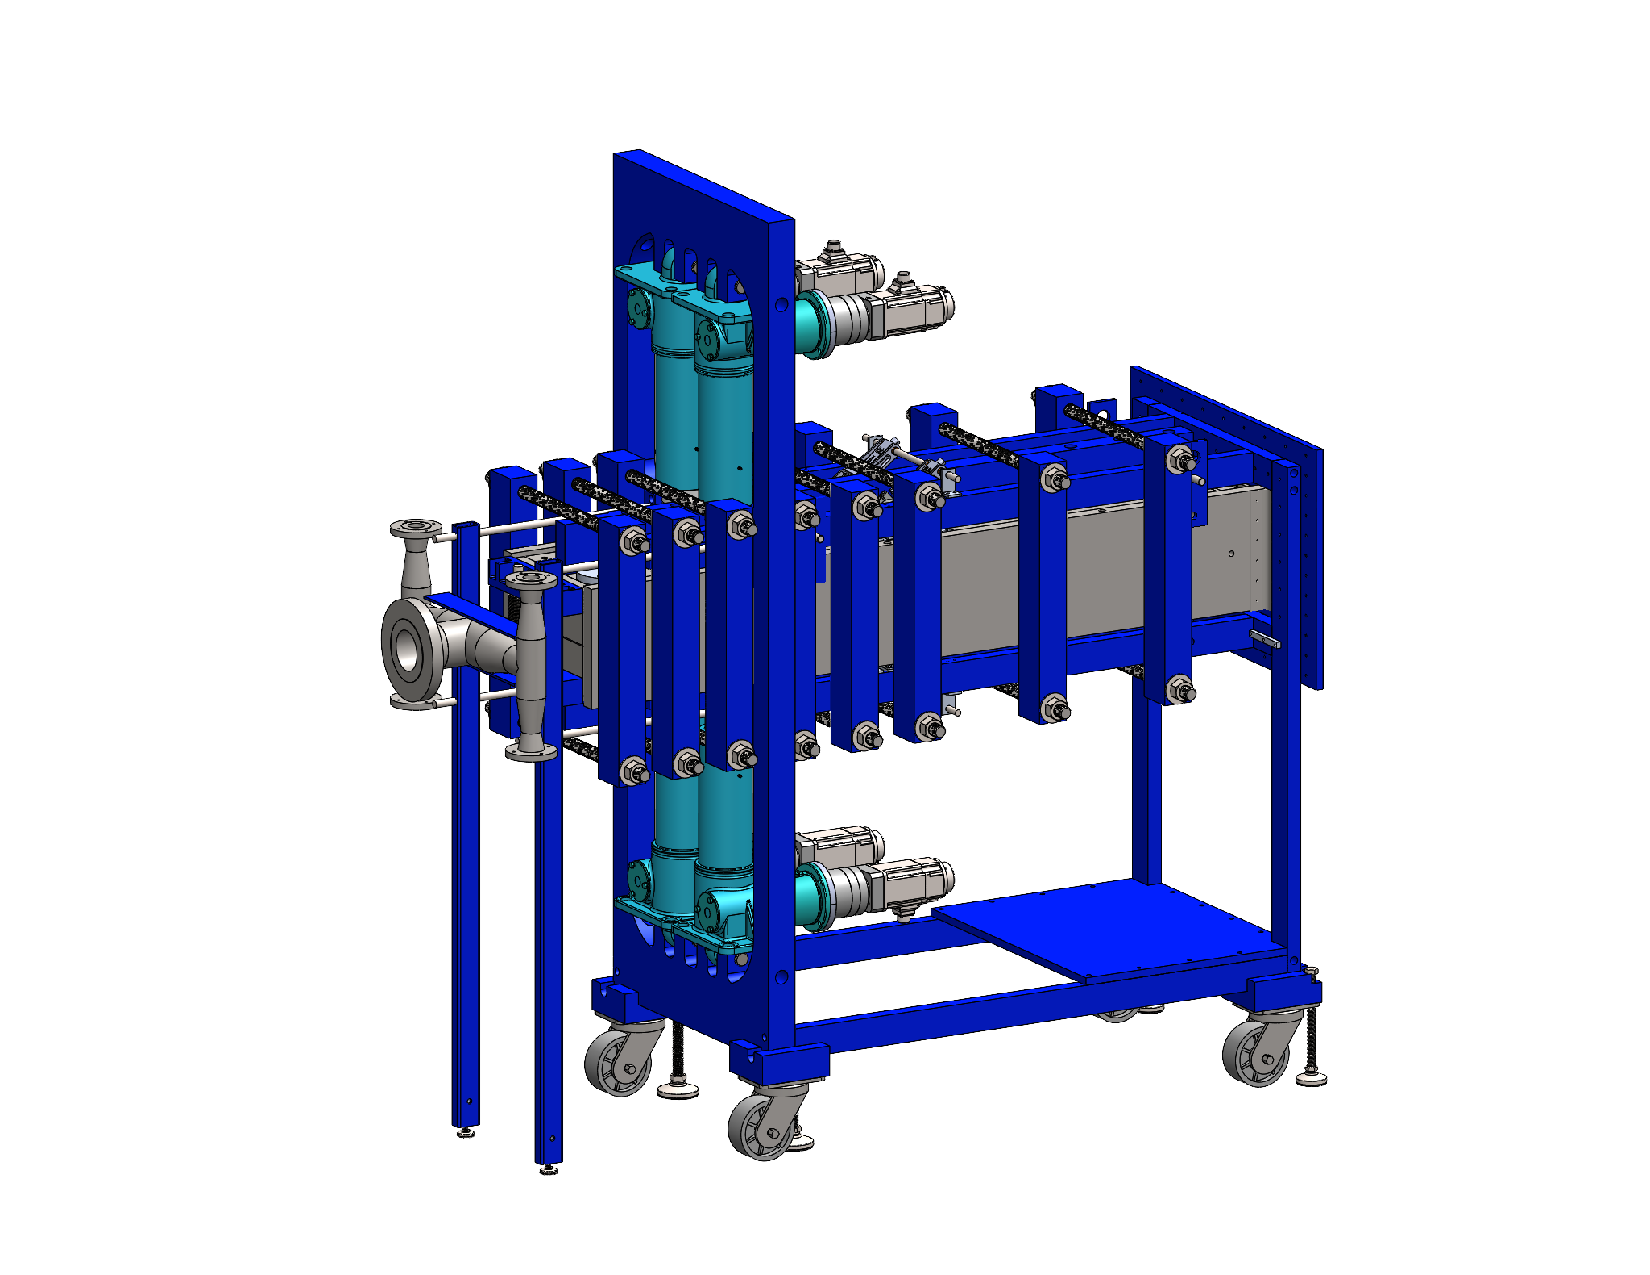
\includegraphics[trim={180 30 135 70},clip,width=6in]{cad-full.pdf}
    \caption{Full CAD model of ACE2.0 in Solidworks}
    \label{fig:cad-full}
\end{figure}

\begin{figure}[ht!]
    \centering
    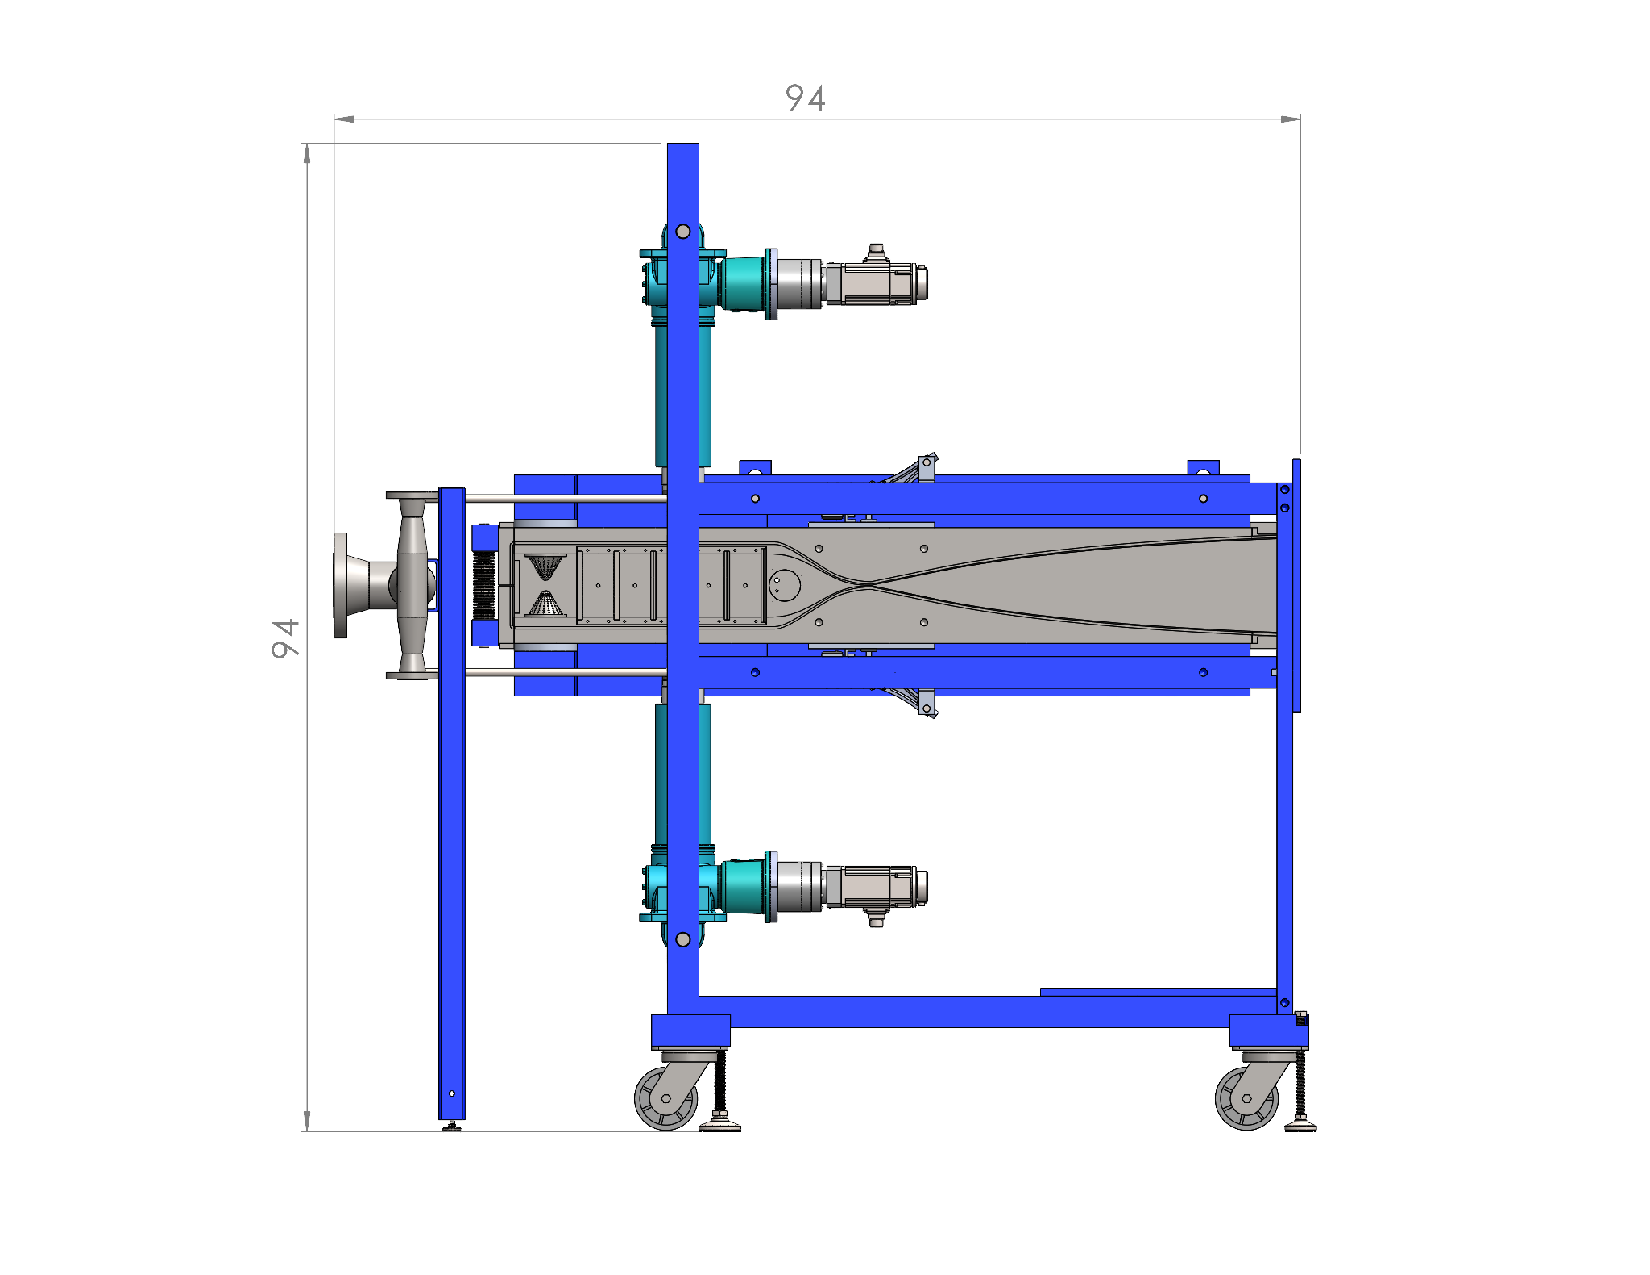
\includegraphics[trim={130 50 150 30},clip,width=6in]{cad-side.pdf}
    \caption{Side view of ACE2.0 in Solidworks}
    \label{fig:cad-side}
\end{figure}

\subsubsection{FEA}

The structural integrity of the final design was simulated using finite element analysis (FEA) in Solidworks. There were four primary simulations conducted: (1) lower nozzle and settling chamber at 200 psia with gravity, (2) upper nozzle and settling chamber at full vacuum with gravity, (3) sidewall with clamps at 200 psia, (4) and flexure fatigue at maximum deflection.

From all of these simulations, the minimum FOS achieved was 1.8. \textcolor{red}{Flexure fatigue results...} 

\textcolor{red}{What figures to show? Show displacement plots? Can show setup with pressure and fixtures. Resulting stress plots are not great to show.}

\section{Fabrication Plans}

\textcolor{red}{How much to detail? Pictures of stock? What parts to show final machined?}

All of the ACE2.0 parts are finished machining besides the nozzles, sidewalls, and brace. The fabrication is following the schedule shown in Figure \ref{fig:schedule}, which shows the completed tasks in gray, the current tasks in green, orange, or red depending on status, and future tasks in white. The frame pieces were machined at the Texas A\&M Fischer Engineering Design Center (FEDC) to utilize their water jet to cut the brace. An image of the brace after being cut out on the water jet is shown in Figure \ref{fig:fab-brace-jet}. The frame parts were originally planned to be water jet from the brace stock as well to save material cost and reduce excess as shown in Figure \ref{fig:cad-water-jet}. It was later discovered that the cost of time and tooling on the water jet to cut all pieces from the 3 inch 4140 alloy steel is about the same as the cost of ordering 60 feet of bar stock. The decision to order the bar stock was made to allow the water jet to be used for other parts while the bar stock shipped and delivered. The pallet of finished frame parts is shown in Figure \ref{fig:fab-frame-parts}.

\begin{figure}[ht!]
    \centering
    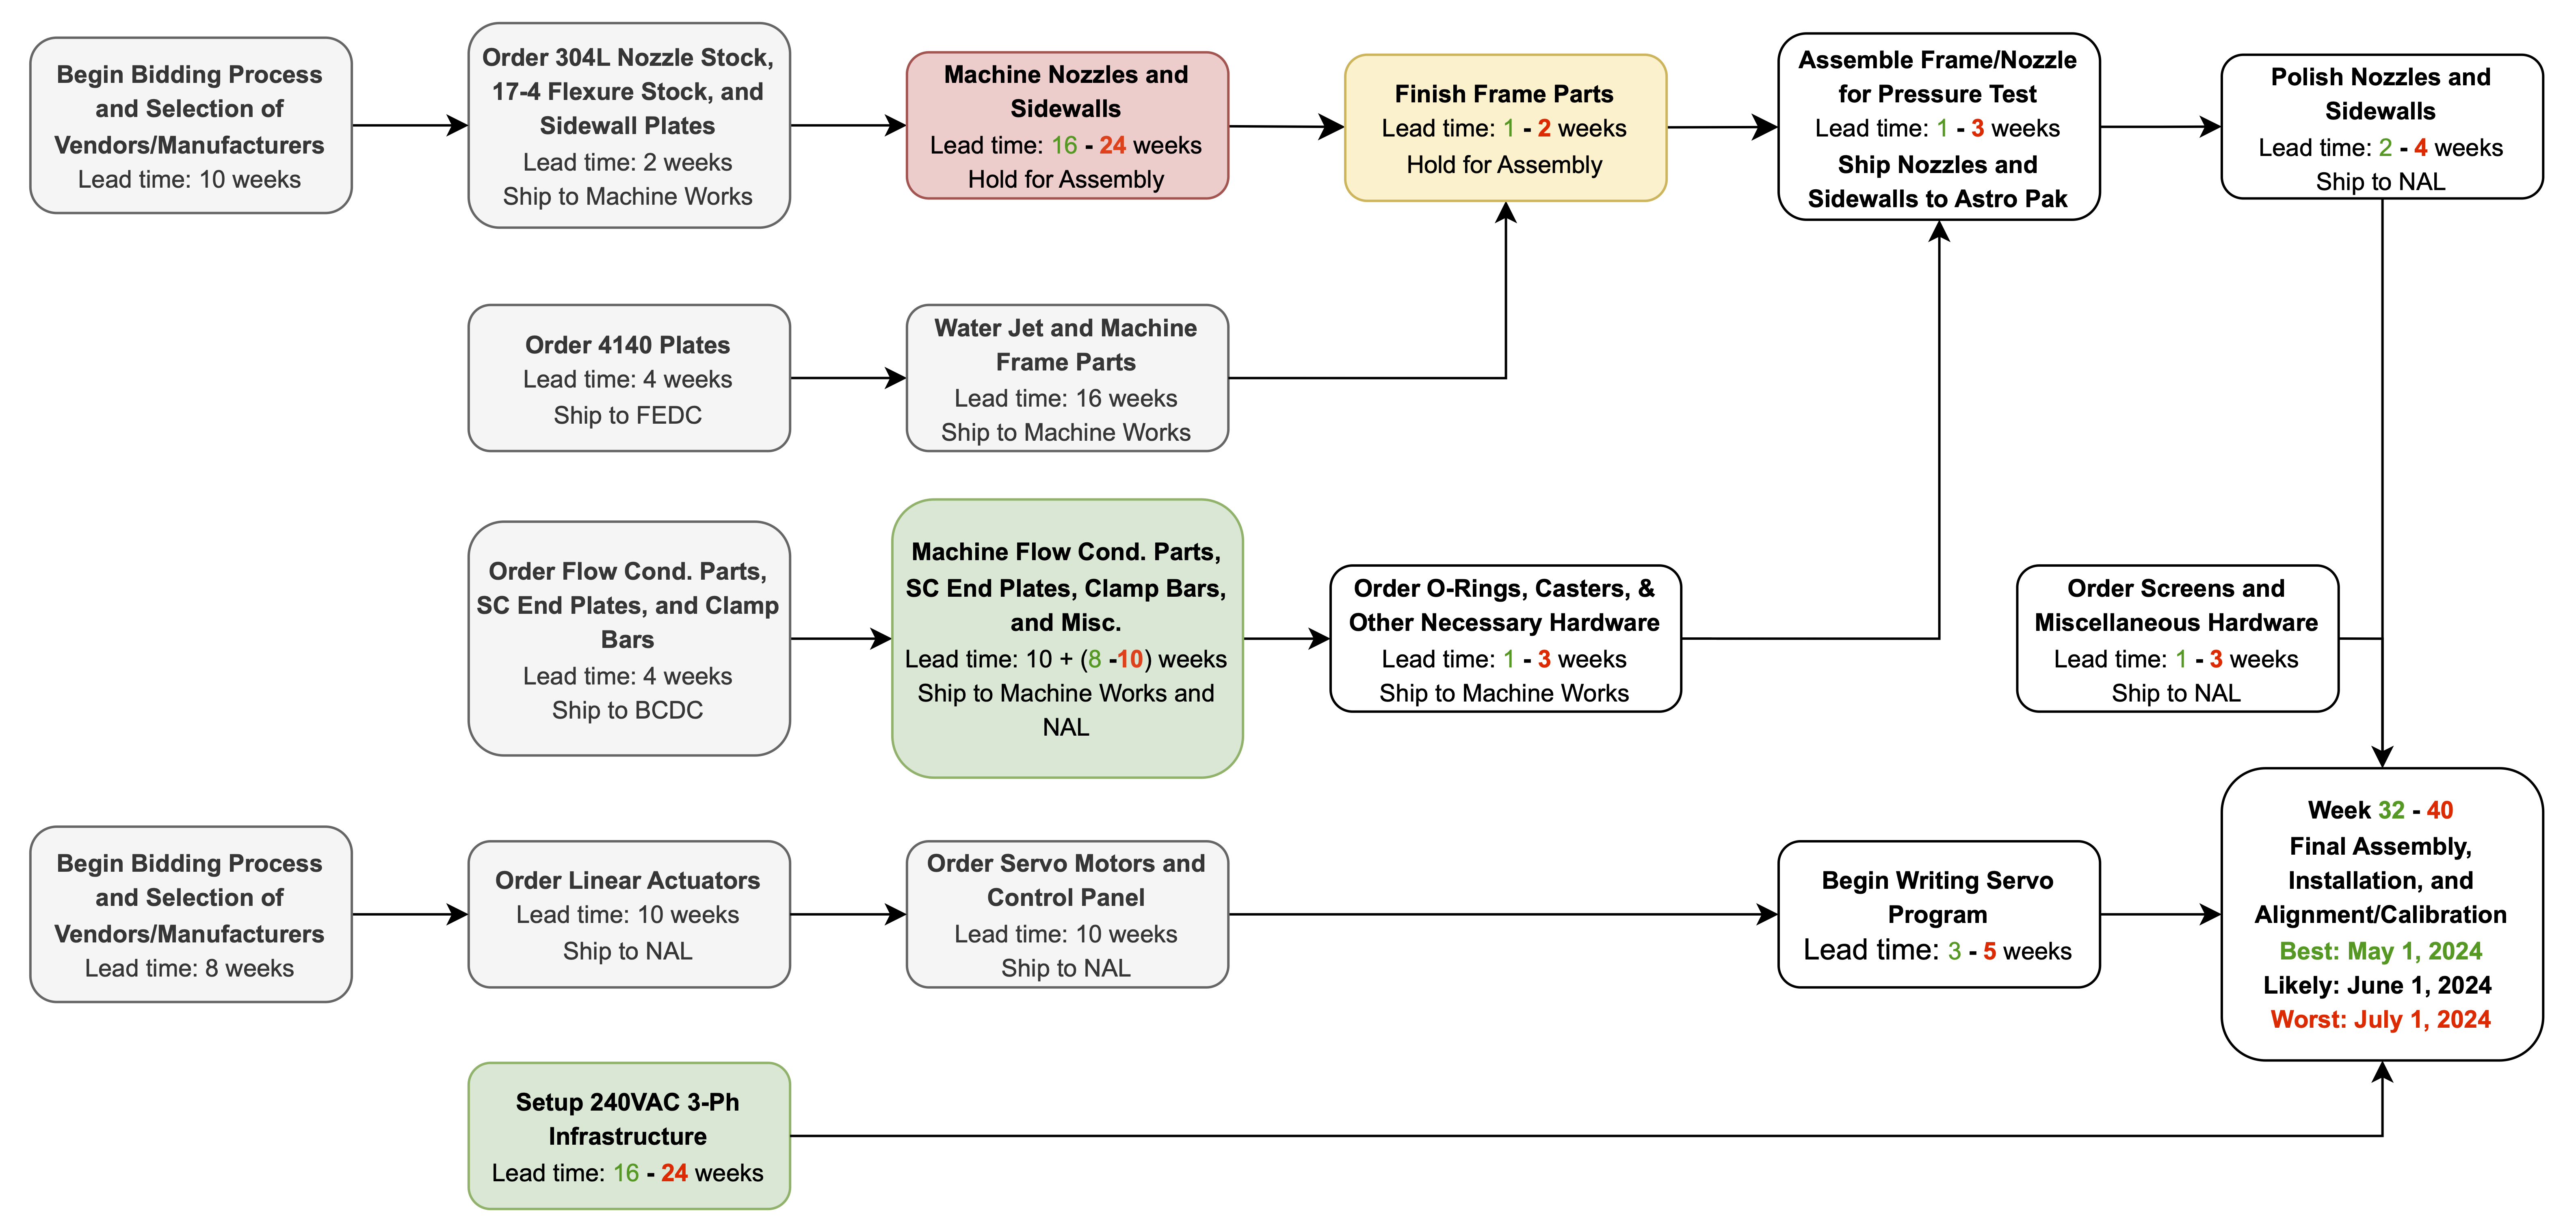
\includegraphics[width=6in]{schedule}
    \caption{Manufacturing schedule beginning from September 25, 2023.}
    \label{fig:schedule}
\end{figure}

\begin{figure}[ht!]
    \centering
    \includegraphics[width=5in]{fab-brace-jet}
    \caption{Rough cut brace on water jet.}
    \label{fig:fab-brace-jet}
\end{figure}

\begin{figure}[ht!]
    \centering
    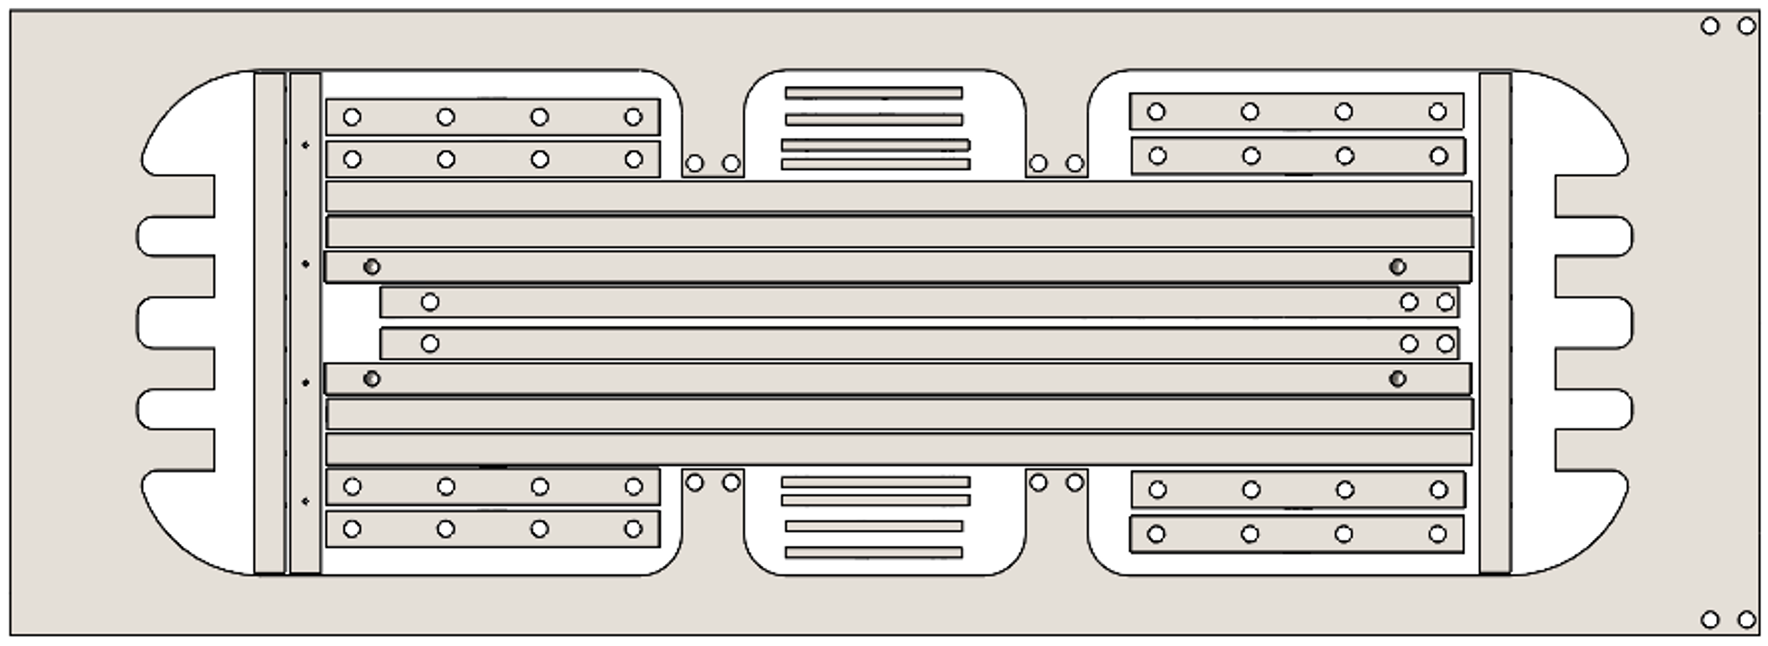
\includegraphics[width=5in]{cad-water-jet}
    \caption{Planned water jet layout for frame parts.}
    \label{fig:cad-water-jet}
\end{figure}

\begin{figure}[ht!]
    \centering
    \includegraphics[width=5in]{fab-frame-parts}
    \caption{Pallet of finished frame parts from FEDC.}
    \label{fig:fab-frame-parts}
\end{figure}

The nozzles and sidewalls are currently being machined at Machine Works Inc. in Bryan, TX. The nozzles were first saw cut to a rough profile to minimize the amount of time on the CNC mill, as shown in Figure \ref{fig:fab-nozzle-saw}. They are currently being machined to a rough contour, and then the back of each will be machined flat prior to finishing the contour. For the final passes, the nozzle blocks and flexures will be bolted together to ensure there is no step between the two pieces. Machine Works will also finish the brace for the frame by drilling and tapping holes.

\begin{figure}[ht!]
    \centering
    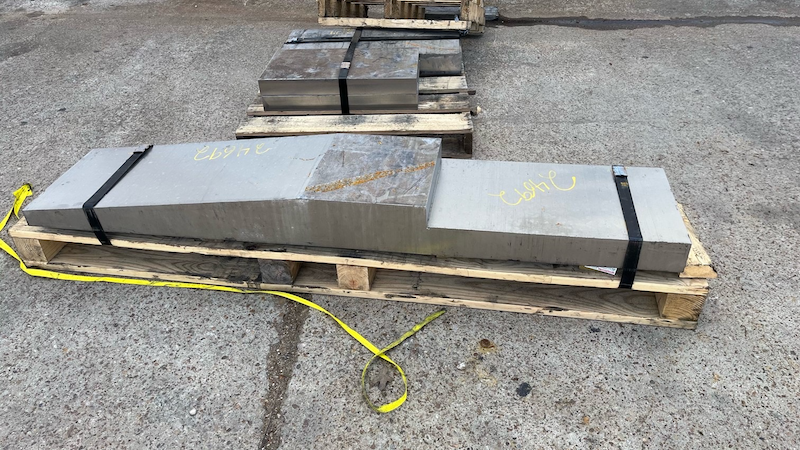
\includegraphics[width=5in]{fab-nozzle-saw}
    \caption{Nozzle block saw cut to rough profile.}
    \label{fig:fab-nozzle-saw}
\end{figure}

The rest of the parts were machined at the Texas A\&M Bush Combat Development Complex (BCDC). All of these parts are finished, but only the parts necessary for the pressure test have been picked up. BCDC will be the primary machine shop for any future fabrication throughout this work.

\subsection{Pressure Test}

The hydro-pressure test will be performed at Machine Works prior to sending the nozzles and sidewalls to be polished. The base tunnel will be assembled with steel bars to simulate the actuators. The tunnel will be filled with water and pressurized to 200 psia for one hour, and the pressure will be monitored throughout. The primary goal of the pressure test is to ensure structural integrity at maximum pressure, but any major leaks will be addressed.

\subsection{Polishing}

Following the completion of the pressure test, the nozzles and sidewalls will be shipped to Astro Pak for polishing. All interior surfaces will be mechanically polished to a 1 Ra finish, and electropolishing will be used if necessary. In order to safely ship these pieces, the nozzle blocks will be assembled as shown in Figure \ref{fig:polish-assembly} and custom wooden crates will be built.

\begin{figure}[ht!]
    \centering
    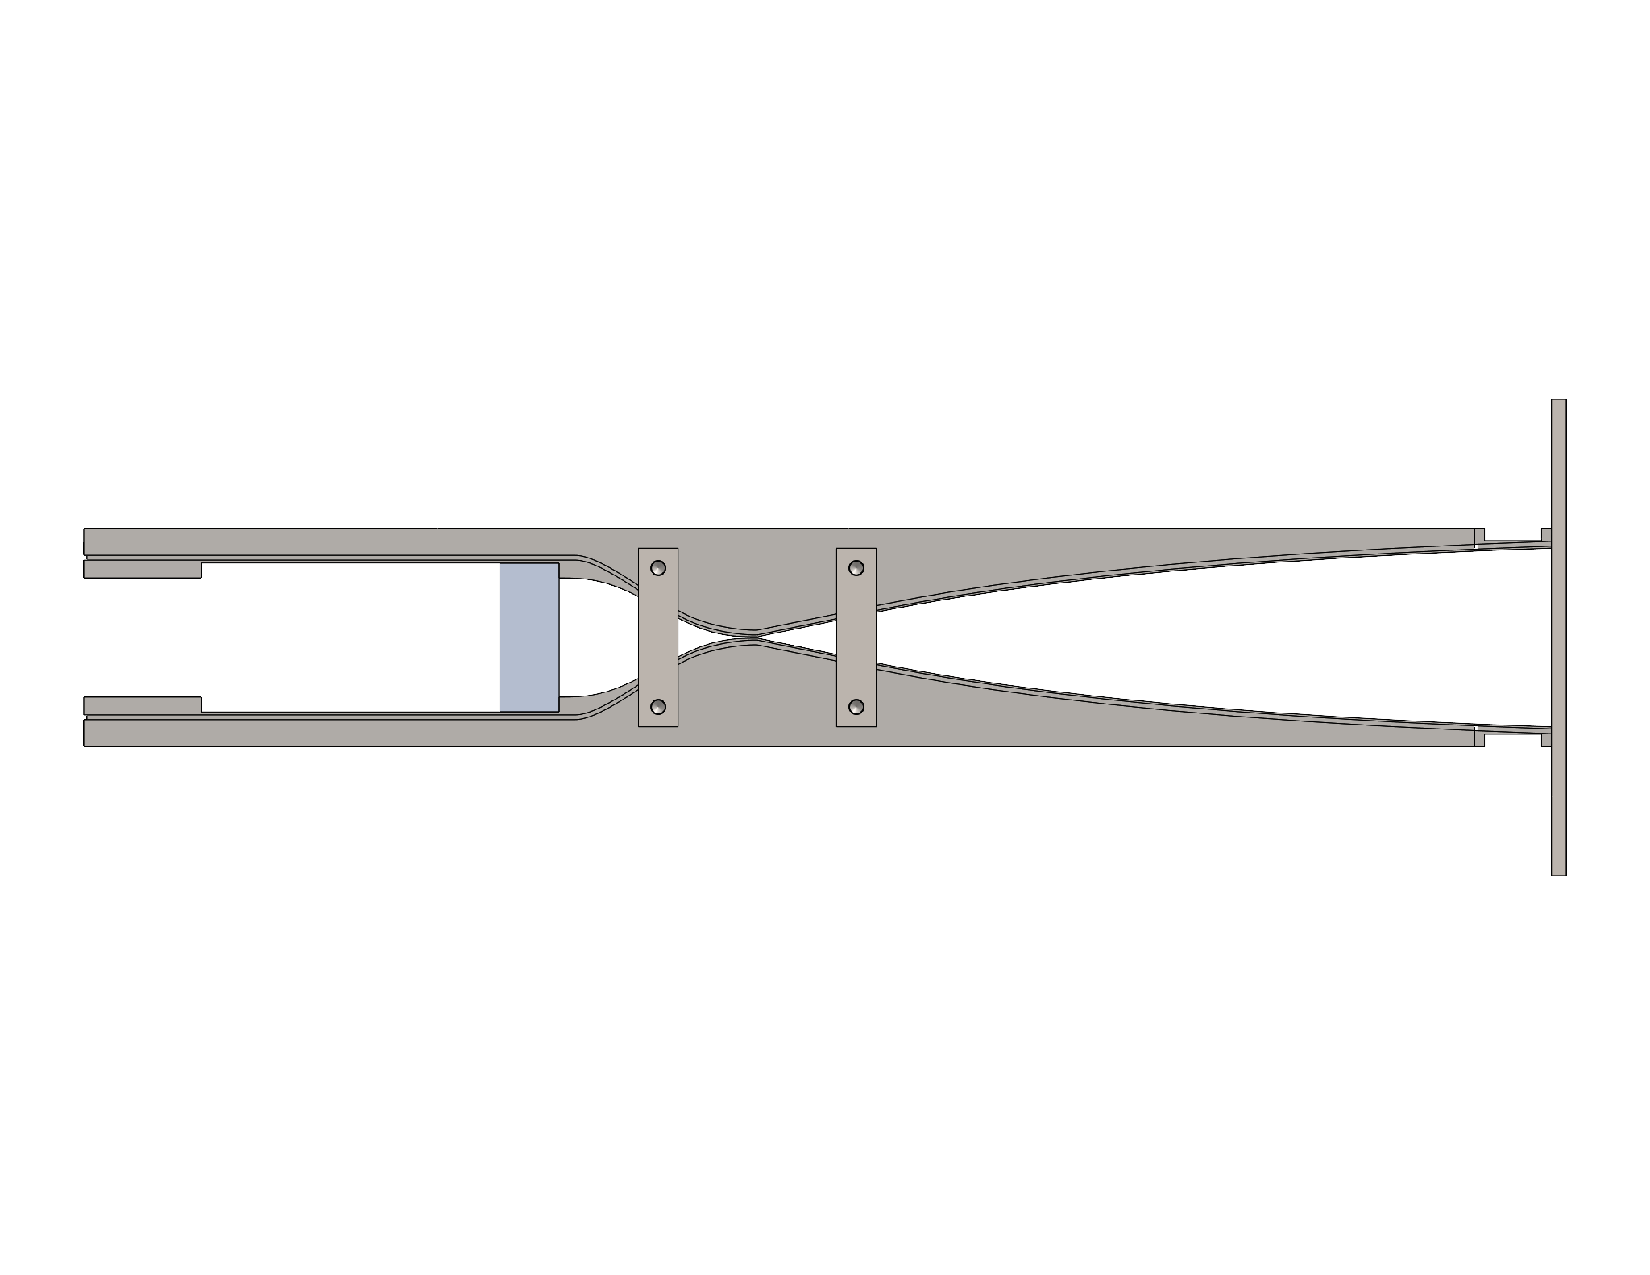
\includegraphics[trim={30 170 30 170},clip,width=5in]{polish-assembly.pdf}
    \caption{Nozzle assembly for shipping to polishing vendor.}
    \label{fig:polish-assembly}
\end{figure}

\section{Final Assembly, Installation, and Calibration}

The final assembly will occur at the NAHL once the nozzle and sidewalls are delivered from polishing. Once nozzles and actuators are assembled in the frame, ACE2.0 will be rolled into the lab to replace ACE. All hoses, wires, and instrumentation attached to the nozzle and settling chamber will be removed and ACE will be rolled out of the lab. ACE2.0 will roll in and reconnect all hoses, wires, and instrumentation.

\textcolor{red}{How to show assembly process? Discuss when we meet}

\subsubsection{Nozzle Alignment and Actuation Homing}

\textcolor{red}{How to properly align and level nozzle?}

Before the sidewalls are installed, the nozzles will be aligned and leveled and then actuated for homing the servo motors with the limit switches. At this point shims will be used to make fine adjustments to limit switch positions to ensure a minimum Mach number of \textcolor{red}{4.9?} and a maximum Mach number of \textcolor{red}{8.5?}.

\subsection{Shakedown and Calibration}

\textcolor{red}{Decide what the first runs and measurements should be to properly calibrate following relevant literature.}


%%%%%%%%%%%%%%%%%%%%%%%%%%%%%%%%%%%%%%%%%%%%%%%%%%%
%
%  Author: Jacob Vaughn
%  
%  Last Updated: 1/13/2024
%
%%%%%%%%%%%%%%%%%%%%%%%%%%%%%%%%%%%%%%%%%%%%%%%%%%%
%%%%%%%%%%%%%%%%%%%%%%%%%%%%%%%%%%%%%%%%%%%%%%%%%%%%%%%%%%%%%%%%%%%%%%
%%                       EXPERIMENTAL SETUP
%%%%%%%%%%%%%%%%%%%%%%%%%%%%%%%%%%%%%%%%%%%%%%%%%%%%%%%%%%%%%%%%%%%%%

\chapter{EXPERIMENTAL SETUP AND MEASUREMENTS}

\section{Nozzle Survey}

Stuff

\section{Mach Sweep Hysterisis}

Stuff

\section{Mach Sweep Constant Unit Reynolds Number}

Look into using control system (servo?) to control P0 to maintain constant Re' through Mach sweep. May need two valves in series and may need to anticipate mach change with P0 change ahead of time depending on response time.

% %%%%%%%%%%%%%%%%%%%%%%%%%%%%%%%%%%%%%%%%%%%%%%%%%%%
%
%  Author: Jacob Vaughn
%  
%  Last Updated: 1/13/2024
%
%%%%%%%%%%%%%%%%%%%%%%%%%%%%%%%%%%%%%%%%%%%%%%%%%%%
%%%%%%%%%%%%%%%%%%%%%%%%%%%%%%%%%%%%%%%%%%%%%%%%%%%%%%%%%%%%%%%%%%%%%%
%%                          RESULTS
%%%%%%%%%%%%%%%%%%%%%%%%%%%%%%%%%%%%%%%%%%%%%%%%%%%%%%%%%%%%%%%%%%%%%



\chapter{RESULTS AND DISCUSSION}

Stuff about experminet results

\begin{figure}[ht]
    \centering
    
\includegraphics[width=6in]{tamulogo}
    \caption{A caption about penguins}
\end{figure}

More stuff

\section{Maybe}

\section{Possibly}

%%%%%%%%%%%%%%%%%%%%%%%%%%%%%%%%%%%%%%%%%%%%%%%%%%%
%
%  Author: Jacob Vaughn
%  
%  Last Updated: 3/8/2024
%
%%%%%%%%%%%%%%%%%%%%%%%%%%%%%%%%%%%%%%%%%%%%%%%%%%%
%%%%%%%%%%%%%%%%%%%%%%%%%%%%%%%%%%%%%%%%%%%%%%%%%%%%%%%%%%%%%%%%%%%%%%
%%                         CONCLUSIONS
%%%%%%%%%%%%%%%%%%%%%%%%%%%%%%%%%%%%%%%%%%%%%%%%%%%%%%%%%%%%%%%%%%%%%%

\chapter{CONCLUSIONS}

\section{Concluding Remarks}

The path forward will follow the manufacturing schedule shown in Figure \ref{fig:schedule}. The pressure test will be performed as soon as the nozzles are finished machining, tentatively May 1, 2024. Depending on the results of the pressure test, the process could be anywhere from a single day to two weeks. Once complete though, the nozzles and sidewalls will be shipped to the polishing vendor, which should have a quick turn around of two weeks. Upon arrival to the NAHL, the full ACE2.0 nozzle will be finally assembled and installed. With proper planning prior to the final installation, the process should not take more than a week to begin shakedown and characterization.

In the meantime, the servo control program will be written between now and the pressure test. The Mach number feedback will be implemented, and the Reynolds number control capability will be explored and potentially implemented before the final install. Again, this will primarily depend on the test schedule for the M6QT and the amount of time needed to replace the manual valve with a controlled valve. 

The characterization and hysteresis experiments will be performed immediately following installation and initial calibration. The primary goal is to ensure complete function of ACE2.0 along with a demonstration of the capabilities and potential for future research. Additionally, the documentation for the nozzle operation will be written based on the best practices deduced throughout the experiments.

\section{Impact and Future Work}

Stuff

%%%%%%%%%%%%%%%
% End of body %
%%%%%%%%%%%%%%%

\nocite{aiaa-uncertainty-standard}
\nocite{anderson-fundamentals}
\nocite{anderson-compressible}


%%%%%%%%%%%%%%%%%%%%%%%%%%%%%%%%%%%%%%%%%%%%%%%%%%%%%%%%%%%%%
\let\oldbibitem\bibitem
\renewcommand{\bibitem}{\setlength{\itemsep}{0pt}\oldbibitem}
%%%%%%%%%%%%%%%%%%%%%%%%%%%%%%%%%%%%%%%%%%%%%%%%%%%%%%%%%%%%%%%
%The bibliography style declared is the IEEE format. If
%you require a different style, see the document
%bibstyles.pdf included in this package. This file,
%hosted by the University of Vienna, shows several
%bibliography styles and examples of in-text citation
%and a references page.
\bibliographystyle{ieeetr}

\phantomsection
\addcontentsline{toc}{chapter}{REFERENCES}

\renewcommand{\bibname}{{\normalsize\rm REFERENCES}}

\bibliography{prodata/myReference}

% Appendices main file
%%%%%%%%%%%%%%%%%%%%%%%%%%%%%%%%%%%%%%%%%%%%%%%%%%%
%
%  New template code for TAMU Theses and Dissertations starting Spring 2021.  
%
%
%  Author: Thesis Office
%  
%  Last Updated: 1/13/2021
%
%%%%%%%%%%%%%%%%%%%%%%%%%%%%%%%%%%%%%%%%%%%%%%%%%%%

\begin{appendices}
\titleformat{\chapter}{\centering\normalsize}{APPENDIX \thechapter}{0em}{\vskip .5\baselineskip\centering}
\renewcommand{\appendixname}{APPENDIX}

%%%%%%%%%%%%%%%%%%%%%%%%%%%%%%%%%%%%%%%%%%%%%%%%%%%
%
%  New template code for TAMU Theses and Dissertations starting Spring 2021.
%
%
%  Author: Thesis Office 
%	 
%  Last updated 1/13/2021
%
%%%%%%%%%%%%%%%%%%%%%%%%%%%%%%%%%%%%%%%%%%%%%%%%%%%

%%%%%%%%%%%%%%%%%%%%%%%%%%%%%%%%%%%%%%%%%%%%%%%%%%%%%%%%%%%%%%%%%%%%%%
%%                           APPENDIX A 
%%%%%%%%%%%%%%%%%%%%%%%%%%%%%%%%%%%%%%%%%%%%%%%%%%%%%%%%%%%%%%%%%%%%%

\phantomsection

\chapter{\uppercase{First Appendix}}

Text for the Appendix follows.

\begin{figure}[h]
\centering
\includegraphics[scale=.50]{Penguins.jpg}
\caption{TAMU figure}
\label{fig:tamu-fig5}
\end{figure}

%%%%%%%%%%%%%%%%%%%%%%%%%%%%%%%%%%%%%%%%%%%%%%%%%%%
%
%  New template code for TAMU Theses and Dissertations starting Spring 2021.
%
%
%  Author: Thesis Office 
%	 
%  Last updated 1/13/2021
%
%%%%%%%%%%%%%%%%%%%%%%%%%%%%%%%%%%%%%%%%%%%%%%%%%%%

%%%%%%%%%%%%%%%%%%%%%%%%%%%%%%%%%%%%%%%%%%%%%%%%%%%%%%%%%%%%%%%%%%%%%%
%%                           APPENDIX B
%%%%%%%%%%%%%%%%%%%%%%%%%%%%%%%%%%%%%%%%%%%%%%%%%%%%%%%%%%%%%%%%%%%%%

\chapter{\uppercase {This Title Is Much Longer Than The First and Extends All the Way to the Next Line}}

Text for the Appendix follows.

\begin{figure}[h]
\centering
\includegraphics[scale=.50]{figures/Penguins.jpg}
\caption{Another TAMU figure.}
\label{fig:tamu-fig6}
\end{figure}

\section{Appendix Section}

\section{Second Appendix Section}


\pagebreak{}

\end{appendices}

\end{document}
